\documentclass[14pt]{extbook} % Edit this line to change the documentclass.
% Add custom preamble content below.
% Example commands for using the Polyglossia package with French are
% included for reference.
% You may also have to edit config/lang.yml to sync up the HTML/EPUB/MOBI.
% \usepackage{polyglossia}
% \setdefaultlanguage{french}
% \DeclareTextCommandDefault{\nobreakspace}{\leavevmode\nobreak\ }

\usepackage{latex_styles/softcover}
\VerbatimFootnotes % Allows verbatim text in footnotes
\title{The Positioning Manual for Technical Firms}
\subtitle{v3 (BETA build 1)}
\author{Philip Morgan}
\date{}

\begin{document}

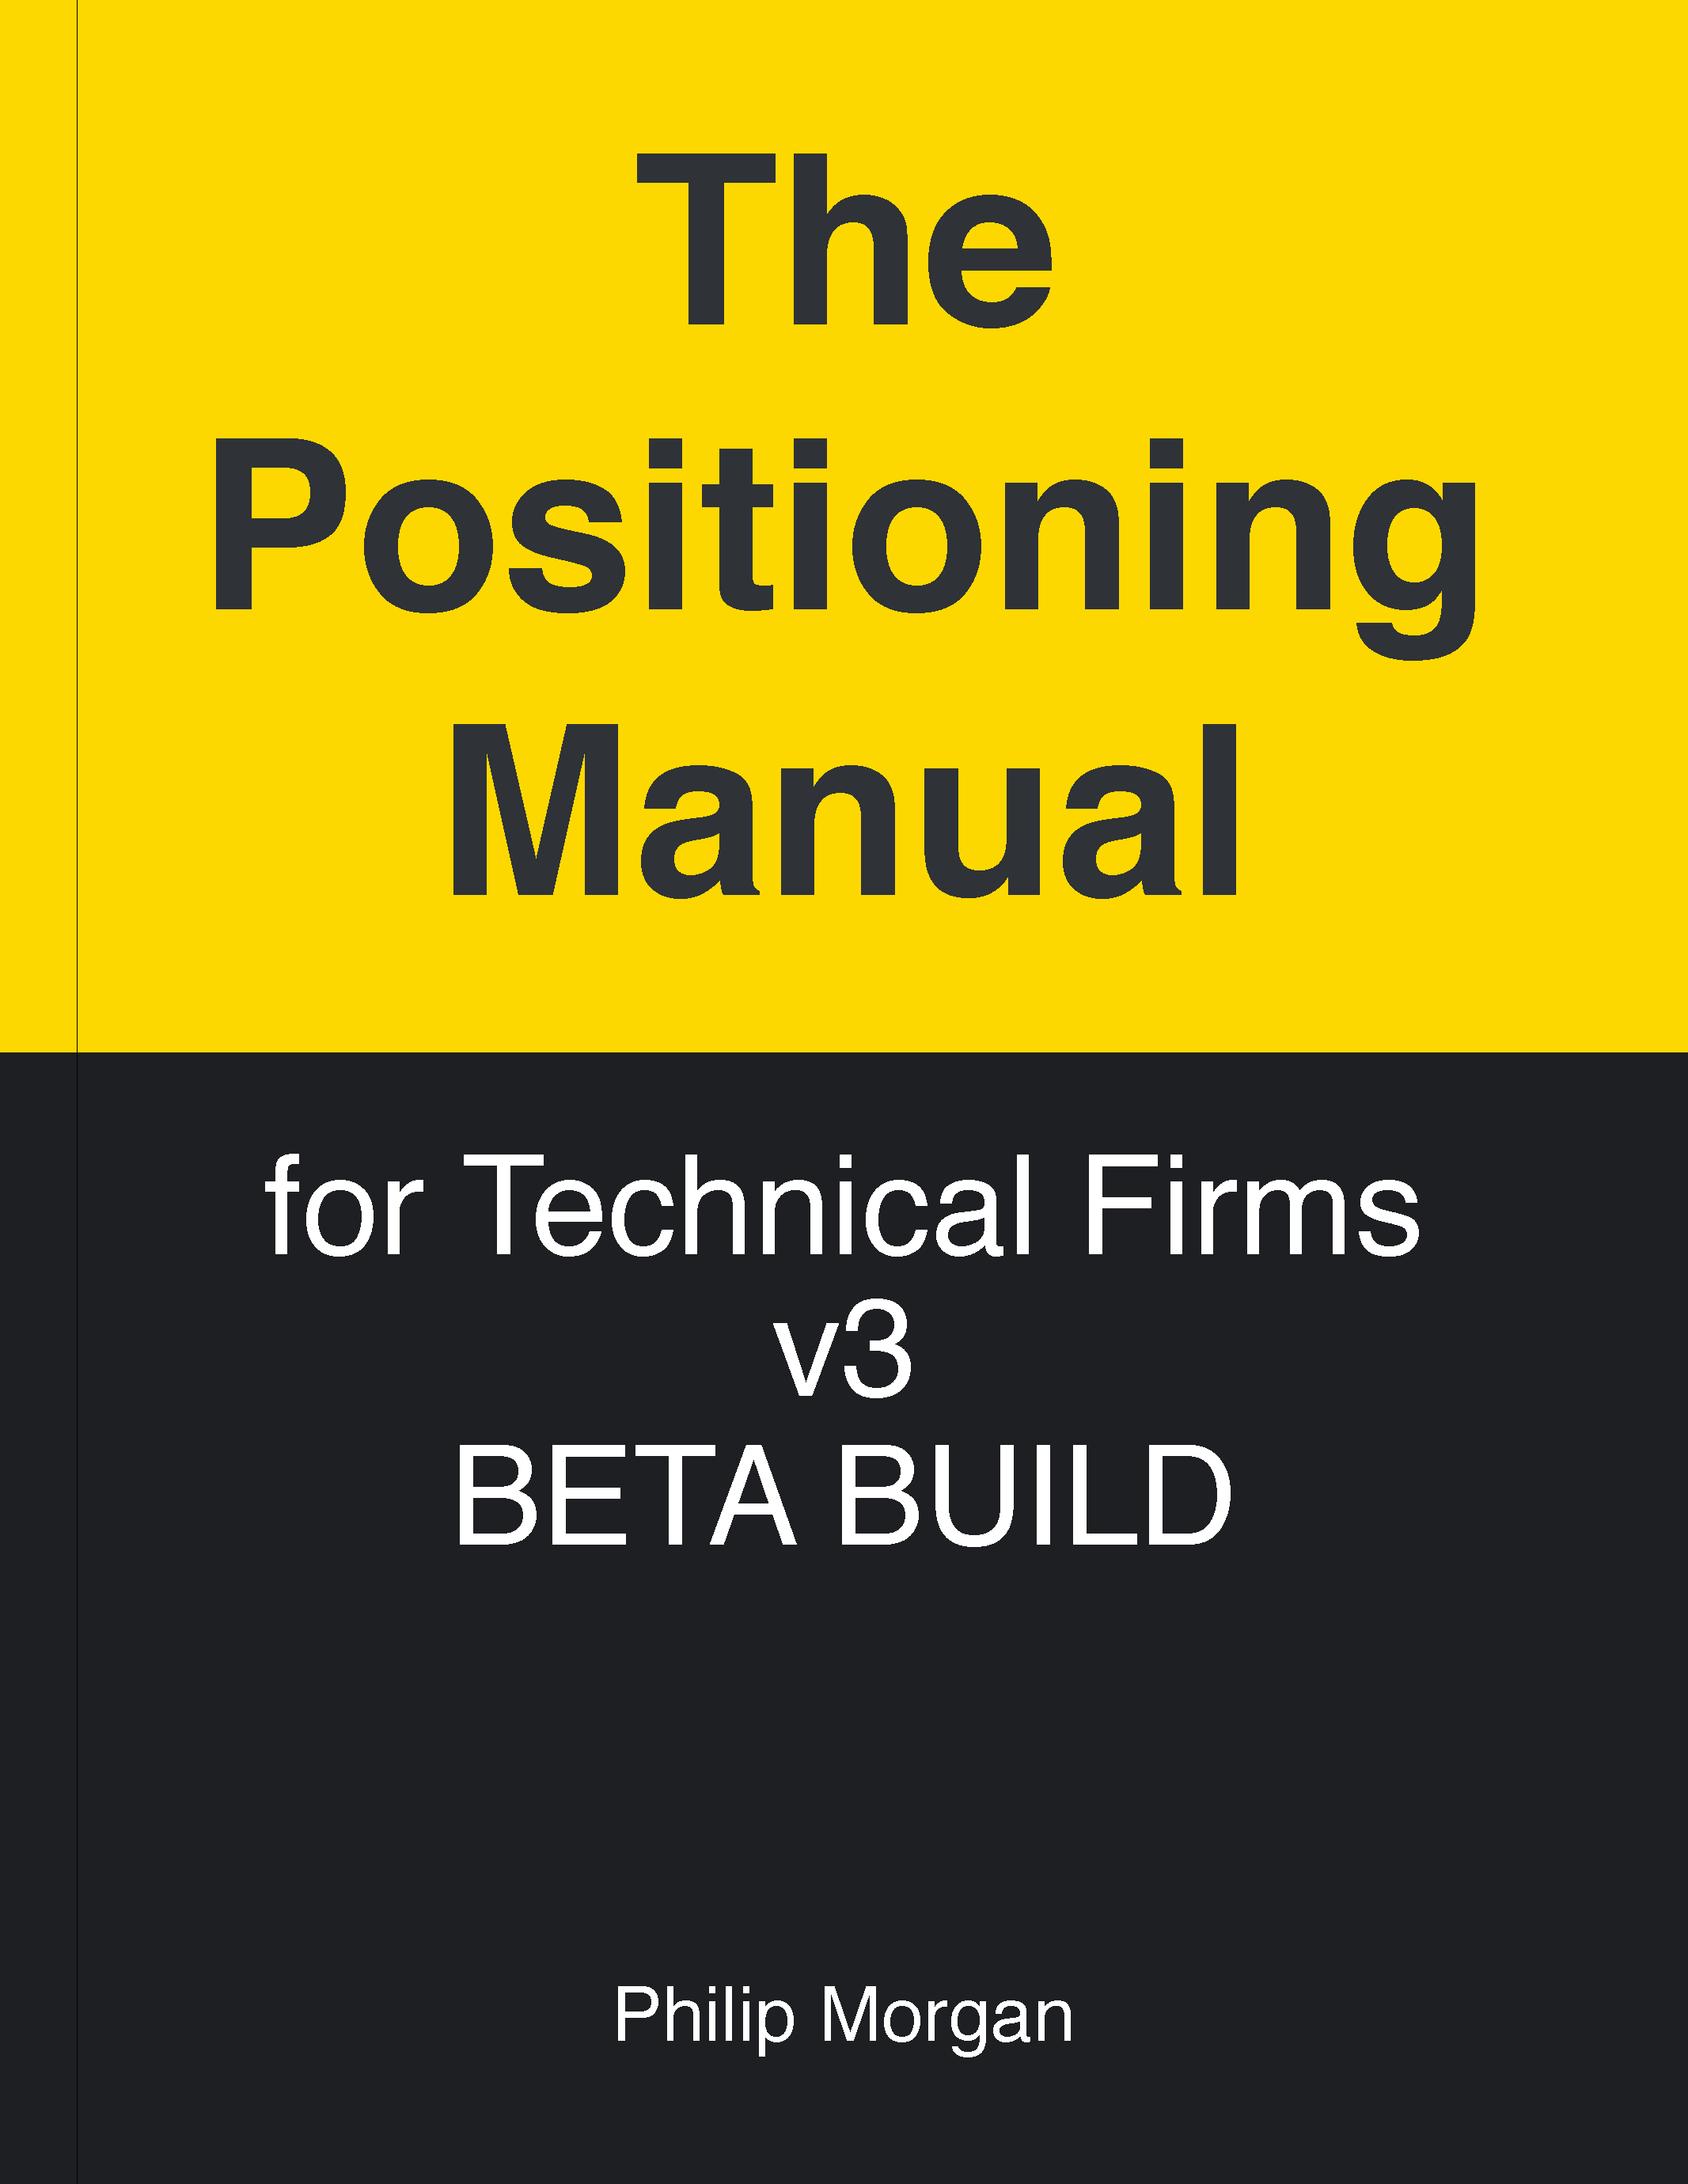
\includepdf{images/cover.pdf}
\frontmatter
\maketitle
I'm revising The Positioning Manual for Technical Firms. It's a big, messy revision.

While I'm revising the book, I'm working in public and making the draft fully available for free right here. The permalink for the book, if you wish to share it with anyone (please do!) is: \href{http://thepositioningmanual.com/v3}{http://thepositioningmanual.com/v3}.

After I finish revising the book, I'll continue to make it available for free in an inconvenient, somewhat un-beautiful form while charging money for more convenient or beautiful forms of the book.

So for now, you can read the entire book right here in HTML, or you can download an \href{../ebooks/TPM-v3.epub}{ePub}, \href{../ebooks/TPM-v3.mobi}{MOBI}, or \href{../ebooks/TPM-v3.pdf}{PDF} version of the book as well.

As the writing process continues, I'll update the book. If you want to get pinged when the book gets updated, \href{https://philipmorganconsulting.com/list}{join my email list}.
\tableofcontents
\chapter{Introduction}

I wrote the first version of TPM as an excited evangelist of an idea, and I wrote the second version as a diligent researcher seeking greater insight and fidelity. Now I approach this third version as a more seasoned practitioner, hoping my considerably deeper in-the-trenches experience translates to clearer thinking, better articulation of that thinking, and more practical, nuanced, and useful recommendations.

The updates to version 3 are numerous:

\begin{itemize}
\item Standardized terminology
\item More context around the business function of specialization
\item Way more context around the nuances of specialization
\item More grounded, practical recommendations based on your business maturity
\item More information on the relationship between specialization, your market position, and other common understandings of positioning
\item More information on the role of expertise in specialization, and recommendations on how you might aggressively cultivate valuable expertise
\item A different packaging and pricing model, with the same distribution model


\begin{itemize}
\item A tiered pricing approach is often very effective for maximizing info-product revenue. That's why I chose it for the second version of TPM. I needed the revenue, and it did just that. My business has matured since then, in large part thanks to TPM. My primary goal with this possibly final version of TPM is greater reach combined with access to buyers, but with the table tilted towards reach. That's why I'm pricing at \$19 for the electronic version and \$39 for print-on-demand. I believe it helps achieve the goal of greater reach.
\item I'm sticking with the self-published distribution model because I need the opportunity to connect with, build trust with, and further support book customers post-purchase. My business still needs this low-cost marketing approach to allow me to keep executing on the mission I'm here for. I felt good about the content in middle tier of the old version of TPM, which included a bunch of helpful guidance for implementation, but with this version I'm taking some of that content and pushing it down into what would have been the base tier of the old version (and is now the only tier of the new version), and taking other parts of that old middle tier content and replacing it with a group of pretty affordably priced online courses. Those courses are an upsell to the book, offered online and within the book itself, and they're a nice way of letting customers self-select the right level of implementation support. Those that are execution machines can take the ideas contained in the \$19 book and run with them on their own. They won't be manipulated by a pricing scheme into buying the old \$99 middle tier of TPM ``just in case'' they need that extra info. They will have gotten an amazing ROI at \$19 or \$39. Those that need more detailed guidance on execution make that decision after making the minimal investment in the \$19 book and they can then move on to buy one or more \$150 online courses if they see the need. They'll be motivated buyers because they've proven to themselves the book was good but not enough detailed guidance. They'll get great ROI from these courses, and I hope they feel that they bought them based on an actual need they've demonstrated to themselves rather than the psychological pressure of a tiered pricing scheme.
\item I'm not at the point in my businesses maturity (yet) where a full mass-market \emph{distribution model} (partnering with a publisher or self-publishing on Amazon's Kindle store) makes sense because that would deprive me of low-cost access to my book customers via email, but a more mass-market \emph{pricing model} does make sense, because it trades revenue for reach, and I'm ready to make that tradeoff.
\item I keep wanting to do an audio version, and I keep putting that off because of my perception of how difficult it would be to get it \emph{right}. But maybe one of these days\ldots{}
\end{itemize}
\end{itemize}

\section{How to Use This Book}

Just read it straight through. Each chapter is better than the one before it! Chapter 12 is a sort of climax, but making the best use of that chapter depends 100\% on understanding everything that comes before it in this book.
\mainmatter
\chapter{Why Position Your Company?}

TODO: revision notes

\begin{itemize}
\item Perhaps reference DCB’s hourly rate research. Mention profitability.
\item Pre-req to value pricing
\item Better clients
\item Better business
\item happier you
\end{itemize}

This manual is over 23,000 words on how to develop a desirable market position for your business. But the question of \emph{why} to do this is easily answered in just 4 words:

\textbf{Better clients, higher fees}

If you're used to thinking in terms of hourly, daily, or weekly rates instead of per-project fees, that's fine--the benefits of a narrow market position still apply to you. Better clients, higher \emph{rates}.

\section{But Wait, There's More!}

Those are just the headline benefits of a narrow market position. Even more benefits appear when you really look closely. To thoroughly understand the benefits, let's take a step back and assess the situation you're probably in if your business does not focus on a narrow market position.

\subsection{1) \textbf{You started working for yourself with little preparation}.}

You didn't study the world of business for months or years before making the leap to self-employment. Instead, the move to self-employment was more\ldots{} improvised. An unexpected layoff, a shitty boss you were fed up with working for, or an unexpected offer of contract work might have been what caused you to make the leap to self employment.

This was \emph{exactly} how I became self-employed. I had a great boss but got laid off in 2008 (along with everybody else at my employer), coasted on unemployment for a few months, and then said, ``Screw it, I can be self-employed!''. I then proceeded to spend 5 years beating my head against the brick wall of being an undifferentiated generalist while constantly facing the prospect of financial ruin and a shameful retreat to the ``safety'' of a FTE job.

\subsection{2) \textbf{Business development is either an afterthought, a struggle, or both}.}

If you had to sum up your business development approach in one word, it would be \textbf{luck}, or maybe \textbf{hustle}. Maybe you hope for a lucky break while refilling your drink at those depressing networking events where 75\% of the crowd is unemployed freelancers, and the other 25\% is big agencies scouting for cheap talent to put into the next project grinder.

Maybe you depend a little too much on referrals from past clients. And maybe your outreach to prospects is based on a generalist value proposition and a lot of hustle, as in cold email blasts saying something like\ldots{}

\begin{quote}
We can handle all of your development/design/marketing needs. We're a \emph{full service} agency!
\end{quote}

Finally, you are \emph{almost never} sought out because your services solve a very specific, expensive problem for a client. Instead, you win jobs because you are affordable, ``great to work with”, or seem more ``together'' than the alternatives.

\subsection{3) \textbf{You operate from a position of weakness in rate/fee negotiations}.}

Your rate or fee is dependent on how badly you need or want whatever work is on the negotiating table, and you offer discounts (even when they're not asked for) based on your eagerness to win the work or the level of anxiety you are feeling around your pipeline. You offer payment terms that are extremely generous (more than 7 days net) to every client, after the contract is signed you are shuffled off to the client's finance/accounting department where you are treated like a low-level vendor rather than a valued business partner, and when payment is late you automatically assume the position of a supplicant and make tense, carefully worded requests for payments to low-level bureaucrats within your client's finance/accounting department.

\subsection{4) \textbf{Your business feels like it is treading water}.}

Perhaps you are growing very slowly, or perhaps your growth has already plateaued and is limited to 10\% or 20\% a year ``cost of living'' rate increases that are met with grumbling acquiescence from clients. Your business growth strategy is  ``more of the same'' or\ldots{} hope, and you take little time to focus on finding new ways of creating value for clients.

\subsection{5) \textbf{You almost never say no to work}.}

Every project that does come your way is met with an enthusiastic ``Sure, we can do that!'' and a mad scramble to put together a creative, persuasive proposal as quickly as possible. After you pitch or email in your proposal, you find yourself on pins and needles while you wait to hear the results.

You really have no idea whether you will win the work, and you check in with your prospective client periodically to diplomatically ask how the decision process is going.

If any of this rings true for you, I want to reiterate that I was in this \emph{exact situation} for 5 years. Every painful thing I've listed above is something I've experienced firsthand, many times over. I've been there, it sucks, and there is a way out.

If you're \emph{not} in this situation because you've already focused your business on a great market position or have found some other way to charge premium rates and develop a strong pipeline of interesting, challenging work, \emph{go buy yourself an ice cream right now!} You've earned it, and you can skip reading the rest of this manual.

However, if any of the above rings true for you, then let me tell you how becoming a leader in a narrow market position will improve your condition.

I suppose this is the right place to say you \emph{could} position your business as an undifferentiated generalist. This would technically still be a form of positioning. However, it would solve no business problems at all for you, so in this manual I'm only going to talk about narrowing your focus in a way that positions you as a leader. In fact, any time I refer to positioning in this manual, that's what I mean: becoming a leader in a narrow market position. There really is no other way to position a professional services firm for maximum success.

\section{The Benefits of a Narrow Market Position}

In addition to giving you access to better clients and higher fees, becoming a leader in a narrow market position will make each one of the items I called out above \emph{much, much better}! Let's look at each one in turn:

\subsection{1) \textbf{You started working for yourself with little preparation}.}

Positioning is not a time machine that can go back and fix your past unpreparedness. But, when you position your business correctly, you finally address the root cause of \emph{so, so many} business problems. You \textbf{finally decide} exactly who you serve, what you do for them, and how you are different from others doing similar work. Making this choice is a pre-requisite for solving other business problems like fee-setting, billing, and client relationship problems. Making this choice is the \textbf{foundation} for building a robust professional services business.

We can learn a lot from product businesses. So much of the strength of a good product business comes from the product itself. How well does it address a real need, how well-designed and marketed is it, how efficiently can it be produced, distributed, and maintained?

Without a well-designed product that meets a real need or desire in the market, you don't have a product business--you have a mess. That's patently obvious, yet in the world of professional services, many firms operate with no equivalent to a product. Their services are so ill-defined and broadly scoped that potential buyers have no idea what need or desire those services match up with.

Focus is just as important to a professional services firm as it is to a product business.

\subsection{2) \textbf{Business development is either an afterthought, a struggle, or both}.}

The linchpin of a business development strategy is positioning. If you are, for example, a ``Rails shop'' or a ``front-end developer'' or a ``CTO for hire'', you are in direct competition with every other human being who is using the same label for their business (fn1). When your target is that broad, that's a \emph{lot} of competition, as I'm sure you know from direct experience. Furthermore, you have no ``unfair advantage'' over that competition, and you depend fundamentally on luck or an extraordinarily helpful professional network to bring you in contact with clients who are a great fit for you.

Yet, if you focus on a narrow market position, the game changes \emph{completely}. If, instead of a ``Rails shop'' you are a company that ``builds modern reporting systems on top of legacy systems data to reduce damaged freight insurance claims for large privately held freight companies by up to 40\%'' (fn2), your approach to business development becomes dramatically more efficient \emph{and} effective. Here’s why:

\begin{itemize}
\item You can very quickly have a list of prospective clients. Not just a list of \emph{types} of companies that could be your clients but a list of \emph{specific} companies with names of \emph{specific} people you can market to, meet with, and get signed checks from. You intersect a list of large freight companies with a list of users of legacy systems and \emph{boom}, you have a prospect list that--if you have chosen a niche of the right size—will keep your company fed, growing, and winning almost every project you want for a long time. Getting this information is not complicated, and once you have it, you have a huge part of your game plan for business development locked in.
\item Your value proposition to that list of prospects stands out in a crowd like a red Ferrari in a parking lot full of gray station wagons. When those prospects become aware that it's possible to save millions or tens of millions of dollars a year in insurance claims \emph{and} that there's a company with a track record of reliably creating that \emph{exact outcome}, your business development becomes like ``selling water to a thirsty person in a desert'' rather than ``selling ice to an Eskimo''.
\end{itemize}

\subsection{3) \textbf{You operate from a position of weakness in rate/fee negotiations}.}

To return to the previous example in \#2 above, if you have chosen a market position that sets you up to solve a very specific, expensive problem for clients like the software solution that saves millions in damaged freight insurance claims, then the power dynamic shifts in your favor. Remember, ``expensive problems'' may be ones where solving the problem produces an impressive return on investment (ROI), or a significant cost savings.(fn3)

A solver of expensive problems becomes a partner rather than a vendor, and partners are entitled to an equitable share of the results of the partnership. Partners get to speak up for themselves when they don't like the terms of the agreement, while vendors have to ``go along to get along'' or risk being replaced. If the options for replacing you are very limited, you naturally have much more power in the relationship.

\subsection{4) \textbf{Your business feels like it is treading water}.}

If you are a generalist doing some kind of technical work like programming or web development, you are likely able to charge \$75 to \$150 USD an hour. If you are billing in that range, how much professional development (within business hours) can you allocate the time and funds for? How much time can you spend developing new services, products, or entire lines of business?

Your ability to grow your business in innovative new ways is limited if you are spending 75\% or more of your time doing billable work. Operating as a focused specialist gives you access to dramatically higher rates (often \$200/hr and above) or the ability to apply value-based fees to projects because you are solving an expensive problem. This means that you can spend a greater portion of your time moving your business out of water-treading mode.

\subsection{5) \textbf{You almost never say no to work}.}

This is one of the benefits of being a focused specialist that you just have to experience to fully appreciate. I really can't tell you how much emotional energy I burned up because, as a generalist, I was in a financial position where I really needed to say ``yes'' to every project that came my way.

Later on in the projects that became nightmares, I would ask myself ``honestly Philip, did you see this coming before the contract was signed? Was there some sign that was right there in front of your face?'' The answer was \emph{always} yes. The nightmare client had \emph{always} given some sign of what was to come: balking at my rates, communicating with me only at their convenience, or some other red flag that later made the project very painful. Or in other cases, I had taken on a project that was at or beyond the limits of my expertise, making the project painful for a different set of reasons.

A focused specialist can say no to a good portion of the clients that come their way if necessary. Quality of work life goes up dramatically as a result of the ability to throughly vet prospects based on what really will produce a good fit for both client and consultant.

\section{Conclusion}

In conclusion, remember that finding a narrow market position is the most efficient way to deal with the common issues that lead to a “feast/famine” cycle in your business.

\section{Footnotes}

Of course, this may be a smaller pool of competitors too in cases where a client wants to work only with a local company, etc. But more and more, especially in technology services, clients are sourcing from a global pool of talent.

This is a hyper-specific example, mostly to make a point. You do not have to be this specific in your messaging, but you must be quite a bit more specific than you probably have been thus far.

Incidentally, properly positioning your business produces both a strong ROI and a cost savings to you as well. The ROI comes from your future ability to attract better clients and charge higher fees, and the savings from having fewer clients that are a poor match for your business.
\chapter{Who This Manual is For}

I sincerely hope this manual is extremely useful to you as you attempt to solve one of the most common problems in individually owned technical services firms: the lack of proper positioning.  If at any point in working your way through this manual you run across problems, I encourage you to contact me directly. I'm Philip Morgan, and I help custom software development shops get more leads without hiring a sales person. I use positioning, education-based content marketing, and marketing automation to make that happen. You can reach me via email at \href{mailto:philip@philipmorganconsulting.com}{philip@philipmorganconsulting.com}.

\section{Who This Manual is For}

This manual will be most helpful to a narrow range of people:

\begin{itemize}
\item Owners of technical services firms like programming consultancies, web or digital agencies, and SaaS companies.
\item Independent consultants or freelancers of many stripes, though all my examples in this manual are specific to the technical rather than the creative end of the professional services spectrum.
\item People who are considering making the leap to solo self-employment but haven't done it yet.
\item Self-employed people who need to be making more money within 12 months, but can invest 6 months of effort to lay the foundation.
\end{itemize}

This manual will \emph{not} be immediately helpful to you if you have very limited work experience or ``the wolf is at the door'' in terms of your finances. Developing a desirable market position requires discipline in client selection and negotiation that will be very difficult to muster if you have little savings, credit, or leeway in terms of saying no to work in the short term. Making a good positioning choice requires a certain amount of self-awareness about your strengths and preferences, and you just can't discover that stuff without a year or two of full-time client work under your belt.

Finally, this manual is meant to be concise. How many 80,000-word business books have you read that should have been 20,000 words? So many business books are one meaningful but straightforward insight padded out with redundant content to make a publisher happy. This one is not.

Even with a few interruptions you should be able to read this book cover to cover in 2 hours or less. I’m confident you’ll get a \emph{world class} ROI on that modest time investment.
\chapter{It's Gonna Hurt}

\section{Why is Positioning so Difficult?}

I wouldn't be writing this manual if properly positioning a privately owned technical services firm was easy. And you wouldn't be reading either if it was easy.

So why is it not easy?

\subsection{It Brings Up The Fear}

Know that \emph{you will face some gnarly fears} as you move through the work of narrowing your business focus so that you can provide more value to your clients. Moving from operating as a generalist, ``A to Z'', or ``full service'' firm to operating as a focused specialist will almost certainly cause you to fear that:

\begin{itemize}
\item You have chosen the wrong thing to focus on
\item You are not worthy of commanding premium rates for your work
\item You are cutting off access to desirable, profitable work
\item You will quickly become bored with your choice
\end{itemize}

Collectively, I call these fears \emph{The Fear}.

\subsection{It Challenges Your Sense of Identity}

Properly positioning your professional services business is also difficult because it is \emph{so personal}. A lot of us start our self-employment under a personal brand. We don't really think of ourselves the way that a manufacturer of backpacks or wallets or speed controllers for electric motors would think of their business. They would almost certainly have a non-personal business identity from day 1.

When we in the professional services business try to develop a narrow market position, it's so wrapped up in our \emph{identity} of who we are, even if we have a non-personal business name. We are creative people, and we love the thrill of exploration and new learning curves. Even more, we often take real pride in how our personality attributes are woven into our businesses.

It comes with the territory of being creative that we \emph{don't} like to think of ourselves as narrow specialists. In fact, we jump to unfairly characterizing narrow specialists as ``one-dimensional'', ``wonks'', and even ``boring'', while we neglect the incredible potential for exploring the intricate \emph{depth} of a specialty.

\subsection{It's Mysterious}

Using positioning to your advantage is also \emph{mysterious}. For beginner business owners, it's not 100\% apparent that dramatically narrowing your focus is one of the keys to opening up access to higher fees and better clients\footnote{Proper pricing and effective marketing are the other two keys.}. We think that the path to those forms of financial and career success lies in expanding our skill set to the bleeding edge, networking, simply demanding higher rates or fees, a fancy new web site, or some other less difficult way.

\section{Positioning is Vital}

If you want to gain access to higher fees and better clients, there are many things you can try. You can do things like the aforementioned expanded skill set, networking, demanding higher rates or fees, or a fancy new web site. There are four other approaches that largely bypass the need to narrow down your focus:

\begin{enumerate}
\item \textbf{Luck}: I lucked into \$150k worth of work when I started working for myself. Luck giveth… and later luck took that work away with no prior notice, so beware relying too much on luck.
\item \textbf{Connections}: Knowing the right people can be a temporary substitute for becoming mature and disciplined in your business development.
\item \textbf{Leverage an offshore team}: Taking advantage of the rate differential between what developed country clients are willing to pay and rates charged by talent from low cost of living areas can be a solid way to run a business without narrowing down your focus. You may miss out on the ability to be selective about your clients, but you’ll have a reasonable business anyway.
\item \textbf{Ride a platform that is crossing the chasm to mainstream status}: From about 2008 to the time of this writing in mid-2016 (and perhaps slightly beyond), the only business development a good iOS developer needed to do was to keep their LinkedIn profile up to date. A platform exploding in popularity can be a temporary substitute for a narrow market position.
\end{enumerate}

If any of those methods work for you:

\begin{enumerate}
\item \textbf{Congratulations}--seriously--congrats on the quick win!
\item \emph{Be careful}, because you have likely come across a non-repeatable one-off win that will not result in sustained growth for your business.
\end{enumerate}

There is only one repeatable path to premium rates and better clients that is under your control, and that path involves narrowing your focus in order to increase the value you deliver to clients. This path sets you up for sustainable growth, and solves a myriad of problems in your business.

\section{You Will Face The Fear}

If you specialize your marketing, you will for sure face The Fear. Because of The Fear, I find that many people tend to retreat into generalizations and excuses to not position their business as a specialist.

I can identify. I resisted specializing for the first 5 years I worked for myself. At first, it was because being a generalist seemed more interesting and exciting, and I didn't understand the benefits of specialization. Then, it was because of The Fear. Eventually, I transitioned away from being a generalist writer for anybody with a pulse and a checkbook to my current specialized focus. But I lived on the brink of financial ruin for those 5 stressful years before specializing. Anything that made an already-precarious situation seem more risky was not a welcome change. So I get it\ldots{} narrowing your focus is a challenging process!

Here were my fears about positioning myself as a specialist. I'd bet money they are the same ones you face when you consider specializing:

\begin{quotation}
What if I pick the wrong niche?

What if I am unknowingly committing career suicide?

What if I can't deliver on my claims of expertise?

What if I pick a \textbf{really boring} niche and before I know it I'm crying myself to sleep every night on \$900 silk sheets while my soul slowly dies?
\end{quotation}

The good news is threefold:

\begin{enumerate}
\item Almost every person who has positioned themselves as a specialist has good things to say about it.
\item The Fear is pretty common to everyone who makes this transition. By knowing what to expect, the entire process will be a business development power play on your part rather than an exercise in battling your own demons.
\item There are ways to reduce the risk of what feels like a \emph{very risky} transition. You do not have to bet the farm on a new, untested positioning.
\end{enumerate}

\section{The Fear}

As you develop a new market position, be prepared to experience these four common fears.

\subsection{Loss Aversion}

You will at some point feel like you are excluding desirable clients by narrowing your marketing and by saying no to clients that you could potentially help but fall outside your defined focus.

The truth is that you \emph{are} doing this, but you are \emph{also} opening up access to a more \emph{profitable, desirable, deeper niche market} that has greater earning potential for you. You cannot gain access to that niche market without becoming focused and demonstrating your expertise through your marketing.

\subsection{Imposter Syndrome}

Unless you are an unusually self-confident person, you will question your expertise and your worthiness to charge \$200/hr plus\footnote{That's just an example of a rate that's well beyond generalist territory. Of course, your mileage may vary.}. This goes away after a while, but I believe this particular fear does cause some people to shrink back from the path of specialization, because deep down they know that they must believe in their own value, and they really don't at first.

The good news is that with focus comes confidence. If you are a generalist, you are \emph{always} dealing with learning curve and unexpected issues. When you specialize, you quickly learn how to deal with these common issues and your confidence increases \emph{very quickly} as a result.

This confidence will give you the strength you need to tackle bigger challenges within your area of focus. Tackling those bigger challenges will help you believe in your own value. This self-reinforcing feedback loop will quickly put an end to your imposter syndrome.

\subsection{Boredom}

It's common to fear that if you specialize, you will become bored with your work very quickly because you are narrowing the scope of what you do. In other words, you are solving a narrower range of problems for clients. You may fear that ``doing the same thing over and over again'' will get boring.

The fear of boredom is a false fear, rooted in an unrealistic picture of what it is really like to specialize. To outsiders, the world of specialization is perceived like that gray, drab world depicted in Apple's famous \href{http://bit.ly/1xEXr8B}{``1984'' TV commercial}. Those who inhabit it are perceived as robotic geeks who lack the interpersonal skills needed to communicate with others, or who are so consumed with their own enthusiasm for a narrow topic that they simple can't relate to others.

To get a more realistic picture of specialization ask yourself: ``who gives the most interesting \href{http://ted.com}{TED talks}? Generalists or specialists?'' In fact, who gives \emph{any kind of TED talk}?

\textbf{Specialists get invited to speak at TED}.

Specialists get to solve interesting problems \emph{all the time}. Solving interesting problems is not doing the same thing over and over again, it's drawing close and going deep into a subject. Specialization may from time to time involve tedious or unpleasant work to be sure, but who can better afford to hire help with those tasks? A \$90/hr generalist, or a \$350/hr specialist?

\subsection{Fear of Shrinking Brain Syndrome}

Finally, I have to mention that for almost any person working in the technical end of professional services (software development, IT, etc.), much of our identity is wrapped up in \emph{how much we know}. I'm no different--it's a point of pride for me to understand a wide range of subjects at some depth. I want to be perceived as being intelligent and current on a range of issues.

I think we technical folks fear specialization in part because we won't want to narrow down our knowledge domain, and we don't want to give up our identity as people who can speak intelligently to and actually solve a wide range of problems. Ultimately, we don't want to have to say, ``I can't help you with that.''

Again, this particular fear is a symptom of misunderstanding the pleasures of going deep with a specific subject. Furthermore, your business positioning may have little to do with the subjects you explore in your down time. And again I'll ask, who can afford more down time to explore matters of personal interest--a \$90/hr generalist or a \$350/hr specialist? Yes, you may have to adjust your expectations around getting paid to learn on the job--which is one of the ways the \$90/hr generalist gets to tinker with so many interesting toys ``on the clock''--but I trust you can see the benefits of making that shift.

\subsection{Picking the Wrong Niche}

The final fear is probably the most insidious, because it is psychologically complex. It involves both \href{https://en.wikipedia.org/wiki/Loss_aversion}{loss aversion} and \href{http://en.wikipedia.org/wiki/Analysis_paralysis}{analysis paralysis}, and the two seem to play off each other.

When you move from ``A to Z software development'' to a specialized subset of that work for a well-defined market vertical, it \emph{feels} like you are facing a \emph{tremendous loss} of potential work. You wonder if your chosen niche is large enough to support your continued growth. And then when you try to pick one of the \emph{many} things you could do to create value for clients, you get overwhelmed at all the choices!

If you are used to a ``take all comers'' approach to business development, making a choice and putting a stake in the ground feels incredibly risky. You are used to perceiving yourself as ``following the money'', and you can fool yourself into thinking that it's ``smart'' to be ``flexible'' and ``accommodating'' of the variety of clients that come your way. This mindset will tell you that choosing a single type of client to work with is like rolling the dice or playing Russian Roulette: very, very risky.

While I can't completely de-risk this choice for you, I will provide as many tools as I can in this manual to help you make a prudent choice about which market position to pursue.

\section{Let's Do This Together}

The rest of this book is all about helping you move through these fears and make the best positioning choice you can. There is a reason why Blair Enns calls positioning ``\href{http://www.winwithoutpitching.com/read-it-online/the-purpose-of-positioning/}{the Difficult Business Decision}''! It takes courage and commitment to push through the fear.

\section{Conclusion}

In conclusion, remember that the biggest obstacle to finding a desirable market position is not a crowded market place or strong competition. It’s the fears that naturally arise during the process.
\chapter{Positioning vs. Specialization}

When I ask you to think of the \emph{best} cloud platform as a service, what company or platform do you think of?

No matter whether you thought of AWS, GCP, Digital Ocean, or one of dozens of other cloud providers, you are responding to that product or company's \emph{reputation}. That reputation may be private to you, or it may be shared among a group of people. Here's what I mean.

There's a product called Zencastr that records podcasts interviews using a browser-based, double-ended approach. Zencastr has a generally positive reputation among the group of podcasters that I am friends with, but I have a very negative view of Zencastr. The product's ``private'' reputation with me as an individual is in tatters because the product failed me the two times I tried it. That's a 100\% failure rate! Others have had different experiences with a more favorable success rate.

It's no surprise that I personally dislike Zencastr and avoid using it while others who are demographically similar to me like it and prefer to use it. The product's reputation as it exists inside my mind is not good, while its reputation as it exists inside the mind of my peer group is very different, and much more positive. Same product, multiple reputations.

\textbf{A reputation that is similar across a group of people is also known as a \emph{market position}.}

Shall we play a game?

Either physically or mentally, make a dot on the diagram below. Where you place the dot should accurately describe your perception of two product lines. One dot for Apple's products, and another dot for Facebook's products.

\{TODO:Blank 2x2 matrix with cost on one axis and security on the other\}

Show and tell time. How much does your diagram look like mine?

\{TODO:My filled-in 2x2\}

Just notice how similar or different your placement of Apple and Facebook's dots are to mine. It's not that mine are ``right'' and yours are or aren't ``right''. That's not the point here at all, because there is no right or wrong placement of dots. Instead, the dots tell us something about Apple and Facebook's reputations \emph{as they exist inside my mind and your mind}.

Let's revisit the Zencaster example. Here's a similar 2x2 matrix showing Zencastr's reputation as it exists in my mind compares to how it exists in the minds of my podcaster friends:

\{TODO: 2x2 with value of features on one axis and reliability on the other, with a cluster of dots from my peers in the high value, reasonably reliable quadrant and my lone dot on the high value, low reliability quadrant\}

\textbf{Generally, the more consistency there is in the placement--or \emph{positioning}--of Apple, Facebook, Zencastr, or any business on a diagram like this, the more widely shared and homogenous that companies reputation--or market position--is.}

There's a seeming contradiction in this idea of a market position. If we could survey every living human, we would probably find very few businesses with a highly homogenous market position. If we could ask every living human to place Apple and Facebook on our 2x2 matrix, we'd find lots of variances because people have a wide range of preferences and worldview filters. If different people place--or \emph{position}--the same product or company in different positions on this matrix, how can any company have a clearly defined market position? Said differently, how can any company know how its products or services are perceived by the market?

In practice, this is not actually a problem, and it's especially un-problematic for \emph{you} because most companies and definitely yours will \emph{never} need to be perceived in precisely the same way by every human on the planet. Most small services businesses can get away with the right group of 1,000 to 10,000 people perceiving them the ``right'' way. Helping that many people perceive you the way you want to be perceived is still no small feat, but it's infinitely more achievable than trying to help every human on the planet perceive you the way you want to be perceived.

\textbf{A market position--again, your \emph{reputation}--is how you are perceived by the group of people who need to know about you for your business to thrive.}

This ``group of people who need to know about you for your business to thrive'' thing is important. We marketers have a shorthand for this: your \emph{target market}.

Lots of us who start out as freelancers and then graduate to consultants or entrepreneurs or agency owners start out with an accidental target market. We don't choose it; we inherit it, and usually we take whatever we can get. Additionally, these initial target markets are a haphazard and heterogenous mixture of our personal network, past clients, friends, and random business associates. They look like a Jackson Pollock painting.

Then, we become more intentional and willing to be more disciplined, and that means either sticking with a subset of our initial target market because we have a head start there, or intentionally choosing a different target market because our interest doesn't align with a head start or because we have no head start at all.

Target market selection is at first very much about finding the right ``home'' for your skills then later staying committed to a place where you can cultivate valuable expertise. A supply of water has relatively high value in the desert and relatively lower value in a rain forest. In other words, value is contextual. If you find yourself in a rain forest with a supply of water you want to sell, you can either move to a desert (new target market) or find something else to sell (change your skills, expertise, or packaging of those things). Creating exceptional value is very much about identifying the right \emph{context} within which to create that value.

Let's review: Your market position is your reputation among a \emph{specific} group of people. This means you need to make some decisions:

\begin{itemize}
\item \textbf{How} do you want to be perceived?
\item \textbf{Among what group} do you want to be perceived that way?
\item You probably are not currently perceived in the way you'd like to be. So the last question is: \textbf{what needs to happen \emph{now}} to create the reputation you want \emph{later}?
\end{itemize}

\textbf{ The decision you make \emph{now} in service of \emph{a future reputation} is usually some form of \emph{specialization}.}

If you're reading closely, you'll have noticed that I used the word \emph{positioning} in the title of this book and in some of the previous chapters, but I have not used it in this chapter until now. That's because, strictly speaking, the word ``positioning'' is a verb. It's a thing you \emph{do}.

Except when it comes to marketing, that's exactly what it is \emph{not}. A position--or more specifically a \emph{market position}--is not a verb. It is more like a noun. It is a thing that exists in the minds of a group of people. It's a concept, an association, a feeling, or a vivid memory. Those are all nouns, not verbs. Things, not actions.

So why is it so commonly said ``Company X is positioning itself as \{thing\}'' or, ``You need to position your business''?  I'll dive more into this in the next chapter, but for now just know that people mean one of two things when they say ``positioning'', and you have to dig a little deeper to know which of those two things they mean.

For now, just know that it's a sort of lazy convention within marketing to talk about the process of building a desirable market position (reputation) as ``positioning''. Even I make this mistake from time to time, despite striving to be accurate in how I speak.

That said, there is a verb that describes exactly what it is you do to build a desirable market position. That verb is ``specialize'' or ``specialization''.

\section{Specializing is an action}

The act of specializing is based on a decision about focus. Where do you want to focus? You could focus on a target market, focus on type of problem you want to solve, focus on a type of change you want to effect, or focus on a specific and possibly unique way of delivering your services.  There really are only about 4 different ways you can focus.

After you've made the decision about where to focus (there will be \textbf{much} more about making this decision this later in this book), you apply time and discipline to grow this seed of a decision into a desirable market position. I like this analogy: The decision about how exactly to specialize is the seed, time and discipline are the nourishment that seed needs, and the plant we see growing out of the ground after some time passes is the market position.

\{TODO: book cover/theme image shown here\}

\section{About time}

Time is a critical element in cultivating a market position for a services business. You can't create the market position overnight, just like no plant grows from a seed to maturity overnight. The concept of a market position applies to more than just services, it also applies to products and brands. When we look at how services businesses and product businesses cultivate a market position, we see some significant differences, especially as it relates to \emph{time}. Understanding these differences will help you contextualize the various bits of advice about positioning that you'll come across from various sources.

Product positioning is based on the inherent objective observability of a product, and the ability of advertising to amplify a message about those observable features.

The superior build quality of Apple's first generation unibody aluminum MacBooks was easily observable when compared to Windows PCs of the same generation. Almost anybody paying any level of attention would notice the sturdy yet smooth movement of the hinge that supported the MacBook screen. That person could pick up the computer and try to flex or twist it and see how strong it was. They could bang on the keyboard and feel how little give there was. And side by side with a same-generation Windows PC, they would notice a distinct difference in build quality.

This is what I mean when I say products have an inherent objective observability. You can see, feel, smell, taste, and \emph{measure} the differences between products. This lends a sense of objectivity to how we compare products. Products also tend to have fixed, known prices, which further lends a sense of objectivity to how we compare them. ``Apple is expensive, but very high quality. PCs are cheaper but lower quality.'' Reasonable people can disagree on those bottom line assessments, but at least you can explain \emph{why} you arrive at that conclusion. ``See! When you press on the MacBook's case it doesn't flex at all! When you press on this PC's case, it flexes 2 or 3 millimeters. That's why the Apple is more expensive!''

Services have no such objective observability.

Because most services are custom scope, custom price, and delivered under various forms of secrecy, they lack this quality of objective observability. We try to compensate for this with case studies, testimonials, and other post hoc artifacts that come from successful engagements. This is how we try to make our services seem more objectively observable, but ultimately they are not. They're like any human relationship: there's the reality of the relationship, there's what your close friends know about it, and there's what everybody else thinks they know about it. Those are three distinctly different categories of knowledge about the actual thing.

The inherent observability of products means that advertising or PR can be used to amplify that observability and more quickly build a market position. Even if you've never driven a car made by Tesla Motors, you probably know roughly what it would be like to drive one. That's because you've seen them photographed, videoed, talked about, reacted to by others--all at scale--and this creates for you a mental model of what it would be like to drive the car.

Contrast your mental model of what it would be like to drive a Tesla with your mental model of what it would be like to hire and work with McKinsey \& Company. That's also a prestigious brand, but it's a services company with much less inherent observability. If you've never hired or worked with McKinsey \& Company, how would you possibly know what it's like to have the experience of working with them?

The inherent observability of products means it can be faster and easier to develop a reputation for a product. With a \$5,000 budget and a week of time you could develop a reputation for a product that doesn't even exist. I'm not saying this is legal or ethical, but it would work. You mock up a product, Photoshop it into Facebook ad creative associating it with someone currently famous within the culture you're focused on (this is the unethical/illegal part because it implies this famous person's endorsement which they haven't actually given you), target the ad effectively, and you've have a pretty good shot for developing a reputation quickly--or at least a ``micro-reputation''. In doing this you would be tapping into latent associations, beliefs, and stories in order to more quickly build a reputation for your imaginary product. Some who see the add will react like this:''Kim Kardashian is such an annoying person. I'd never buy something she recommends.'' Others will react like this: ``Kim Kardashian is amazing. She made herself into a celebrity with nothing but hustle and smarts. I love buying the products she recommends.'' Two stories; two different ways your fast-track product reputation-building could go.

To be fair, some of this also applies at least partially to the world of services. There are ``hacks'' that can more quickly build your reputation--at least among individuals. Price, visual branding, and certain forms of social proof are three of these ``hacks'' because they're signals that shortcut some of the normal work or time required for reputation-building.

In the main, however, a reputation for a services business takes time to build. It's something like a seed for a tree, which will take years to grow into something substantial. Reputations are built over years, not days or weeks (though I scarcely need mention they can be damaged much faster than they can be built). You should plan on 2 to 3 years of focused, disciplined effort to translate a specialization decision into a strong market reputation.

\section{Standing on shoulders}

I did not invent the concepts of market position and specializing. Far from it! These concepts were formalized decades ago, and have been around in some less well defined form for centuries. Others \{TODO: footnote them\} have written very useful books that are well worth reading if you're a student of marketing or wanting to understand a variety of perspectives on positioning.

I wrote this book because nobody else has explained exactly how specialization, market position, and expertise relate to each other within the domain of solo practitioners or small shops who provide technology consulting services. Taking advantage of these three concepts can transform your business, and so a book that addresses them within the specific context of a business like yours needed to exist.

\section{Chapter Summary}

TODO
\chapter{How Specialization Creates Value}

Specialization helps your business create more value, and creating more value makes it easier to charge premium rates and attract good clients. This ability to create more value is the core reason to specialize.

Specialization adds value in two specific ways. First, it \emph{addresses marketing inefficiencies}. And second, specialization can \emph{help you cultivate exceptionally valuable expertise}. Much more on both of these in a moment.

If I'm going to talk about how specialization addresses marketing inefficiencies, then I need to start with this question: \textbf{what actually \emph{is} marketing}?

There are lots of definitions, and a few really useful definitions. There are clever ones too, like Peter Drucker saying, ``The aim of marketing is to make selling superfluous.'' This is a warm and fuzzy sentiment for marketers, but it doesn't really say anything about what marketing is and does.

On the more useful end of the spectrum, let's start with Seth Godin’s definition: (I’m paraphrasing here): \textbf{marketing is changing the culture}. I know it's incredibly broad, but it's an important fundamental truth about marketing. But, as you know by now, as specialized businesses our target market is never ``the world'' or ``every user of \_\_\_\_\_\_\_\_'' or ``the culture at large''. We can't cultivate a reputation (aka market position) among groups of people that large.

OK fine, let’s scope Seth's definition down a bit to the level of \emph{your} business. When we do that, we get a definition more like this: \textbf{Marketing is changing how prospective clients understand your business}. In this view, marketing is merely taking charge of how your prospective clients understand your business and what you can do for them.

Here's another useful definition, and it's mine: \textbf{Marketing is connecting and building trust with prospective clients}. This looks at marketing as a set of two kinds of activities: ones that create a connection between you and prospective clients, and ones that build trust with those prospects, which is actually \emph{earning} their trust.

No matter which of these definitions you use, the default state of marketing is to \emph{fail to work}. To be \emph{ineffective}. I call these failures to work \emph{marketing inefficiencies}.

At this point, it's totally fair to ask, ``What does it look like when marketing \emph{does} work?'' Does it mean you will have a flood of highly qualified clients knocking down your door? Does it mean you will guaranteed revenue growth?

No, it does not mean any of those things. When marketing works, it looks like one  or more of the following outcomes:

\begin{itemize}
\item You earn and maintain attention over time
\item You earn word of mouth
\item You earn and maintain trust over time
\item You offer new ways of thinking that some choose to adopt
\item You offer next steps that some choose to pursue
\item You offer an exchange of value that some choose to buy into
\end{itemize}

Notice that these are all changes either in someone's \emph{relationship with you} or changes in their behavior based on \emph{choices you have offered and they have freely chosen}. These changes might lead to improvements in revenue for you or improvements in the quality of clients you get to work with, but revenue or other desirable business outcomes are \emph{second-order effects of marketing}, not first-order effects. What creates better clients and more revenue is a better \emph{system for finding better clients and generating more revenue}, and marketing is just one part of that system. It's an important part, for sure, but marketing is not solely responsible for your business results.

I hope that if you've thought of marketing as manipulative, sleazy, or somehow magical, I've managed to help you see it differently. If you think of marketing as modestly scalable activities for connecting and building trust with prospective clients, you won't act in a manipulative or sleazy way, and you won't attribute to marketing magical powers that it doesn't actually have.

Let's get back to that idea of marketing inefficiencies.

\section{About marketing inefficiencies}

If you neglect the following ``defaults'' of human behavior, you will find that your marketing often doesn't work:

\begin{itemize}
\item The default response of a human being to seeing your website or other artifacts of your marketing is to \textbf{misunderstand or ignore it}.
\item The default response of a human being to hearing what you do for a living is to \textbf{quickly forget it}. (How quickly have you forgotten just the \emph{name} of a person you’ve just met?)
\item The default response of a prospective client to hearing about what you can do for them is to \textbf{not trust you}.
\end{itemize}

These defaults are what causes most marketing to fail. Al Ries, in his book on positioning, describes the problem of information overload from the perspective of someone living in the early 1980's, \emph{before we invited the Internet and ubiquitous wireless computing into every corner of our lives}. Whatever level of information overload Ries was describing circa early 1980's has been amplified many time since then. And it's primarily this information overload combined with our ancient human hard-wiring that causes the default human behavior that causes most marketing to fail.

Each of these human behavioral defaults has an inverse quality that can be helpful. If you recognize and work with these inverse qualities of these defaults, your attempts to connect and build trust with prospective clients can \emph{not fail}. They can be \emph{effective}.

\begin{itemize}
\item The default response of a human who is a member of a social group is to \textbf{treat other members of their social group better than outsiders}.
\item The default response of a human who has a problem that they are aware of is to be on \textbf{high alert for a solution to that problem}. The more important and urgent the problem, the greater the solution-awareness.
\item The default response of a human who encounters another human with high perceived status is to \textbf{treat that high-status human better than lower-status humans}.
\end{itemize}

Specialization helps you use these \emph{helpful} defaults in human behavior to connect and build trust with clients more effectively.

There are 9 specific ways that specialization addresses marketing inefficiencies.

\subsection{Insider status}

When you specialize, you become an insider to an industry vertical, an audience, or a functional area of the business world (the supply chain, to pick just one example from many). You won't become a highly connected, highly trusted insider quickly. That takes time and work. But you will become an insider rather than an outsider, and in so doing you've become a member of a new \emph{social group}. Because humans tend to treat members of \emph{their social group} better than outsiders, you will gain an advantage.

\subsection{Solution-seeking}

Especially if you specialize in some sort of evergreen business problem or functional area of the business world, you can benefit from the solution-seeking behavior we humans default to.

I'm reminded of the 1984 film \emph{The Terminator}, and I like to imagine prospects who are feeling lots of urgency in their focused search for a solution as Terminator T-800's, with their heads-up displays seeking and scanning for their target which--in a happy departure from the film's plot--might be you and your ability to provide a solution to the problem that's driving their mission. Most people are not ``Terminators'', and so they'll ignore you or dedicate only a little bit of attention to what you're doing. As a generalist, you're probably used to that anyway. :) After you specialize, even more will ignore you. That's also OK, because the Terminators definitely will \emph{not} ignore you. Their internal heads-up-display will light up like a Christmas tree when they find you, and that's exactly what you want.

\subsection{Cultural status}

Western cultures confer elevated social status on experts. Experts are almost always specialized, and even polymaths tend to be serial specialists.

Much of how we humans make determinations about the status of others is based on a rapid, often subconscious process of feeding signals into mental heuristics to arrive at a determination of status. To choose just one example, the signal might be: being seen driving a luxury car, and the heuristic is one that associates driving luxury cars with high status. In another example, the signal might be: wearing a well-tailored suit, and the heuristic is one that associates wearing well-tailored suits with high status.

These status heuristics get us close enough to the truth often enough, and they save our cognitively-stingy brains lots of energy and do so with little risk of harm, so we use these imperfect heuristics almost every time. We develop these heuristics individually through observation, and we receive them already-formed through a sort of collective cultural inheritance.

Part of this cultural inheritance is a heuristic that confers relatively high status on specialist experts. Even if we didn't receive this heuristic from the culture, we would arrive at it through observation that:

\begin{itemize}
\item Specialists often go through specialized, advanced, or simply grueling training.
\item Specialists can often fix certain problems faster, better, or more easily than generalists can because of their depth of specialized experience.
\item Specialists are able to ask for and receive more financial compensation for their labor or expertise than those without any specialized expertise.
\item Generalists seem to outnumber specialists, so there must be something unique or different about specialists, and those with the courage to be different must have a good reason for doing so.
\item Specialists tend to value \emph{their own} specialization or expertise, and this self-valuing passes for confidence much of the time, and confidence/self-valuing sends signals that we associate with relatively high status.
\end{itemize}

Is it \emph{true} that specialists are more important, and therefore worthy of higher social status, than non-specialists? It doesn't matter, because there are enough heuristics out there running on autopilot in enough people that we--at least in Western cultures--act as if specialists are of higher status.

\subsection{Memorable, shareable, discoverable}

Specialization often makes your message about what you do or the value of what you do more memorable, shareable, and discoverable.

Most humans, when they see something, are going to wonder \emph{what it's good for}. That's the question we ask in order to contextualize value: ``What is this person or thing \emph{good for}?''. A variation of this question is:''Where does it fit into my world as I currently experience it?'' If we can't answer that question, we'll do our best to ignore or forget or \emph{maybe} file for future reference a memory of this thing. But we almost certainly won't take action with or towards this thing we can't contextualize because we can't value it.

Specialization helps others contextualize your services. Specialization helps  them understand \emph{what your services are good for}, and that contextualized understanding makes your services more memorable.

Your message becomes more shareable because it's specific. That specificity makes it able to--as my friend and pricing expert Jonathan Stark likes to say--create a ``Rolodex moment'', which is moment when you react to a specific message by wondering who you know who could benefit from it.

I suppose the following won't be true of every human. There is, after all, a small percentage of sociopaths among us. But most humans, when they can contextualize and understand the value of something they've just discovered, will want to share the discovery. They might do so for essentially selfish reasons. ``If I help my friend by sharing this with them, their perception of my status will increase, and that will be good for me.'' Or you might do so for more altruistic reasons. ``Life has been good to me, and other people have been good to me, and so I'd like to pay that forward any way I can.''

Either way, your response to this impulse to share will be to\ldots{} share, but because you are sharing something that has a specific use embedded in it and will therefore only create value in a specific context, then you won't share your new discovery with just anybody. You'll search your ``mental Rolodex'' for a really good match and share your new discovery with those right matches. It's much easier to find these right matches when the thing you want to share is specialized such that it's for a specific type of person or a specific situation. This makes the mental Rolodex matchmaking much easier.

The dynamics I've described above also work to make specialized services more discoverable. The ``mental Rolodex'' gets accessed around the moment of discovery, when someone stumbles across your specialized business and wonders who might benefit from their discovery. But that's not the only time it gets accessed. It also gets accessed when that person is asked, ``hey, do you know anybody who \_\_\_\_\_\_\_\_\_\_\_\_?'' If I'm asked that question, it's easier for me to make a \emph{confident} recommendation if the match between what someone is looking for and the file card in my mental Rolodex is an exact match. There will be less hesitation in my voice. I'll feel like the recommendation is more valuable for you because the match between your needs and what I know of the business I am recommending is a more exact match. So your services become more discoverable through word of mouth.

They also become more easily searchable on the Internet. Google and other search engines have moved beyond the days of using simple keyword matching alone to rank search results, but keyword matching still matters! And among the millions of \textbf{niche}, long-tail searches that Google will handle in a typical day, keyword matching will play an outsized role in determine what search results to present and how to rank them. In other words, if you are searching for some general topic, like ``migraine headaches'', then Google has to prioritize and \emph{ocean} of content. This is the opposite of searching for a niche topic. Keywords alone are not enough to allow Google to present useful search results, so they're going to incorporate other ranking factors like inbound links, domain age, etc., etc.

On the other hand, if you are searching for a very niche topic, there will simply be less raw content for Google to prioritize. Other ranking factors like inbound links, domain age, etc. still matter even with niche searches, but simple keyword matching will be relatively more able to allow Google to present useful search results. This means that your specialized business will be more easily discoverable through a search engine like Google.

Finally, as you specialize, you will start having more contact with prospective clients within your area of focus. So their chance of ``bumping into you'' online or otherwise will increase because you'll both be part of the same social group. This also serves to make your business more discoverable.

\subsection{Better targeting}

Specialization makes it dramatically easier to conceive of \emph{who} you are trying to reach, which creates a multitude of cascading positive effects.

There are many reasons why marketing as it's usually practiced sucks, but lack of clarity about \emph{who the thing is for} is chief among them. This lack of clarity leads to unrealistic claims and manipulation, vague and weak messages, and a tendency to chase numbers rather than impact.  At best, attempts to connect and build trust with\ldots{} eh, pretty much everybody will be boring and ineffective. At worst, attempts to connect and build trust with a poorly defined target market or audience will be offensively filled with pressure and desperation.

The first thing I see happen with people who have chosen a specialization is usually a flood of new ideas about how they can start talking to prospective clients in dramatically more specific, relevant ways. If they're already producing content marketing or have held back on doing so because of a lack of clarity on who they are trying to reach, it's a flood of ideas about content they could create to reach and serve a specific type of services buyer. Or if they're not even that far along in doing disciplined lead generation, then it might be a flood of ideas about how that can--for the first time--clearly communicate the value of what they do. It's often as simple as knowing who to ask for referrals.

\subsection{Marketing message}

As soon as you decide who your services are for, you can communicate more effectively with them. I wrote the previous sentence, went on a short break, and then when I returned and looked at it, it seemed ridiculously simple. Like, insulting-your-intelligence simple. And yet, how many of your peers know \emph{exactly who} to recommend your services to? How many of you know exactly what keeps your clients awake at night? How many of you have received compliments from prospective clients about the powerful message they saw on your website? Specialization isn't complicated, it's just something that requires courage, and so it's less common than the other approach of trying to serve basically everybody.

Think of your marketing message as a short (usually extremely short) story about how your services are uniquely able to create exceptional value.

Stories can be surprisingly short. Although here's no evidence to support the apocryphal tale that Ernest Hemingway wrote the following 6-word story on a bet, it's fun to imagine him doing it anyway: “For sale: Baby shoes. Never worn.” Short, but it packs a punch doesn't it? Good stories have action and consequences, and with enough specificity about either action or consequences we can infer the rest, which is what allows Hemingway's 6-word story to say so much more than you'd think 6 words could.

One of my favorite marketing messages that has a sort of story embedded in it comes from Corey Quinn. As of the time of this writing, his consulting website headline reads: ``\textbf{I help with horrifying AWS bills-- both reducing the dollars spent as well as understanding your spend.}'' Short, but it packs a punch doesn't it? :) For me, Corey's language evokes a short film clip of someone from finance walking into the CTO's office, closing the door--the camera cuts away here to a long shot from outside the CTO's office--following by inaudible yelling and wild gesturing at a stack of paper.

You can't bring a story to life without specifics. Details. Characters. A protagonist, a problem to be solved in search of a goal, and obstacles in the protagonists way. A \emph{specific} protagonist, a \emph{specific} problem, and \emph{specific} obstacles. Andy Wier's book, \emph{The Martian}, is a great example of incredible specificity in all of those story elements, and for me it made the book more enjoyable than the film.

Your marketing message is a short story about how a specific protagonist (your ideal client, narrowly defined) can overcome a specific obstacle (the problem you help them solve) in search of a specific goal (the business impact you help them create). Notice who is the protagonist here: your client. Notice who is \emph{not} the protagonist here: you, your skills, your process, or your team. Those are the supporting characters, not the protagonist/hero. That's exactly the mindset you should be in when you're trying to connect and build trust with prospective clients. They are the hero, you are the enabler of their heroic success. They get the credit for the success, you get the satisfaction of knowing they couldn't have done it without you (and hopefully a case study saying just that).

Remember that earlier in this chapter I said that the default human behavior is to misunderstand, forget, or not trust/believe your marketing message/story. For this reason, your marketing message contains a story, but it also needs to include other elements to help strangers \emph{believe that the story could be true for them}. I won't get into those other elements here, but in brief they are \emph{proof} and \emph{demonstrations of expertise}.

\subsection{More effective inbound}

Inbound marketing, if you're not familiar with the idea, is activities that are meant to attract prospective clients to you. A great example is guesting on a podcast, saying something that resonates with a prospective client, and they respond by seeking you out and engaging your services. Inbound marketing often takes the form of publishing useful stuff and hoping that it connects and resonates with prospective clients.

Specialization can make your inbound marketing activities more effective because it gives you clarity about who you are trying to connect with. That clarity makes it possible to understand what those you are trying to reach care about. Knowing what they care about makes it possible to earn their attention. Earning attention is the first step towards connecting and building trust.

\subsection{Easier outbound}

If you're not familiar with the idea, outbound marketing is reaching out to prospective clients and checking for need or interest, or simply inviting them to become aware of your services. Specialization makes outbound marketing easier to execute and more effective for the same reasons it makes inbound more effective.

In fact, effective outbound marketing is literally impossible without a clear idea of \emph{who} you are trying to reach. Most outbound marketing is going to take the form of some kind of interruption. At the very best, this interruption will be similar to a restaurant server briefly interrupting your conversation to refill your drink. Yes, it's an interruption, but yes you're also happy for the outcome of the interruption. In other words, it was an interruption in service of your needs, not in service of the waiter's needs. Furthermore, it was a contextually appropriate interruption. The waiter can observe that your drink was in need of refilling. That's why they approached the table. The subsequent interruption was necessary so they could first check for permission from you before refilling the drink, and then for the brief moment necessary to actually refill the drink. But again, you appreciate the outcome and see how the interruption led to a desirable outcome.

You can't interrupt people in a contextually appropriate way that they ultimately appreciate without being very clear about who you're trying to reach and why your interruption will benefit them. To continue the restaurant analogy, you need to approach the right table. You need to be pretty sure your customers there might want a refill of their drink(s). You need to make your interruption clearly relevant, polite, and efficient. Specialization makes it possible to do outbound marketing in a way that is relevant, polite, and efficient.

It's also worth pointing out that there are certain professions you will \emph{never} see doing outbound marketing because a) they don't need to and b) using outbound marketing would send a signal that they are not busy and therefore not valuable or competent. But even if you want your business to be perceived as not needing to do outbound marketing, in the early days of establishing your business and cultivating a reputation, outbound marketing can be useful for ``priming the pump''.

\subsection{Force multiplier}

Finally, specialization acts as a force multiplier for your efforts to connect and build trust with prospective clients because it allows you to focus the same amount of force on a smaller area to achieve more impact faster. You could think of how the Allied forces in Word War 2 chose a beachhead for their invasion of occupied France. They focused a lot of force on a very small area in order to push through enemy defenses. The same amount of force applied over a larger area would have been less effective. You could also think of how a hypodermic needle, with its extremely sharp tip, makes it easier to penetrate multiple layers of skin to deliver its contents to a vein or to deep tissue without harming the surrounding area.

This makes it easier for you to ``be everywhere'', because everywhere really isn't everywhere, it's just the places the people you are trying to reach pay attention to. It's not the \textbackslash{}\ensuremath{\sim}500,000 podcasts on the iTunes podcast store, it's the 10 or 20 podcasts your target market pays the most attention to. It's not the thousands of conferences that happen every year, it's the 3 or 5 that are most important to your target market. It's not running paid advertising on every possible platform, it's focusing that ad spend tightly where it will have the most impact.

When I say that specialization addresses marketing inefficiencies, it does so for one, several, or all of the 9 reasons described above. Even having just one or two of those 9 advantages working in your favor can make your efforts to connect and build trust with prospective clients dramatically more effective.

\section{Examples}

\begin{itemize}
\item Boatload of examples/case studies


\begin{itemize}
\item 2 or 3 vertically specialized examples


\begin{itemize}
\item Maybe Mike Julian for a horizontally specialized example?
\end{itemize}
\end{itemize}
\end{itemize}

\section{About cultivating exceptionally valuable expertise}

Earlier I said: Specialization adds value in two specific ways. First, it \emph{addresses marketing inefficiencies}. And second, specialization can \emph{help you cultivate exceptionally valuable expertise}.

The second benefit of specialization is an added ability for you to cultivate expertise. This idea really needs its own chapter, so what the next chapter is about.

\section{Chapter Summary}

TODO
\chapter{About the Business Value of Expertise}

Specialization can transform your marketing, which is awesome, but it can also transform \emph{you}, and that's the real reason to get excited about it.

The words \emph{skill} and \emph{expertise} are often used interchangeably, but to me they are useful labels for two different but related concepts. Let's agree, at least for the purposes of the rest of this book, to use \emph{skill} to describe the technical ability to get something done and \emph{expertise} to describe understanding business context, planning effectively, and guiding the deployment of skill to that the skill creates desirable business impact. In other words, skill gets it done; expertise ensures it has meaningful impact for your client.

\section{About skill}

Before I go any further, I need to assure you that I deeply respect skill. It has tremendous value to the human race, and it is well worth investing in acquiring skill. Skill is a necessary building block, not an optional one. I am sure that you have worked hard to acquire and refine whatever skill you currently command. So I hope you do not feel insulted when you hear me detail the numerous problems that flow from trying to differentiate yourself from competitors using \emph{skill alone}. Flour alone is not enough to make a cake, and that fact doesn't insult the value of flour, so the fact that skill alone is not enough to make your business special does not insult the value of that skill either.

If your business model is based on renting access to your skill alone, then you have a three-pronged problem: 1) Skill markets tend towards commoditization, 2) skills are easily replicated, and 3) differentiating based on skill alone is almost impossible. Let's understand each of these problems.

\subsection{Commoditization}

I believe modern businesses and human resources departments are what has defined skill as ``an ability to perform a discrete, standardized task or group of tasks''. Some specific examples:

\begin{itemize}
\item Building an API is a different skill than building the front-end code for an app that uses that API.
\item Coding in Ruby is a different skill than coding in Python.
\item Using the OpenCV computer vision library is a different skill than building your own low-level computer vision algorithm.
\item Interviewing users is a different skill than writing code.
\end{itemize}

From your perspective, your skills are a beautiful tapestry of abilities you have woven together in order to make magic for clients. But from the perspective of an HR person, that beautiful tapestry is a bunch of ``Lego blocks'' of discrete, modular abilities, and their standardized shape and ability to interlock makes them \emph{highly} interchangeable. And for better or worse, the way an HR person views skill is pretty much the way all of us who are renting access to skill view it.

This view of skill as a discrete, modular ability makes skill the most easily commoditized aspect of what you do for clients. Commoditization is generally good for the buy side of a market, which gets a choice between many very similar options (what economists refer to as \emph{fungible}) at a price range that tends to be low. But if a supplier can't build a ``3-legged stool'' featuring high quality, high consistency, and low price in their offerings, they won't thrive in a commoditized market. To be clear, no service supplier really wants to create or participate in a commoditized market for their skills. Instead, commoditized markets emerge when the supply side participants fail or don't try to create \emph{meaningful differentiation} between their offerings and the offerings of others in the market. The demand side of a market will generally apply pressure to commoditize it because a commoditized skill market is easier to buy from. In the world of self-employed service providers and freelancers with business models based on skill rather than expertise, this kind of commoditization dynamic is not the exception, it's the norm.

\subsection{Easily replicated}

Your skills are easily replicated by competitors. The prevalence of open source in the modern custom software development industry and the eagerness of many advanced technologist to share what they know makes it relatively easy to acquire new skill, and the longer a skill has been in existence the more freely available documentation there will be for that skill. The longer a tech platform has been around, the more libraries, frameworks, and best practices will exist to support it and remove the need for advanced skill.

While formal education certainly exists within the world of software development, its importance and usefulness tends to be outweighed by self education. Self educated developers are rarely penalized for a lack of formal education, and there are certainly no formal barriers to entry like the kind of licensing and professional standards bodies that attorneys, accountant, and medical practitioners face. This means that almost anybody can become a professional software developer. This is both good and bad for you, but mostly bad if your only way of claiming you're better than others is to focus on your skillset.

Becoming a competent software developer requires little money or specialized equipment. It certainly helps a lot to have real world experience, but compare yourself to an attorney or surgeon. If you have the time, you can build all kinds of software that closely approximates commercial software or things clients would hire you to build. Via cloud computing and open source you have access to the exact same tools that Amazon or Netflix run multi-billion dollar businesses on. Now think about someone wanting to become a litigator or surgeon. How can they practice those skills in a situation approximating real life?

\subsection{Difficult differentiation}

Remember in chapter 4 I compared the inherent objective observability of products to the relative lack of observability that services have because services are essentially delivered in secret. Remember in chapter 5 I pointed out the human default to not trust your claims. This means that even if your skills are vastly superior to those of others, it's difficult for prospective clients to observe, measure, and trust this superiority.

We try to counter this lack of observability by showing the artifacts of our work to clients. We request testimonials and case studies from clients. We get permission to use their logo in our marketing materials. We ask for referrals. We use third-party proof (ex: if the New York Times writes about you, you sure as hell are going to feature that on your website) anywhere we can. In some cases you can point to something publicly available and say ``I played a key role in building that''. Except for the last one, these are all post-hoc artifacts of our work, and we hope that they will at least partially address the fact that the actual \emph{thing}--the actual experience of working with us and the actual deliverable--are usually something only a few people can directly experience. The actual thing is intangible to our prospective clients, and we hope to make it tangible with these artifacts like testimonials, case studies, and so on. But these artifacts only go so far in creating differentiation. They're important, but by themselves they're not enough because you have lots of competition with very similar skill and similar artifacts of that skill.

The next attempt at differentiation tends to be \emph{process} and \emph{team}. We talk about how we have some kind of great process, and we talk about how amazing our world-class team is. The last resort for differentiation tends to be \emph{service}: how service-oriented our business is. We talk about how good, flexible, or frequent our communication is. How transparent our project management system is. How technically fluent our account managers are. That kind of thing.

These are valiant attempts at differentiation because they're talking about how your skill is supported with a robust process and other forms of competence. But that's exactly the problem: having a good process, team, and ability to provide reasonable customer service are all forms of \emph{competence}, not forms of \emph{excellence} and they're certainly not demonstrating an ability to create outsized \emph{value}. They're simply the table stakes you need to buy into the services business game. To be clear, lots of us manage to get into this game \emph{without} those forms of competence (guilty as charged). That's why we're so proud of ourselves when we finally achieve them. We learned them the hard way, on the job. And that is something to be happy about. But to be clear, competence in skill delivery is the minimum, not something that more demanding clients will get excited about. The fact that so many of us are excited about mere competence is actually a sad condemnation of the state of our profession rather than a point of actual pride.

\subsection{Time-sensitive}

In the world of software and technology, skill has a relatively short half-life. To understand why, there are three closely related concepts you need to know about. They are what's known as the Rogers curve, Ronald Moore's variation of this idea as described in his book \emph{Crossing the Chasm}, and Gartner, Inc's elaboration of the same idea known as the Gartner Hype Cycle.

The Rogers adoption curve comes from a 1962 book by Everett Rogers called \emph{Diffusion of Innovations}. By dividing us--all of us humans--into 20th percentile groups, the Rogers curve actually describes pretty well how new technology is adopted over time.

\{Rogers curve illustration, based on the one from Wikipedia\}

The fundamental ideas behind the Rogers curve are change and risk. A very few of us, roughly 2.5\%, see an opportunity in the change that new technology presents and have the risk tolerance to eagerly and quickly start using that new tech, despite all the risk of it not working or turning into an expensive, underperforming boondoggle. These are the Innovators at the far left of the Rogers curve. On the far right of the curve are the Laggards--16\% of us!--who have the exact opposite relationship to change and risk. Change is seen as a problem, not an opportunity, and they seek to minimize risk as much as possible. This leads Laggards to only reluctantly accept change, and probably with a fair bit of grumbling and risk mitigation efforts along the way. Between Innovators and Laggards lie three more groups, each with a different style for adopting new technology that flows from their relationship particular to change and risk.

Geoffrey Moore evolved this idea in a seemingly small but very significant way.

\{Crossing the Chasm illustration\}

Moore inserted a ``chasm'' between the Early Adopters and the Early Majority. This chasm represents the difficulty that new technology ideas and products, especially disruptive ones, have in gaining adoption among the Early Majority.  In fact, ``crossing the chasm'' is so difficult that many new products never make it across.

Although Early Adopters and the Early Majority are depicted as existing right next to each other on the Rogers adoption curve, in reality they are quite different in terms of \emph{what they want} from new technology. The Early Majority is more pragmatic than the Early Adopters are, and this pragmatism leads them to expect a significantly more robust, reliable product than Early Adopters are willing to accept. This boils down, once again, to risk. The Early Majority is looking for risk mitigation in the form of what Moore calls a ``whole product'', meaning the new tech has an ecosystem of support, services, and best practices available to support its successful integration.

Finally, Gartner, Inc. has developed a very useful concept they call the Gartner Hype Cycle, which looks at the Rogers and Moore adoption curves from the perspective of customer expectations relative to the reality of the new idea or product.

\{Illustration of Gartner Hype Cycle\}

When a technology innovation is brand new, the hyperbole around it is quite high; unrealistically so. The press--especially the segment that uses a click-driven advertising-based revenue model--contributes to this unrealistically high level of hype. The press has discovered, for better or worse, that we want to feel safe by understanding threats. That is a basic human need that the press meets (or exploits) by creating hype around new technologies. Their coverage of new tech answers the following implied questions:

\begin{itemize}
\item ``Who is totally screwed if they don't know about this new thing soon enough?''
\item ``What implications does this new thing have for our future?''
\item ``Who wins and who loses because of this new thing?''
\end{itemize}

If you want a very thoughtful, evenhanded answer to questions like those, you'll pay an analyst or pay to subscribe to a publication like Ben Thompson's Stratechery. And if you instead donate your clicks and ad views in exchange for answers to those questions, you'll tend to get overhyped, over-generalized, overstated answers in the form of what most press delivers.  This drives the first part of the Gartner Hype Cycle, where the hype far exceeds what's realistic for this new piece of technology.

That phase doesn't last forever. At some point--about the time the tech is trying to cross the chasm so the Early Majority can begin integrating it--the hype flips and becomes pessimism. Gartner calls this the Trough of Disillusionment. Again, the part of the press with an ad-based revenue model is eager to help push things further towards an extreme yet again, except this time to a negative extreme. Remember, they are serving a human need to feel safe by knowing about threats.

Except this time, the threat is understood by the press's answer to these implied questions:

\begin{itemize}
\item ``Who is totally screwed if they made a mistake by jumping on the wrong tech bandwagon?''
\item ``What implications does the shortcomings of this new new thing have for our future?''
\item ``Who wins and who loses if they don't know about the shortcomings of this new thing?''
\item ``Who can we shame for the shortcomings of this new thing or for mistakenly embracing this new thing when they should have known better?''
\end{itemize}

Instead of trying to warn you about missing out on the next big thing, the press is warning you about the now-apparent shortcomings of the next possibly big thing. They're discussing the same technology, but now talking about a different threat it poses. This drives the anti-hype part of the Hype Cycle.

If the technology is able to achieve mainstream adoption, it climbs the Slope of Enlightenment and things stabilize on the Plateau of Productivity. There's no hype here, just a broadly-accepted, realistic view of what the technology can and cannot do and how it can and cannot create value. The press stops trying to drive positive or negative hype here because the threats this new tech might pose are well-understood, and so those threats are not very useful for driving clicks and ad views, and the tech isn't really new anymore anyway.

If we superimpose the Hype Cycle over Moore's variation of the Rogers curve, the relationship between them becomes crystal clear.

\{illustration of the above with the Rogers segments labeled across the bottom and the Hype Cycle phases labeled across the top\}

Here's what all this means for a business that focuses on skill alone. There are situations where \emph{skill alone} makes your services valuable, and you don't need much of a differentiator. Those situations all lie towards the left end--the head--of these three curves.

\{previous illustration updated: Moore/Rogers and Hype Cycle curves are lightened now and a new curve is overlaid. The new curve is the value of skill alone, and it's highest at the head, stays relatively high across the chasm, and then starts to diminish through early majority, late majority, and then is lowest for the laggards\}

Skill alone can make your services valuable when a new technology is very early on in its lifecycle because:

\begin{itemize}
\item There are few alternatives to your skill simply by virtue of the technology's youth, so it's relatively easy for buyers of your services to find you and choose you from among the relatively few alternatives to hiring you. Scarcity drives the value.
\item Your buyers are comfortable with risk because they are Innovators or Early Adopters.
\end{itemize}

Those situations where skill alone makes your services valuable are \emph{time sensitive}. They cluster around \emph{new technology}, and they don't last forever. Once that new technology isn't so new anymore and is supported by a whole product ecosystem of support, services, best practices, frameworks, libraries, and other forms of abstraction and ``implementation insurance'', skill alone loses much of its value.

If you're a typical young software developer, you're excited by this time-sensitivity because it gives you something to aim your ``learning cannon'' towards. It delivers periodic ``cocaine pellets'' of satisfaction as you conquer a series of learning curves, and when the skill is no longer scarce and valuable, you're fine with moving on to the next hot new thing.

If you think of yourself more as a business owner, this time-sensitive quality is somewhere between a neutral fact of life at best, a nuisance, or significant risk at worse. And if you're focused on using expertise as the raw material to build an awesome career that last 20 years or more, you'll do everything you can to wrap time-sensitive skill in evergreen expertise.

\subsection{Easily replaceable}

Focusing on skill alone makes your business easily replaceable. Remember that skills tend to be defined as discrete blocks of ability. This modularity makes it easier for the business to build a human-powered system, but those human building blocks are meant to be like the interchangeable parts that were such a huge part of the industrial revolution. If all you have to offer is skill--especially one that is a more mature skill--you will make your business easily replaceable.

\subsection{Own vs. rent}

If your skill is strategically important to a company, that company will prefer to ``own'' rather than ``rent'' it. Owning the skill means hiring a full time employee or building out an internal capability to deliver that skill rather than renting it, which means working with outside contractors, freelancers, or consultants. I don't think you can make a convincing case that owning a strategically-important skill \emph{actually} produces superior results to renting it, but that doesn't stop companies from acting as if it does.

Startups are one place where you can see this very clearly. Digital product startups do work with outside contractors, freelancers, or consultants, but they'd always prefer own strategically important skills because of how this effects company valuation during funding or acquisition rounds. They're incentivized to own rather than rent skill by incentives that have little to do with actual company performance.

Again, none of the above is meant to denigrate the value of skill. I simply want you to understand the limited ability of \emph{skill alone} to make your business valuable. Skill alone is quickly commoditized, easily replicated, and does little to make your company uniquely different from competitors. If your attempt at differentiation is to claim ``My company will meet spec and deliver this project on or under budget'', then you are absolutely setting yourself up to play the commoditization game. You are \emph{inviting} clients to think of you as a commodity.

\section{About impact}

I often say: skill gets it done; expertise creates impact. If skill gets it done and expertise creates impact, what is impact?

There are multiple ways you can think of impact, including:

\begin{itemize}
\item Improving your client's condition. This is Alan Weiss' way of describing the goal of consulting, and it's a good, broad way to think about impact.
\item Creating an observable--possibly measurable--change for your client. Often referred to as ``moving the needle'' for your client.
\item Reducing the risk of change, either a change the company has initiated (integrating new technology, for example), or risk from the outside the company is reacting to (complying with new government regulations, for example).
\item Helping a client create new opportunities, like entering a new market, for example.
\item Changing the broader culture of an industry or type of company. This is a change that's bigger than any one business, and is often done from a position of thought leadership. As an example, you might think of how test-driven development has become a popular working method due to the work of multiple thought leaders repeatedly making a case for the value of this approach. Their thought leadership has been impactful in the world of software development.
\end{itemize}

Skill, and an ability to work with clients to create impact, are relevant at all points on the Rogers curve, but their roles and relative value change as you traverse the curve.

\{TODO: consider superimposing several lines on the hype cycle, including perceived risk of deploying the skill, something about commoditization, etc.\}

At the head of the hype cycle, skill alone is often enough because \emph{nobody} really has real expertise deploying that skill, unless you have expertise with some adjacent skill (ex: your expertise with previous generation wireless sensors positions you well to gain skill with IoT and add value with IoT projects). Additionally, at this early date you are selling to innovators and early adopters, who have an entirely different relationship to risk than the rest of the groups on the Rogers curve. They're perspective is more like ``Let's see what this can do!'' rather than ``who do we blame/sue if things go wrong?''.

As you enter the middle of the hype cycle, skill starts to become commoditized and expertise becomes relatively more important because you're dealing with a much less risk-averse and much more demanding group of buyers: the Early and Late Majorities.

As you enter the rightmost region of the hype cycle, skill becomes very commoditized and expertise remains important but gains a competing and much cheaper alternative: best practices, libraries, toolkits, and frameworks. At this phase, risk generally declines, except for edge cases. Expertise still plays a role because despite its maturity, technology is complex and easily screwed up, even when supported with a full ecosystem of support, best practices, a mature services ecosystem, and other forms of risk mitigation.

Let's pull a few representative examples to build a timeline of how much time tends to pass before a given tech platform becomes mostly commoditized.

TODO: timeline constructed based on mobile, and a few others.

\section{About expertise}

If skill gets it done and expertise creates impact, what actually is \emph{expertise}?

There are multiple ways you can think of expertise, including:

\begin{itemize}
\item Expertise guides the deployment of skill. Skill knows how to do it, expertise decides what to do and knows why to do it.
\item Expertise guides, informs, or improves decision-making. It reduces uncertainty in decision-making, or offers a methodology to reduce uncertainty.
\item Expertise improves business outcomes in ways that skill alone cannot because expertise incorporates more context than skill does. Expertise can be a force-multiplier for skill.
\item Expertise helps you predict and manage the second-order consequences of applied skill or other causes of change.
\item The output of applied expertise is business impact; the output of abstracted expertise is best practices or other intellectual property (IP). IP in the world of services is expertise made usable by non-experts.
\end{itemize}

It often seems to me that expertise--if we can think of it as an elemental force of nature--seeks venn diagram overlaps between impact and risk in the world of business. Like water seeks to run downhill, expertise seems to seek out this particular combination of heightened impact and heightened risk. Experts feel a sort of gravitational pull towards this overlap between impact and risk, and that's how they choose where to deploy their curiosity and energy. I suppose you could also explain things through survivorship bias. It's possible that experts just ``follow their muse'' and the market rewards those that focus on the impact/risk overlap with more successful businesses. Either way, there's a strong relationship between expertise and this risk/impact overlap in the world of business.

The differences between expertise and skill make it possible to build two different kinds of businesses. They're both considered services businesses, but that's where the similarities end. I refer to a business where skill is the primary asset as an output-based business. And one where expertise is the primary asset is an expertise-based business.

\subsection{The output-based business model}

In an output-based business model, you're most likely promising outputs that are measured in the following ways:

\begin{itemize}
\item How well does it meet spec?
\item How much did it cost to build (measured solely in units of time)?
\item You might measure bugs, reliability, or other forms of functionality.
\item You might measure quality as well.
\end{itemize}

At the \emph{advanced} level of this business model, you're promising outputs that are measured differently:

\begin{itemize}
\item What potential value could this create for your client, and what actual value did it create after it was deployed?
\item ROI on the cost of building, where it's assumed that both client and service provider should get positive ROI from the project. Could be thought of as ``profit sharing'' in that the service provider realizes a good profit on the work and the work produces a good ROI for the client.
\end{itemize}

Implementation tends to play a critical role in the output-based business model. Providing advice and helping your client make better decisions will be an inevitable part of the output-based business, but these elements are secondary to how this kind of business works.

\subsection{The expertise-based business model}

With an expertise-based business model, you're most likely promising things measured in the following ways:

\begin{itemize}
\item Impact or transformation
\item Moving a revenue or cost needle
\item Risk mitigation
\item Gains in competitive advantage
\end{itemize}

If you can deliver on these promises then it is almost certainly because you are bringing a combination of expertise and implementation capacity to the table, but you are leading projects with the expertise. This changes almost everything about your business:

\begin{itemize}
\item You are more likely to interact directly with client-side people who can commission and fund projects without having to check with their boss.
\item You are more likely to be involved upstream in the project and have influence over key decisions about architecture, design, and other critical upstream choices.
\item You are more likely to be able to charge for your advice alone, or to frame having access to you as a valuable form of insurance that ensures the project goes well.
\item You can create and monetize intellectual property (IP), which is your expertise packaged in a way that makes it usable by non-experts.
\item You are more likely to push back against client assumptions or decisions. You lead in the project more than you follow.
\item Your sales conversations with clients change. You still discuss scope and specifications, but you probably spend more time asking simple questions about motivation and context. You spend more time helping your client explore other possibilities and less time assuming that their a priori assumptions and decisions are valid. And overall, you're more willing to walk away from a potential sale where the client won't let you lead.
\end{itemize}

\section{Expertise and marketing}

I often say: expertise is both the cause and effect of good marketing. This paradox is at the heart of how you rapidly cultivate self-made expertise.

If you're willing to do something quite simple that seems incredibly risky but actually is not very risky at all, you can use your marketing itself to accelerate your cultivation of valuable expertise. This is what people in my Expertise Incubator program do, so I'll outline the structure of that program as a way to get you thinking about how your marketing can feed forward into your cultivation of expertise.

\subsection{Marketing as an expertise accelerant}

If you're following my framework, you \emph{don't wait until you've cultivated this deep, valuable expertise to share it}. You share it as you go.

This part is \textbf{CRITICAL}.

You share. it. as. you. go.

This does two things.

First, it helps you more quickly develop the reputation you're trying to develop. We humans are amazing at ignoring things we deem irrelevant, but repetition--showing up over and over again in a consistent way--helps defeat this human default of ``ignore everything we can''. It helps you earn attention.

Second, it accelerates your cultivation of deep expertise.

Ponder this image for a moment, because this is basically what I'm suggesting you do to accelerate your cultivation of expertise:

TODO: 36th chamber image

That's a scene from \emph{The 36th Chamber of Shaolin}. A student is training by carrying heavy buckets of water and those little sword things attached to his arms will poke or stab him in the side if he drops his arms too much.

Bear with me here, because this is going to sound a little crazy. I am in fact suggesting that you do the following three things:

\begin{enumerate}
\item Build a small audience you can share with. Make sure it's on a platform with a good feedback mechanism, like an email list.
\item Share with them on an aggressive schedule; at least 3 times/week. Intentionally work in public \emph{at the edge of your expertise}. Use their questions and feedback to direct how you deepen your expertise.
\item Intentionally use the fear created by \#2 above to speed up how quickly you cultivate expertise.
\end{enumerate}

When you share your somewhat embryonic expertise with an audience that can give you feedback, you are doing something that will create \emph{productive discomfort}. This will incentivize you to get better \emph{fast}.

The stakes are high, but lower than promising a client expertise that you haven't yet cultivated. In other words, you're leaning out over your skis, but not on a client project. Doing that on a client project would be a kind of malpractice, and that's not what I'm suggesting here.

Instead, I'm suggesting you build a small audience (a few hundred or thousand people on an email list will do) and publish to your list frequently about your area of expertise.

At first you'll basically feel like a fraud.

Over time, the questions \& feedback you get from your list, and your own fear of being so close to the edge of your expertise will force rapid improvement. If you're in the ``epidermis of expertise'', you'll quickly move to the dermis.

At the same time as you're cultivating deeper expertise, you'll also be building a reputation--aka a market position--as the go-to person for whatever it is you're talking about 3 or more days a week to your list. The self-critical part of you is saying right now that this can't happen, but I'm here to tell you that part of you is wrong. I've seen it happen too many times to believe your inner critic over my own experience. :)

Your inner critic is saying ``nobody would trust or work with an expert who doesn't have 30 years of experience and doesn't have all the answers.'' And again, your inner critic is wrong.

This is my solution to the ``chicken and egg problem'' of becoming a self-made expert.

It's not easy, and it's not emotionally comfortable, but it is something I've tested and can tell you works, and it's faster than other methods (formal education, for example).

\subsection{Expertise as a marketing accelerant}

Which of this pair of content would you rather put behind an opt-in gate?

\begin{itemize}
\item The 5 things you must know to get your development environment set up
\item How your startup can gain a competitive advantage by knowing when to use and when \emph{not} to use micro services
\end{itemize}

It's probably obvious: the first one comes from skill, the second from expertise (if they live up to the promise embedded in their respective titles).

Which of the two following talks do you think would be more likely to attract someone who can cut a check for your services?

\begin{itemize}
\item TODO
\end{itemize}

Which of the two following emails to an email list do you think would be more likely to get a response from list members:

\begin{itemize}
\item Tabs vs. spaces
\item The business impact of blockchain
\end{itemize}

OK, that was a trick question. We all know the tabs vs. spaces one would get at least some replies because it's a polarizing topic, even though it has very little to do with expertise or business impact. Let's try again :)

\begin{itemize}
\item Why well-documented code matters
\item The business impact of blockchain
\end{itemize}

Also kind of a trick question! It really depends who is on your list, doesn't it? But that gets to an important point. If your list was mostly topics like the first one, it's likely your list will mostly be made up of your peers. A list that frequently discusses topics like the second one is much more likely to attract folks who desire insight on the business impact of \{things\}, and those folks--surprise surprise--tend to be able to also spend money to achieve business impact.

I hope these examples have made my point for me. That point being: demonstrating real expertise in your marketing attracts folks who need that expertise, and those folks also tend to seek business impact and be reasonably well-supplied with money to aid their quest for business impact. Demonstrating real expertise in your marketing helps you connect and build trust with buyers for your services.

\section{Chapter Summary}

\begin{center}
\rule{3in}{0.4pt}
\end{center}

Parking Lot

\begin{itemize}
\item Profit is a lagging indicator of impact


\begin{itemize}
\item Modeling expertise


\begin{itemize}
\item TODO: the 3-layer skin model for expertise
\end{itemize}
\end{itemize}
\end{itemize}
\chapter{Superficial vs. Deep Specialization}

There are two valid ways to look at specialization. I will refer to one of them as \emph{superficial}, and I don't mean that as an insult. I simply mean it doesn't go that deep. It therefore has different requirements and delivers different benefits to your business.

For a long time, I felt like these two meanings of specialization were in tension. Maybe they are, but that need not stop me from helping you use either or both.

\section{Superficial Specialization}

Superficial specialization is a marketing tactic, a market research technique, or some combination of the two. It might also be relatively temporary in duration, or done as a first transitional move out of the generalist market position.

Generally, superficial specialization means changing your marketing message to focus on business outcomes or the needs of a specific market vertical or specific type of buyer rather than technical inputs. This change will trickle down into how you talk to clients as well.

You'll still have room to talk about technical inputs, but those get pushed down to the level of a supporting detail in your message. At the headline level, your message becomes one that's focused on business problems and outcomes, contextualized within a particular vertical market or horizontal problem or audience of buyers.

Superficial specialization might also mean specializing a marketing funnel so it speaks more specifically to a vertical or problem domain. You might have multiple ``micro funnels'' in place, each with a different flavor of specialization. I worked with a client who used this approach to experimentally identify where he could find the strongest interest in his DevOps consulting services. When he got lukewarm interest in a campaign specialized in migrating away from Heroku but got \textbackslash{}\ensuremath{\sim}80\% open rates on a campaign focused on Kubernetes, it became pretty clear where he could more easily gain attention for his work. Building these two micro-funnels required work, but less work and investment than a ``blind pivot'' would require.

Superficial specialization is generally campaign-based, rather than a career development strategy. As a reminder from a previous chapter, this specialization approach lines up with the notion that positioning is a verb; something you do actively over a short time frame in order to achieve some sort of tactical win (lead gen, dealing with a famine phase, etc.)

\section{Deep specialization}

Deep specialization is a career development strategy. It looks as your market position as a noun; an asset that you build over time. It looks as your market position as the result of coordinated, disciplined action over a longer time frame to achieve a strategic win (become attractive to vastly better clients, become seen as a category expert, move from implementation to advisory work, etc.)

\section{Overlap between these two concepts}

There's some inevitable overlap between these two ways of understanding positioning. They both involve focusing or re-focusing, but the demands of deep specialization require that we commit basically 100\% to a single chosen path for specialization.

That said, you might use multiple superficial specialization experiments to validation a direction for deep specialization

The deep specialization approach is more ambitious and takes longer to execute on. It's also the one that's more likely to result in a strong market position after all that work.

They start at roughly the same place, but they end up at very different places because of one thing: \emph{expertise}. Superficial specialization is a way to address some marketing inefficiencies; deep specialization is a way to transform your business model from one based on outputs to one based on expertise.

How should you choose between the two?

\begin{itemize}
\item If \textbf{low risk tolerance and low business maturity}: probably superficial
\item If \textbf{low risk tolerance and greater business maturity}: validate via superficial, then go deep
\item If \textbf{high risk profile}: you've got lots of choices if you're smart about them. High risk profile doesn't mean you are guaranteed to succeed, but it does mean you are less likely to pull back or ``flinch'' at a critical moment when staying the course instead of flinching is the difference between success and failure.
\end{itemize}

TODO: Interesting idea: business maturity metric (based on years working for self, number of clients/projects/etc, and any other important factors with some kind of metric to compare against) as a way to think through superficial vs. deep positioning. Back-test this against my clients

\section{Chapter Summary}

\begin{center}
\rule{3in}{0.4pt}
\end{center}

PL:

Your market position is a lagging indicator of the relevance and value of your specialized expertise. It's the mental residue of your marketing message and client interactions over time. It's your reputation. \{might move this to ch 04, or just have this be a reminder of this same point as elaborated in ch 04\}
\chapter{Specialization Can Lead You to One of 5 Market Positions}

Remember, specialization is the seed, time and discipline are the nutrients, and the part of the plant that's visible above ground is your growing market position (reputation).

You can cultivate one of 5 different market positions, depending on how you decide to specialize and nurture that seed of a decision. In the pure abstract, there's little reason to favor one of these market positions over the others, but once you start to apply this idea to \emph{your} specific situation with \emph{your} specific head start(s) (or lack thereof), interest, and appetite for various forms of marketing, then you'll start to develop a preference for one or more of these market positions. In other words, one or more of them will be a good fit for where you are now in your business, where you'd like to see it go, and how much of what kind of work you're willing to put in to see it get there.

These 5 market positions can be grouped into three groups of market positions with corresponding ways of specializing: vertical, horizontal, and one that I--mostly for lack of a better term--call blue ocean specialization. The first two are groups because they have subcategories within them.

\section{About Vertical Specialization}

This is focusing on a type of business or an audience of businesses or buyers. It leads to a vertical market position.

\subsection{Pure vertical specialization}

If you've ever heard someone say the \emph{\{fill in the blank\} industry}, you've heard a reference to what marketers and MBA types will refer to as a \emph{vertical}.

There's a useful list of verticals here: \textless{}https://www.naics.com/naics-drilldown-table/\textgreater{} Here's a few representative examples from that list: TODO

\subsection{Audience specialization}

A group of businesses that might not share the same vertical but share some other fundamental mission, need, desire, or business model form an audience. An audience specialization will lead you to cultivate an audience-focused market position.

You might consider all the businesses in the same city or locality an audience, but in the age of the Internet that is becoming less and less of a fundamental similarity. 20 years ago all the businesses in the neighboring town of Santa Rosa, CA might have used the same 2 or 3 creative agencies for their advertising needs. Now those same businesses are just as likely to meet those same needs over the Internet as they are by going to a local agency.

A more fundamental similarity would be businesses with the non-profit business model. Or businesses that primarily serve a LBGT customer base. Or family-owned businesses. Or businesses that are racing to get users for a new digital product (aka startups). You could find members of these audiences spread across many verticals, but their fundamental similarity would bring them together at conferences and industry associations. Their fundamental similarity will often extend to a shared worldview or narrative about what's important, and this allows you to connect and build trust with them as a group with shared needs, desires, and watering holes, and this makes an audience a viable way for you to specialize.

Specializing vertically is useful because:

It's relatively easy. Check out the LinkedIn advanced search feature. The list of industries there doesn't map 100\% to the NAICS list, but it's close enough to make finding prospective buyers using a LinkedIn search pretty trivial, at least for a pure vertical focus. This makes outbound marketing easier as well. The marketing message is also probably easier to figure out. A typical example will be moving from something like ``Elegant solutions to complex problems'' to something like ``Custom software for retail financial services''.

Word of mouth tends to spread most readily in a vertical fashion. Conferences, industry publications, asking a colleague for a recommendation, etc.

Past clients who leave their employer are most likely to land at a new employer in the same vertical. They can take you with them, or at least open doors for you at their new employer. This helps you ``stack'' related experience more readily.

It's unsexy and downright unappealing to lots of creative types (and devs are most often Creatives). This is a barrier to competition if you're not put off by the unsexieness of it, but on the flip side you might just not be able to conceive of how focusing on a single vertical could possibly lead to an interesting career. You're probably wrong, but I get it. On it surface it does seem limiting, but if you've never gone beyond the epidermis of expertise, I can understand how you'd have trouble seeing the richness that lies at the dermis and hypodermis of expertise.

It can be easier to forge strategic partnerships with: other firms practicing different disciplines (marketing, accounting, law, etc.) but specialized in the same vertical, superconnectors within the vertical (podcasters, associations, conference organizers, etc.), and product vendors like specialized SaaSes, etc.

It shortens the growth path from skill to expertise; from coder to consultant. By serving a group of businesses that will have a lot in common with each other, you will find more opportunity and incentive to become conversant in what's important to the business, which will allow you to more quickly learn how to create impact in the context of that vertical.

Specializing Vertically is Risky Because:

Not every vertical is equally receptive to outsiders. Chapter 12 digs deep into how to make the specialization decision, so I won't cover that here. For now, just know that if you're truly an outsider to a vertical, trying to specialize in that vertical is a risk you should measure against other options.

Verticals can suffer business downturns that are localized to that vertical. 2007 would have been a truly terrible year for anyone to decide to specialize in the real estate, mortgage, or construction verticals. The economic pain that ramped up in 2008 was more widespread than just those verticals, but they certainly were ``ground zero'' for a lot of economic carnage, and a service provider unlucky enough to get excited about specialization and then decide to specialize in serving one of \emph{those} verticals would have been in for a rough ride.

Vertical specialization ultimately requires you care about business results, people, or business as much or more than you care about your technical skillset. For some folks, this will be no problem. In fact, it will increase their enjoyment of their work. The ability to converse intelligently with their clients about the personalities, power dynamics, relationships, and culture of their business along with industry tends and the specifics of competitors will be a powerful way for these folks to deepen the impact their technical skills can create, and they'll love every minute of this expanded, more consultant-like role. However, others will find these exact same things a distracting nuisance, and would rather focus on technical depth rather than acquiring deeper knowledge of their client's business. These folks should probably avoid vertical specialization in favor of something horizontal in nature.

It is possible, though very unlikely, that you will find client-side concerns about conflicts of interest if you pursue a vertical specialization. I can count on one hand the number of vertically specialized clients I've worked with who have actually had CoI concerns raised by their prospects. If you do have a prospective client voice this concern, there's an 80\% chance it's a late-stage sales objection. Their mindset has moved from excited to cautious, and they're now playing devil's advocate and trying to de-risk an opportunity they were previously excited about. (Ref the Blair Enns article about this). As they do this, they'll turn over every rock and leaf looking for a reason the proposed engagement might be a bad idea. A baseless CoI concern might surface, and you can most likely defuse it if you're prepared for it. (Give ideas on defusing, like suggest it impugns your professionalism that they even asked but your a mensch so you're not jumping down their throat, etc.). There's a 20\% chance that CoI is a real issue. It's a variation of the insider trading situation. It's unethical for someone to trade on information they shouldn't have access to because, as Matt Levine points out, this is a form of theft. So if you're running ads for Company X, you could ``insider trade'' on the information you yourself have gained from working with that company and help their competitor Company Y gain an advantage against Company X. You're stealing from Company X by using the insider information you have to help Company Y.

\section{About Horizontal Specialization}

This is focusing on a type of technology or evergreen business problem, with little or no concern for what vertical the problem shows up in. A horizontal specialization leads to a horizontal market position.

\subsection{Platform specialization}

I don't love the terminology here since platform can mean different things to different people, but I don't have anything better to refer to the following group of things because from a specialization perspective, they work fundamentally the same way:

\begin{itemize}
\item A programming language (ex: Python, Ruby, C\#)
\item A framework (ex: React, VueJS, Laravel)
\item An actual platform you can build stuff on (AWS, Linux, Windows, Salesforce)
\end{itemize}

With a platform specialization, you are staying close to the skill end of the skill-expertise spectrum and going deep there. This is, at least for software developers, the most natural and comfortable way to specialize. The very complexity and breadth of skills that fall under the umbrella of modern software development almost mandates at least \emph{some} skill-based specialization. However, except in rare cases, this form of specialization \emph{alone} is not enough to achieve the full benefit of specialization. Why?

If skill alone is what you're selling, then low barrier to entry encourages race-to-the bottom price competition. So you've got price competition from below.

You'll have skill competition too, often from \emph{above} as folks who have a better position than you (ex: members of the core team who also do consulting, etc.) enter the supply side of the market.

Businesses are set up to commoditize and (often) internalize skillsets and de-couple those from specific individuals to make the whole thing more machine-like, systemetizeable, and robust in the face of personnel changes.

Combine the above three factors and you get a situation where it's difficult to differentiate based on skills alone. It's hard to have a good, purely skills-based answer the question ``There are 500 other options with basically the same skillset; many of them cheaper, some with more impressive experience. What's special about you?'' You have to bring something more to the table, and that's what specialization ultimately does for you.

There is one situation where platform specialization works well, and it's when the platform is at the left side of the Rogers curve/Hype Cycle. If you maintain a platform specialization over time, as that platform moves rightward the environment becomes increasingly less able to support an expertise-based business and it becomes increasingly more likely that you'll have to build an output-based business powered by scale, operational efficiencies, and (perhaps) cost of living arbitrage. Reminder: I'm talking about a \emph{pure} platform specialization here, not a multidimensional specialization that includes a platform specialization as the horizontal component. The multidimensional specialization lets you recruit additional advantages to compensate for skill commoditization as you move to the right of the Rogers curve.

Except for the above multidimensional specialization, I always encourage folks to avoid platform specialization because it largely deprives you of the opportunity to make the skill -\textgreater{} expertise leap. If you're pursuing \emph{superficial} specialization because you aren't interested in making this leap, you would be right to discount my warning a bit, since you're not interested in the thing you're depriving yourself of. My warnings about competition from above and below still apply, though, and so your best bet is probably to adopt a loose vertical constraint around your platform specialization (ex: Salesforce consulting for the professional services industry) to create at least a little differentiation and address at least some marketing inefficiencies.

\subsection{Pure horizontal specialization}

This is a type of specialization that focuses mostly on \emph{problems} that are visible to business decision makers. A horizontal specialization leads to a horizontal market position.

You could certainly specialize in solving a problem extremely few businesses have but care about deeply, or alternately you could specialize in a problem many businesses have but few care about deeply. But wouldn't it make your business more lucrative and business development easier to specialize in a problem that \emph{enough} business have \textbf{and} \emph{enough} of them care deeply about solving?

I've been doing this advising-people-on-specialization thing long enough to have seen a few examples of problems few businesses have but care about deeply, as well as examples of the other situations named in the previous paragraph. Let me illustrate a few for you:

\begin{itemize}
\item \textbf{Optimizing WordPress page load time}. There are businesses that care about this, but they tend to solve the problem by hiring a FTE or throwing money at hosting, not by hiring a specialized developer to do custom work. In a sales conversation they'll recognize the importance of the problem, but they'll rarely follow through with the action of hiring you because there always seem to be more important issues for them to address, unless page load time is a truly critical part of their business strategy in which case they'll treat it as a core priority and hire a solution for the problem that looks like an FTE.
\item \textbf{Migrating away from Heroku once it becomes cost-ineffective}. There are businesses that care about this, and it \emph{is} a situation of elevated risk combined with clear financial upside, which would lead you to think it's a great problem to specialize in. However, in reality it's more complicated. Most businesses will put this off as long as humanly possible because it involves \emph{so much} risk and change, and it's not directly related to their usual core strategic priority at the time Heroku's expense becomes a problem, which is product market fit or shipping features faster or something like that. Bootstrapped businesses will do the migration away from Heroku themselves because this is all the can afford, while funded startups are spending other people's money and not penalized short term for doing so as long as they're seeing progress on more important issues like PMF or user growth, so in this way it's a sort of anti-goldilocks problem.
\item \textbf{Escaping ``spreadsheet hell''}. There are a huge number of businesses that essentially run their back end on a rat king of spreadsheets. This tends to be hugely offensive to a developer with relevant skills in search of a problem to apply them to. They see that ``spreadsheet hell'' and instantly see the improvements that a database and custom software could bring to bear, and it's difficult for them to imagine how any potential client could suffer another minute of that spreadsheet hell. And maybe your prospective client even admits it's a sort of hell! But even if you're living in hell, there's a risk and switching cost in moving someplace nicer. What's that saying about the devil you know being better than the one you don't? There are plenty of prospective clients who \emph{will} pay you to help them move out of spreadsheet hell into a Customsoftwaresville, but there are also many who will put off making this move as long as humanly possible because they're superficially residents of a kind of hell but fundamentally residents of the right hand part of the Rogers curve, and by now you should know what that means for their eagerness to change.
\end{itemize}

So what kind of business problems \emph{can} you focus on and find strong demand from the market?

Well, when I survey the list of horizontally-specialized businesses listed in \textless{}http://specializationexamples.com\textgreater{}, I see some patterns:

\begin{itemize}
\item If they focus on a specific platform or technology (ex: VR, computer vision, machine learning), they tend to be ones residing on the left half of the Hype Cycle or one that's a genuinely difficult, frequently unsolved problem that requires significant experience and judgement to address (ex: Rails security).


\begin{itemize}
\item If they focus more on a business problem than a specific technology (ex: employee motivation, inventory management, digital transformation, compliance, security, monitoring, DevOps, helping big companies compete with more nimble startups, cloud service cost management), there are several shared characteristics:


\begin{itemize}
\item 1) There's an upside that somebody with budget and authority to spend it cares about, generally defined in terms of revenue increase, cost reduction, risk management, or competitive advantage
\item 2) There are enough businesses that lack an internal capability to handle this problem to form a viable market
\item 3) Technology is a part of the solution, but the ultimate solution is measured more in terms of business impact and less in terms of deliverables. In other word, the primary deliverable \emph{is} business impact. There's a saying about intelligent people having deeply-considered opinions that they'll change easily in the face of new information. \emph{Strong opinions, loosely held} the saying goes. This is the relationship that many pure horizontal specialists have with technology. Their allegiance is to business impact; the tech is a tool to achieve that end and it's a tool that is easily changed out or bypassed altogether in favor of non-technology solutions (change the process, hire a temp, etc.) if those would provide more impact or better ROI.
\end{itemize}
\end{itemize}
\end{itemize}

This leads to what might the most useful simple definition of a pure horizontal specialization: Using technology to solve a business problem or create some other form of impact a range of businesses in different verticals all care about.

Compared to a platform specialization, a pure horizontal specialization is relatively more concerned with business impact and relatively less concerned with technology skill, since in many cases the skill can be rented for a mere fraction of the ROI it produces, especially on the right half of the Rogers curve when commoditization has started to create a relationship between the supply of competent skill and the price being charged for that skill that's more favorable to the demand side than the supply side.

Specializing Horizontally is useful because:

\textbf{It's more naturally compatible with how developers think}. (If you're talking about a big group of people--and given that there may be up to 30 million professional software developers, I am!--you're going to generalize and miss the mark sometimes because of that generalizing. I apologize if I'm missing the mark about \emph{you}, but I've worked with enough of your peers to know I'm mostly right about most of these general group characteristics.) Software is ``eating the world'', and custom software is powerful for a number of reasons, but one of those reasons is its flexibility. A single category of tools with millions of potential applications. I can't think of another tool that exists in the world with this much utility and flexibility. You could think of emotional ``tools'' like empathy or resilience or curiosity that have more utility and flexibility, but that's cheating--those aren't ``out there'' in the world. Anyway, software is incredibly flexible. In fact, a lot of its utility springs from its flexibility. It's by nature a general-purpose tool. This leads developers to think in the same general-purpose way. ``Software can be a part of solving almost any problem! That means \emph{I can too}!'' Well, yes and no. Software is almost always a subsystem within a larger human, financial, or mechanical system. And insight into the larger system ranges from beneficial to mandatory in order to \emph{make software produce value}. That insight into the larger system is often mandatory in order for the software to achieve its goals. So you can learn \emph{once} how to build software and you have command over this amazing, flexible, general-purpose tool. But the \emph{context} in which that tool operates is not a single, uniform worldwide context. It varies based on \emph{what the software is being built to do}. In fact, the context varies a lot! But this is the part that's easy to miss. It's easy to focus on how flexible the tool is, and miss how varied the context is and how diverse and potentially troublesome those variations in context can be. Anyway! If I describe all the ways of specializing and ask the typical developer to choose based on their preferences, they'll tend to choose something horizontal in nature because it fits how they're used to thinking.

\textbf{It's easier for the typical dev to imagine how horizontal specialization will remain an interesting, deep challenge for them over time}. While it's not actually \emph{true} that horizontal is inherently more interesting than vertical, it \emph{seems} to be true because of the aforementioned ways that devs are used to thinking about things. This lowers the emotional barriers to entry to a horizontal market position for devs. There are so many \emph{experiential} aspects to what it's like to be an in-demand specialist that it's hard to convince ``non-believers'' that vertical specialization can be just as interesting as horizontal, but I'm telling you it can. To be fair, it \emph{can be} if it's compatible with you, and where you want to take your career. In later chapters I'll talk more about how to know yourself in a way that leads you to choosing the right form of specialization. Just know for now that vertical and horizontal both can be equally interesting. Neither one is systematically more or less interesting.

I'm not sure I can prove this, but I believe horizontal specialization (or a very narrow horizontal focus coupled with a somewhat more broad vertical focus) is a more suitable specialization model for the so-called ``lone wolves'', meaning solo consultants who have no desire to build a team or agency business. This is because the pure vertical focus generally offers a broad discipline (ex: marketing, management consulting, custom software development) to a specific vertical. The breadth of the discipline itself benefits from a team with a blend of capabilities. For example, sure, there are developers with lots of competence in full stack development, design, DevOps, and the other sub-disciplines needed to ship a software product. I've worked with folks who can handle everything from PCB design to mechanical and motor system design to embedded realtime system code. But\ldots{} a team of sub-specialists might offer a better value proposition if the promise is something like ``custom software for manufacturing'' (pure vertical focus with broad discipline), while a lone wolf could credibly live up to the promise of ``inventory optimization for manufacturing'' without the support of a team of sub-specialists.

Specializing Horizontally is risky because:

\textbf{It can require more work and lead time/runway and marketing sophistication to find clients}. One of the very fundamental differences between vertical and horizontal specialization is the relative absence of external signals of need from the latter. To illustrate this, let's compare how two different specialists might connect and build trust with clients:

Juliette specializes in marketing for franchises. This is a vertical focus, specifically an audience focus. Her marketing can be as simple as reaching out to franchises (they're easy to find because their business model is pretty clearly externally visible) and saying a version of this: ``Hi! I have no idea if you have an expert in franchise marketing in your corner already, but if you don't--or if your current agency doesn't understand franchises as well as you'd like--we should talk. I've been specialized in marketing for franchises for several years now and I'm sure I could bring some fresh ideas and much-needed depth of experience to move the needle for you. Again, if you've already got this covered, I'm really happy to hear that and please excuse the interruption, but if you don't and want to talk I'd be happy to connect.'' Now Juliette will almost certainly invest in other forms of marketing like content marketing, speaking, and so on. But\ldots{} if all she had was a list of email addresses for CMOs at 500 franchises and the email copy above, I'd bet real money on her landing a few exploratory sales conversations from that email list, that email message, and a bit of persistent followup.

Mike specializes in infrastructure and application monitoring. This is a horizontal specialization, specifically a pure horizontal specialization. He's not a platform specialist because he's not focused on a single tool, he's focused on the business problem of using monitoring to move some desirable needle like application availability (I suppose it's more accurate to say he \emph{prevents} that needle from moving away from where it needs to be at the very high uptime end of the scale:) ). How does Mike connect and build trust with prospective clients? Let's imagine he uses Juliette's approach and cold emails CIOs with an approach similar to Juliette's. The reality is he's going to get nowhere. He told me as much \{link to interview\}. What \emph{does} work for him? Writing an O'Reilly Media book, launching and editing a popular weekly email list on the subject of monitoring, and conference speaking have been far more effective lead generation approaches for Mike. This is what I mean when I say a horizontal specialization can require of you more patience and skill in your marketing.

\textbf{After you find them, you may be in for a longer sales cycle or an unpredictable/heterogenous sales process}. Horizontal specialists often (but not always!) specialize in business problems that are somewhat idiosyncratic \{possible not the best adjective\}. That's what makes them opportunities! The client hasn't developed an internal capability to handle the problem, few other service providers have the nose for opportunity and risk tolerance to specialize in this same way, and the problem is not an ongoing thing your client wants to outsource. If you're an agency selling marketing services, you can hook into a somewhat normal, standard process your client has for selecting and purchasing your services. But if you're solving a problem like Mike in the above example, there's almost certainly no standardized process for working with a monitoring expert. So the sales process is going to be much more improvised, at least on the client side. This can be good or bad. It's good if your buyer is like, ``Just make this happen. I can write you a check myself.'' You've just bypassed a normally costly process (at least in terms of your time) and closed a deal with a few conversations. But if you have to crawl an opaque web of decision makers or are dealing with a buyer who can't just cut a check without higher up approval, then it's not great that there's no standard purchasing process because you have to feel your way through a landscape that might not look much at all like the next client where you have to feel your way through a different landscape, adding time and effort (cost, really) to the sale. But! This potentially more difficult, complex sales process can be worth it if the problem you solve is important and urgently felt by your clients. So I'm not at all arguing for or against horizontal specialization here, just trying to alert you to something that may become a fact of life for you if you specialize in this way.

\textbf{It can be easy to confuse the difficulty of the solution with the \emph{economic value} of the solution}. This one is insidious, and leads to the heartbreaking specialization no-go situations described above (optimizing WordPress page load time, as one example). It's so easy for you, as a technologist, to see how difficult some problems are to solve and conflate the difficulty of solving the problem with the economic value of solving that problem. Or\ldots{} it's also easy to evaluate the economic value of solving a problem from your perspective as a technologist and not from the perspective of a business. Yes, businesses do seemingly dumb stuff all the time. Some of it \emph{is} actually dumb. After all, not all businesses succeed, and sometimes their lack of success is due to truly dumb decisions. But sometimes business do ``dumb'' things for smart reasons, and sometimes those ``dumb'' things lead to positive outcomes for the business. Maybe they operate in a regulated environment and do stuff that's technically dumb (ex: paper records instead of electronic) because of the demands of regulation, and the cost of regulatory risk or non-compliance is actually far higher than the cost of the ``dumb'' thing they're doing. Remember what I said earlier about expertise vs. skill. Skill sees this situation and thinks it's crazy and dumb; wasteful, inefficient, and shortsighted. Expertise sees the same situation and understands why the ``dumb'' decision was the \emph{right} decision. The antidote here is simple but not easy. It's to learn to see things from both your perspective \emph{and} your client's perspective, and to have enough insight into their perspective that you can almost read their mind. If you can make use of their worldview almost as fluently as your own, you'll be able to understand what problems could make for an economically viable pure horizontal specialization. There is a special exception here, which usually takes the form of developing specialized horizontal expertise that few businesses would pay consulting rates to access, but lots of your peers will pay individually small but collectively significant amounts of money to access. A few examples here: Adrianne Rosebrock with computer vision, TODO more. This works because instead of trying to sell expertise that few businesses understand, you ``aggregate'' the understood need for that expertise coming from your peers and sell your expertise to them in the form of training, coaching, mentoring, etc. Doing this often gets you corporate clients anyway, but it's a second-order effect of being successful selling training to individuals who then become sort of like an unpaid sales team for you (in fact they're paying \emph{you} twice! Once for the training and then a second time in the form of credibility, access, or both to corporate buyers).

\section{About Blue Ocean Specialization}

Finally, we have what I refer to as Blue Ocean Specialization. I have to confess, I don't love this term, but I can't figure out a better one. Over successive iterations of TPM I've standardized my terminology and that's good, but I just don't know a standard term for this kind of specialization so I have to invent one.

Blue Ocean Specialization is where you specialize your service delivery. This is often synonymous with productization (where you standardize scope and pricing for your services), or, more specifically, innovative service productization where you standardize your scope in a unique way that's attractive to a narrow spectrum of clients.

This approach to specialization is best explained through examples:
- \href{https://worstofalldesign.com/}{https://worstofalldesign.com/}
- \href{https://knapsackcreative.com/}{https://knapsackcreative.com/}
- \href{https://audienceops.com/}{https://audienceops.com/}

Blue Ocean Specialization is useful because:

\textbf{It can be an easy, low-risk integration to your existing business}. It need not be seen as a risky or disruptive move because at first it's ``just another service offering''. Not that you should be haphazard about adding service offerings (because every additional item on the menu increases cognitive load), but it is something you can treat as a service offering experiment rather than a significant change in strategy. You can test it out on your existing lead flow and iterate based on what you learn by doing that. Based on the feedback and success of the service, you can start to invest more or less heavily in this offering and--if it makes sense--allow the service offering to ``take over'' your business.

\textbf{It can be done with little market research or insight outside of listening closely to your clients}. All the insight you need to develop a good blue ocean service can come from your clients. You look for patterns in what they need and build something that fits that pattern.

\textbf{It may not require any kind of extra marketing effort}. It can be as easy as adding a summary of the service to a website or PDF to start exposing it to your existing stream of leads. The first round of marketing could be as simple as emailing all your past clients or, if you're regularly marketing to an email list, starting to mention it there in your regular emails. This is all really low-effort marketing.

\textbf{It can be a safe way to test a new market}. If the blue ocean service is vertically-specialized--even if the ``host'' business is not--it can be a way to test a new market through outbound marketing. You can go as far as quarantining the vertically-specialized service on its own minimal website that operates as a sibling brand that's not at all or only loosely related to your main brand.

\textbf{It can be a way to become comfortable with the whole idea of narrowing or specializing or focusing}. Think of it like a ``specialization internship'', where you experiment in a low-stakes way with some of the realities of specializing. Will you get bored doing this standardized service over and over again? Why not find out with the scope constrained to a single service rather than across your entire business? Will solving a somewhat consistent problem over and over again really allow you to stack experience and gain real expertise? Why not find out within the small ``sandbox'' of a specialized service first? \{maybe footnote my My Content Sherpa experiment?\}

Blue Ocean Specialization is risky because:

\textbf{It's easy for all of us--even experienced marketers--to imagine patterns that aren't really there or miss patterns that really are}. That's because we're human and have all sorts of sophisticated mental filters that work great for basic survival but prevent us from accurately measuring real-world opportunity or risk.

\textbf{It's easy to build a ``Frankenstein'' blue ocean service that doesn't make sense}. It's surprisingly easy to get excited about the idea of building a productized service, and then build a productized service that doesn't sell well. I've done this myself. Twice! Think about all the Kickstarter projects that have failed to reach their minimum funding goal (62.88\% of all Kickstarter projects at the time of this writing). I wouldn't be surprised if the same rough succeed/fail split exists with productized services for the same underlying reason: many products are designed and marketed with a solution-first approach rather than a market-first approach, and the resulting product just doesn't resonate with what the market truly desires because the desires of the market were ignored or under-appreciated while designing the product. Like I said, I've done this twice myself. I wouldn't call My Content Sherpa (the first) and Drip Sherpa (the second) failures, because they did sell and support me for a while, but they also weren't long-term successes the way other services like Audience Ops have been.

\textbf{It might be too small of an experiment, or an initial product-market-fit failure might be discouraging}. Building on the above point, if you're looking at a productized service as a market validation test, then a failure of the test might be a) irrelevant or b) discouraging. It might be irrelevant because the productized service was poorly designed (solution-first rather than market-first approach), poorly marketed, or poorly priced, not because the potential specialization approach you are testing is invalid. And it might be discouraging because you put a lot of up-front work into the solution and the general over-weighting humans do of potential losses distorts your perception of what a failed test means (the overweighting comes from either an actual behavioral aversion to loss, or an amplified emotional reaction to losses vs. gains \textless{}https://www.apa.org/science/about/psa/2015/01/gains-losses.aspx\textgreater{}). So rather than seeing the failure of the test as a thing that happened for a variety of possible reasons and a small step towards clarity, it's easy to see a failed test as a discouraging setback that should not be repeated in any form.

\textbf{It's possible to lock yourself into low profitability you can't solve without unacceptable comprise}. Also related to the solution-first point above, it's possible to construct a productized service that sells well but isn't profitable to deliver. I did this with both of my services, because to scale correctly they required that I build and manage a team. I joke that most introverts would rather eat a bowl of broken glass than make a cold call for business development, but I'd almost rather eat a bowl of broken glass than manage a team of people.

Surprise! There's actually a sixth kind of specialization, which is really an amalgam of two other kinds

\subsection{Vertical + Horizontal = Multidimensional}

When you combine a narrow vertical \emph{and} horizontal focus, you have what I call a multidimensional specialization.

For the conceptual purists: Vertical and Blue Ocean specializations always include some sort of horizontal aspect. That's because a pure vertical specialization would look--and actually be--ridiculous: ``Anything You Need for Manufacturing''. Even generalist freelancers don't make claims \emph{that} ridiculously broad. A pure vertical specialization would imply that the same firm offers everything from CEO coaching to supply chain consulting to legal services to IT support to catering to janitorial services. Even General Electric, which has the promise of generalism right there in its name, makes choices about what \emph{not} to do, and has a bigger list of what they don't do than what they do. :) So there's always an implied horizontal in any vertical specialization. For that horizontal component of a vertical specialization, there's a range from broad to narrow. Examples:
- Broad horizontal component within a Vertical specialization:
	- Marketing for Manufacturing
	- Management Consulting for Franchises
	- Staffing Services for Construction

In cases like these, the horizontal aspect is generally a \emph{discipline} (ex: marketing, custom software development, accounting, legal services) that's been focused on a specific vertical. In other words, without the vertical constraint, you'd just be another generalist because generalist tend to focus on a discipline without a vertical constraint. But! When you add in the vertical constraint then you've started to specialize in a way that creates marketing efficiencies and the potential to cultivate exceptionally valuable expertise.

\begin{itemize}
\item Narrow horizontal component within a Vertical specialization:


\begin{itemize}
\item Inventory Optimization for Manufacturing
\item Outbound Sales for SaaS Products
\item TODO: more examples
\end{itemize}
\end{itemize}

This is the more audacious choice.

The difference is this: the narrow horizontal + Vertical specializations generally choose a single problem to focus on within their vertical specialization, while the more broad horizontal + vertical specializations focus on a broad discipline (marketing, accounting, legal, software development, etc.) applied to a specific vertical. Another difference is this: if you're currently a generalist, interested in specialization but intimidated by how to go about it, a clear vertical focus combined with a broad horizontal focus where the horizontal matches what you're doing now (marketing, full stack development, etc.) is almost certainly your best entry point to the world of specialization because it gets you many of the advantages of specialization with a nice risk/reward tradeoff and sets you up for more narrow specialization in the future as you're ready and more confident thanks to the success of your first specialization move. In other words, clear vertical + broad horizontal is the ideal first specialization move for a beginner, while the clear vertical + narrow horizontal is more suitable for folks who have more experience in their self-employment career or are willing to take more risk or do more research/validation.

So\ldots{} some sort of multidimensionality to your specialization is normal, not rare. That said, it is more bold and risky to go very narrow on both the vertical and horizontal dimensions. The potential upside is that this multidimensional narrowness makes it much easier to find your ideal clients (ex: Matt in Istanbul and the 6 local clients), connect deeply or frequently with them, become an insider to their world, and cultivate exact-match expertise for their most pressing and valuable problems.

\subsection{Blue Ocean + another kind}

You might combine Blue Ocean specialization (a unique service delivery model) with a vertical specialization, a horizontal specialization, or both. This is rare but not unheard of. Some hypothetical examples:

\begin{itemize}
\item \textbf{Fixed cost cloud data compliance monitoring for HIPAA-regulated data}. Pretty narrow, specific Blue Ocean + Vertical + Horizontal components are present in this specialization. This description reads a lot like the description of a SaaS, but it could also be a service powered by humans and a bit of custom software at first and then morph into a SaaS as you understand the problem space and customer needs better after delivering it as a human-powered service for a year or three.
\item \textbf{Content marketing as a service for healthcare businesses}. This specialization includes Blue Ocean + clear vertical components.
\item \textbf{App mockups and a pitch deck in 1 week for a fixed price}. This specialization includes Blue Ocean + narrow horizontal components.
\end{itemize}

Some real examples:
- TODO

A bunch of good, clear examples and case studies
- TODO

\section{Chapter Summary}
\chapter{Managing the Fear}

Chapter 3 warned you about The Fear. But, now that you've peered more deeply into the world of specialization and what your options might be there, it's a good time to talk about practical ways to manage The Fear.

The first fear management approach is to \textbf{lower the stakes}.

Lowering the stakes might look like specializing a digital marketing funnel as a low-stakes way to experiment with various possible specializations before committing more fully. Or alternately, build a market-first (rather than solution-first) productized service as a way to test demand for a specialized service that could eventually ``take over'' your business and enable a generalist to specialist transition with less existential fear. Both of these approaches fit under the superficial specialization umbrella discussed in Chapter 7. In the right situation, these can be useful approaches.

My main caveat here is to properly align your expectations. Lowering the stakes might be the exact right decision because a low-stakes experiment is all your risk profile and personality can handle (see Chapter 12 for more on this). But lowering the stakes might also reduce the potential upside for you! Or you might half-ass it because there's not much on the line, and as a result get half-assed results. So lowering the stakes is not a panacea, and it's not the only right approach.

The second fear management approach is to \textbf{gather more evidence}

Specializing can feel like making a decision that has high stakes (significant potential consequences). When you make a decision like that without a lot of information, it's naturally a bit intimidating. You find yourself saying things like ``Am I really just guessing here?'' or ``How can I be sure this will work out well for me?''.

The 100\% honest answer is that you can't be 100\% sure it will work out well for you. I can't be sure I won't die driving to the grocery store later today, and according to the Insurance Information Institute, that terrible possibility is far \emph{less likely} to happen than accidentally poisoning myself with a prescription or illegal drug! So again, we can't be 100\% sure of much in this life.

But what you can do is gather evidence. You can look ``look before you leap''. You can identify patterns that inform your specialization decision.

Chapter 12 goes way deeper into this, but for now just know that the best antidote to uncertainty is the right kind of data interpreted in the right kind of way. I refer to this as evidence, and Chapter 12 suggest what kinds you'll need, and how to gather it.

``I'm \textbf{mad as hell}, and I'm not going to take this anymore!''

I've seen some folks use the emotional energy of anger to fuel a transition from generalist to specialist. I think this is part of what helped me make the leap in my own career.

Thanks to our mammalian fight-or-flight wiring, anger can temporarily override our self-preservation characteristics. Now imagine that you're not feeling indiscriminate anger, but a more focused, ``righteous'' anger at how operating as a generalist has become harmful to your business. This kind of focused, righteous anger could be a very effective antidote to The Fear, and a very effective catalyst for bold decision-making as you decide what specialization opportunity to pursue. This isn't something you'd do on purpose, but if you happen to be feeling angry about how things are going as a generalist, that anger could fuel a (still hopefully carefully considered) move to a specialist market position.

\textbf{Courage and risk tolerance} are the best antidote.

The two fear management approaches described above come with compromises. This one doesn't: Do something courageous! Take a calculated risk! If you can do this with the question of how you focus your business, you can do it with lots of other aspects of your business, and I can't think of a real downside to acquiring this new ability to take calculated risks.

I'm not recommending wild or indiscriminate risk-taking. I'm simply recommending you do your homework on how best to specialize (again, Chapter 12 has more on this), gather enough evidence to validate your decision, and then take assertive action on that decision.

If you're not currently in the position to make this kind of change to your business, of course that's OK. Your focus instead should be taking smaller risks and smaller forms of assertive action, perhaps around increasing rates or profitability.

\section{Suggestions for cultivating courage}

Specialization is not a face tattoo. I mean to be both serious and humorous here:

To contextualize how serious a decision specialization is, let me sketch out a spectrum of levels of commitment  to change in order from low to high:

\begin{itemize}
\item The clothes you put on first thing in the morning. How hard is it to change these?
\item Buying a television using Amazon.com. This can be relatively low cost on the front end and low switching cost if you decide to get a different one, upgrade, or get rid of it within the no-questions-asked return period.
\item Buying a car. More costly--both in terms of up-front cost and switching cost--than buying a TV, but still a decision that can be changed and un-made. But making the change does have a bit of friction because you need to go to the dealer in the first place, and to change either go back to the dealer for a trade-in or sell it yourself, both of which entail real effort.
\item Buying a house. Take the car example and basically 10x the level of work and potential switching cost.
\item Getting legally married. You can get un-married, but not without some level of paperwork that--even in Oregon where I got divorced--is more extensive than what you signed to get married in the first place. And that's not counting the emotional and financial cost of a separation and all that might happen during and after the separation/divorce.
\item Getting a tattoo on your face. Yes, these can be removed, but that's painful, and the affected skin is never the same as it was before the tattoo. It really is, in some sense, truly permanent. It's the only thing on this list that \emph{is} permanent.
\end{itemize}

So my first suggestion for cultivating courage is to realize where specialization actually fits in this spectrum from easy-to-change to impossible-to-change. Depending on several things (how complex your marketing infrastructure is, how big or complex your business is), I'd say specialization is somewhere between buying a TV and buying a house in terms of how difficult it is to change. If you're evaluating in terms of permanence, you should put a \emph{lot} more thought into getting a face tattoo than any of the other decisions on this list. :)

Now, I need to remind you of the difference between specialization and your market position. Specialization is the front-end decision; your market position is the reputation you build up by specializing and following through on it for years. So a market position is much harder to change than a specialization decision. It's easier for a services firm to change their market position than it would be for Bill Clinton to change his reputation as a womanizer, but it's still a fair bit of work for the services firm to change how the market perceives them. But the specialization decision? That's dramatically easier to change.

The takeaway here is that \emph{you have freedom to experiment with your specialization}, especially earlier in the process. I hope knowing this helps you make a more courageous decision. It's easier to be courageous when you realize you're making a decision that can be changed or un-made.

\section{See how specialization works for others}

I do a lot of labor-of-love work in this area to help show how specialization actually works:

\begin{itemize}
\item http://specializationexamples.com
\item http://consultingpipelinepodcast.com
\item http://theselfmadeexpert.com
\end{itemize}

You might also find someone in your network who actually has specialized and talk to them! There's at least a 90\% chance they'll be flattered you asked!

Ask them the following:

\begin{itemize}
\item Did it work?
\item What made it work or not work?
\item What challenges did specialization present?
\item What benefits did it create?
\item What advice do you have for others wanting to specialize? What might you do differently next time?
\end{itemize}

\section{Run the numbers}

Again, nothing is 100\% guaranteed, but here's what I've seen regarding the financial upside of specialization.

I can think of multiple examples of generalists specializing and working less while generating the same amount of revenue, or working the same amount and generating more revenue. Connie--a self-employed mother of two--cut her workload in half and maintained the same revenue (100\% increase in profitability). Val--another self-employed mom--maintained her workload and tripled her revenue (300\% increase in profitability).

Professional services firms that squeeze every drop of benefit out of specialization and all the downstream advantages thereof (ability to value price, ability to sell advice rather than or in addition to implementation) can break into the vaunted territory of \$400,000 in revenue per full time equivalent (FTE). I'm not saying this is common, and I'm certainly not promising this for you, but it is possible.

So run the numbers for yourself. What would a 100\% to 300\% increase in profitability look like for \emph{your} business? Get specific about what this would mean for you. Maybe it's one of these:

\begin{itemize}
\item Finally able to buy a house
\item Extend your runway from 3 months to 12 months, lower your stress level
\item Feel less pressure to bill 40 hours/week
\item Ability to invest in your highest-ROI investment, which is yourself
\end{itemize}

What you're doing here is \emph{building a vision} for what your future could look like. That's why it's important to be specific. When you daydream about something desirable, you're specific. This is just ``daydreaming on purpose'', and it can help you move through fear and indecision.

\section{Estimate the cost of \emph{not} specializing}

Avoiding change seems like a way to spare yourself the cost of changing, but avoiding change also has a cost of its own.

This is because the world keeps on changing, and if you're running a business with a skills-based model, you're more exposed to the downside of change than an expertise-based business model is.

You don't get to decide how long skill in Objective C can command super-premium rates. The predictable market forces, other service providers in the market, and Apple determine that, and they do so without much regard at all for how their decisions and actions effect your hourly rate. So Swift or Reactive Native partially replace Objective C, and while from a technical perspective Objective C still be used to build great apps, things have changed in a way that de-values Objective C skill. The inevitable hype around Swift or Reactive Native does some of the work of devaluing Objective C skill. Commoditization--wherein attractive Objective C rates attract competent competition from lower cost of living areas--does the rest.

Without barriers to entry, licensing or formal certification requirements, or a professional standards body, super-premium rates for skill along don't last very long in the world of technology. You can pretty safely bet on a 5 to 7 year lifespan for super-premium rates.

When you're young, 5 to 7 years feels like a really long time, and making \$200 hour feels like being wealthy. When you're past about age 40, 5 to 7 years feels like much less time, and \$200/hr feels like a bare minimum for access to your maturity, judgement, and ability to avoid stupid decisions (largely because you realize that making \$200/hr is not the same thing at all as being wealthy).

So, even if you don't specialize, you'll still need to change with the changing times in order to remain competitive as a software developer. And I bet if you really think through the cost of upgrading your skillset at least every 3 to 5 years, you'll see that it's a significant time and emotional cost, if not an actual financial cost.

Compare this cost to whatever you perceive the cost of specializing to be. It might level the playing field, or even tilt it in favor of specializing.

To be clear, I am trying here to make a strong case for specializing and support you the best way a book possibly could, but I'm not trying to ``twist your arm'' and force you to do it. It's a little bit like getting married or being in a long-term romantic relationship. If you don't fundamentally want to do it, it won't work. Romantic partners and the market can both smell someone who is pretending to want them, and neither of them ultimately react well to that realization.

\section{Chapter Summary}
\chapter{Understanding the Timeline}

Specialization is the decision to focus; a market position is the reputation you build up over time as a result of consistent, disciplined followthrough on that decision.

\section{How much time does it take to build a market position?}

\textbf{\emph{``Most people overestimate what they can do in one year and underestimate what they can do in ten years.'' --Bill gates}}

3 months to 3 years. That's what I want you to be prepared for. It generally requires 3 months to 3 years of consistent work to build up a market position.

3 months is the lower limit of what I've seen in special cases. Folks starting with an extremely small market, or starting with a significant head start that lets them get the word out about their new specialized focus.

3 years is more like what it takes if you don't have any particular head start, or perhaps if you're starting with a very short runway and have to execute a slow-motion transition from generalist to specialist because you can't afford to say no to many opportunities.

Depending on how much fame you want to be associated with your reputation, it can certainly take more like 5 to 10 years to get where you want to go. If you feel like getting invited to give a TED talk or publishing a NY Times best-seller is validation of your market position, then be prepared for 10-year journey that you could shorten a bit with a lot of hustle, hard work, or both.

But if validation of your market position looks more to you like starting to get great referrals from within your area of focus or starting to notice a more favorable power dynamic in your sales conversations, then 3 years is a pretty realistic timeframe.

\section{Earning your ability to say no}

It's easy to see how specialization works, get excited, and then get unreasonable. For most people, the unreasonable part looks like fantasizing about turning down every prospect that's not a perfect fit for your new specialized focus. When you're at your personal ``peak of inflated expectations'' around specialization, it's easy to imagine things working this way.

In reality, it's much more likely you'll have to ``earn'' your ability to say no to work outside your area of specialization. Now granted, if you're just drowning in great leads and enough of them are within the area you've chosen to specialize in, then great! You can do just what you're fantasizing about. You can say no to or refer away prospects that are outside your new area of focus.

But again, what's much more likely in my experience is a multi-year transition period where the following happens:

\begin{enumerate}
\item You decide to specialize. You probably do so in a way that builds on some advantage you have.
\item While continuing to say yes to whatever work you need to in order to preserve cashflow, you double down on your area of advantage.
\item You start investing in marketing to get more clients that are aligned with your specialization decision.
\item As more and more of those new prospects start to show up, you can say no to more and more prospects that don't fit your new area of focus or, if you're pursuing a pure horizontal specialization, you can suggest engaging with new prospects just within your area of horizontal focus.
\end{enumerate}

This is how you earn your ability to say no. For most of us, it's either this way, have a trust fund, burn a year or more of runway, or take on debt.

\subsection{Whales, Jonah, and Ahab}

This is a good place to talk about the two kinds of whales some of you will have to deal with as you cultivate a market position over time. Whale \#1 is the one that swallowed Jonah, and whale \#2 is the one Ahab wanted to kill.

The first whale is the whale client. Your relationship to them is one of relative powerlessness. In a symbolic and real way, they’ve swallowed your business and they call the shots.

One interesting manifestation of this I’ve seen (rarely, thankfully) looks like this:

\begin{itemize}
\item You look at your specialization options and identify a head start that is vertical in nature.
\item Your current whale client is in the vertical it makes sense for you to specialize in.
\item You gingerly feel out how your whale feels about you specializing in a way that would have you working with other companies in their vertical. You get strong, negative feedback. This would be a real problem from their perspective.
\end{itemize}

Now what? Your whale client is cock-blocking your best specialization option!

Make no mistake. I see this as a very difficult situation, and sympathize with the difficulty of getting out of it. But the exit plan is pretty simple (unless you have massive runway or other resources to soften the blow of firing the whale client, in which case it’s \emph{really simple}: harpoon that whale and take back control of your business):

\begin{enumerate}
\item Preserve the whale and work like hell to get out from under the whale. Do anything you can to address this client concentration problem, and seek advice from David C. Baker, Blair Enns, and Jonathan Stark on practical steps for doing this.
\item In terms of specialization, pursue a horizontal specialization until you've escaped the belly of the whale, even if your ultimate plan is a pure vertical specialization. Yes, you’re not playing your strongest hand, but you’re being proactive and future-focused, and that’s really valuable.
\end{enumerate}

The second whale is sunk cost. I haven’t measured this precisely, but I’d estimate maybe half of those who struggle with making a good specialization decision are held back by some sort of sunk cost.

Getting personal for a moment, I have some advantages in this area that I think are somewhat rare. First, Cheryl—my wife of 10 years who I love even more than when we first got together—is absolutely, 100\% \emph{immune} to most forms of sunk cost. I’ve never met anyone who makes decision in a way that is as unhindered by sunk cost. There is this pretty famous TED talk by a woman who had a stroke \{TODO: research rest of this story\}. Sometimes I wonder if this happened to my wife, except it only effected whatever part of the brain responds to sunk cost (I know there probably isn’t such a thing, but it’s a fun way to imagine how she got so immune to sunk cost). \{TODO: Add to sunk cost section: bombing in front of a bunch of my peers.  Farting student, maybe. \}

Second advantage: I have done a lot of crazy shit in my life. I lean \emph{way out} over my skis a lot. I've lived in 24 houses if you don't count college dorm rooms and the 8x8 foot pump house I lived in for 6 weeks on the Oregon coast, some because my parents moved a few times, but most because I wanted to move. I know firsthand what it’s like to join the YMCA because that’s the cheapest way to get access to a place to take a shower.  I was 100\% convinced I was seconds away from my own death—and astonishingly lucid about the whole thing—when my truck spun off Interstate 24 on the way to Chattanooga in a snowstorm. My ex-wife left me for a cult leader in the same 18 month period I did a bankruptcy and foreclosure. I found some weird loophole in the USDA regulations that let me get a license to import the constituent ingredients for Ayahuasca from Peru (semi-legal) and sell them on eBay (definitely not legal). There’s less crazy shit to tell you about \emph{within} the statute of limitations because even I’ve calmed down a bit as I’ve aged. But I have lots of practice torching sunk costs I’m pretty sure many others would fight to preserve.

And so when I see you fighting to preserve some kind of sunk cost that looks to \emph{me} like a go-kart at the expense of pursuing an opportunity that looks to \emph{me} like a BMW 5-Series, a wonder why you’re fighting so hard for that sunk cost. I know it feels safe because it’s what you know, but I also see it blinding you to the opportunity.

I’m not irresponsible when giving my clients advice. I know full well that you’ve fought for what you have and you’re not going to “put it all on red”. That’s not at all what I’m advocating. Here’s what I am:

Be \emph{brutally honest} about whether you perceive the sunk costs in your life and business \emph{accurately}. Are they a tuna that looks like a whale to you? According to some guy on Quora, a blue whale (190 short tons) could feed between 120,800 and 604,000 people a single (disgusting) meal. Using that guys' pretty decent math, an Atlantic bluefin tuna fish (1,508 lb) could create one 1/2-pound meal for between 482 and 2,412 humans . Big difference. If your tuna of a sunk cost looks like a whale to you, you’re going to make some decisions that aren’t in your best interest.

I put this in the chapter on timeline because sunk cost is a psychological factor with significant business implications. Like a lot of psychological aspects of our business, change in this department can be slow and painful. Or not! But, it’s often slower and more painful than we’d like.

And so time can help, if you use time the right way. Example: I almost never wash dishes immediately after getting them caked with oil or whatever. I generally let them soak. My wife hates this, but I hate scrubbing dishes more, and I hate doing work that some time plus a bit of soap and hot water can do for me.

A simple awareness of how you might be holding on to sunk cost at the expense of future opportunity might be the first step. With some time and attention to this new awareness, you might start seeing sunk costs that used to look like whales start looking smaller and smaller, because they’re actually tuna fish and you’re getting better at accurately sizing them up.

You might start to practice walking away from sunk cost on a small scale to build up whatever “muscle” is responsible for walking away from sunk cost. Maybe that un-used treadmill that’s become a laundry drying rack is a good practice round for building this muscle. :)

Seth Godin describes sunk costs as a gift from our past self. And like any gift, we don’t have to receive it. We’ll feel social pressure to do so, but you can drive straight to the Goodwill donation center on your way home from the party if you want to. Nobody will know except the future better-off version of you.

\section{Adjusting/refining over time}

Quick question: what is the oldest memory you have of your answer to the ``what do you want to do/be when you grow up?'' question?

My answer to that question was: ``aeronautical engineer''. From reading this book, you can tell I've ended up a pretty long way away from that original destination. :) Apparently, this is also true of 94\% of the population: \href{https://web.archive.org/web/20181210143117/https://www.elitedaily.com/money/entrepreneurship/only-6-percent-of-people-acheive-their-childhood-dreams/855270}{https://web.archive.org/web/20181210143117/https://www.elitedaily.com/money/entrepreneurship/only-6-percent-of-people-acheive-their-childhood-dreams/855270} and \href{https://academic.oup.com/sf/article-abstract/93/1/31/2338003?redirectedFrom=fulltext}{https://academic.oup.com/sf/article-abstract/93/1/31/2338003?redirectedFrom=fulltext}

As an adult, you're in a better position to make a good decision about how to change your career, but you're never equipped with perfect information and an ability to predict the future. None of us are. So, it's totally natural that you'll iterate on your initial specialization decision as time passes.

Some of these adjustments will be based on new insight into the market you serve or new information about it. As you move deeper into your specialized focus, you'll gain more clarity on what really moves the needle for clients and perhaps tighten your focus to focus more on needle-moving activities.

Some adjustments will be based on changes within you. Changes in preferences, a desire to move from implementation to advice, and so forth.

And in some cases, you'll thoughtfully decide to pour gasoline on a market position you've painstakingly built up, throw a match on it, watch it burn all Halloween-orange and chimeney-red, and then walk away gleefully cackling, knowing that you possess the skills and hutzpah to build up a new one that supports a whole new chapter in your life. My wife recently did this, and it's already shaping up to be a smart, well-timed career move on her part.

\section{Accelerants}

As we think about the timeline of specializing and then building up a strong market position around that specialization, it's smart to ask what: ``might accelerate things?'' ``How can I get to a strong market position faster?''

Here are the accelerants I've seen actually work:

\subsection{Connections, good timing, and luck}

I often like to say: unfortunately you’re in a relationship business. I say this because most of us would rather invest in fun tech skills than relationships. But if you happen to be blessed with useful business connections, it can really help because… you’re in a relationship business. And the right kind of relationships or connections can accelerate your move from generalist to well-positioned specialist. In fact, one of the ways of deciding how to specialize that we’ll explore in Chapter 12 is to specialize in the area where you find your most significant head start. If you have especially useful relationships or connections in a certain area, that often represents a significant head start that you can build up into a great specialization.

Good timing is another accelerant. If you’re insistent on specializing in a platform, then one form of good timing is to “get in on the ground floor” when a platform is in the very early part of the Gartner Hype Cycle. This is an accelerate that is partially within your control. After all, Gartner frequently publishes updates to their Hype Cycle research, and even if the particular Hype Cycle you want to reference is one of their paid products, they freely publish the table of contents, which lists everything you need to know right there in text. So it’s pretty easy to know what platform is where in the Hype Cycle.

What is less easy (ok, impossible) to know with early stage innovations is whether they will become mature tech in 5 to 7 years or whether they will instead join Segway, \{TODO a few more examples\} in permanent limbo between niche adoption and mainstream adoption or whether they will join \{TODO: examples of dead\} in the boneyard of failed innovations. And without that knowledge, a platform specialization is you placing a bet with less than 100\% odds. As I’ve mentioned before, when you’re young and early in your career, those bets feel fun and less risky than they feel later in your career.

And the final accelerant in this group is \emph{luck}. Luck isn’t necessary for a successful career, but man, when luck smiles on your efforts it does act as a strong accelerant. And there certainly are proven ways to use hard, disciplined work to increase your “luck surface area”. Specialization helps you aim your “hard disciplined work cannon” in the right direction, which helps increase your luck surface area as well. So as you specialize and work hard at the followthrough you’ll usually get incrementally more “lucky”. But sometimes you get a massively lucky break. When that happens, be deeply grateful, run with the lucky break as far as it will take you, and don’t let your ego take credit.

\subsection{Building on a head start}

A head start is some advantage that you possess. Building on an advantage is a specialization accelerant, at least compared to undertaking the same specialization journey without that head start.

You \emph{can} specialize without any particular head start, but if you ignore a signifiant head start, you’re making more work for yourself. You might decide to do this for good reasons, but know what you’re giving up by ignoring that head start.

I’ve lost count of the number of generalists I’ve worked with who have a head start story that goes something like this: “I’ve worked with a bunch of companies in finance, but I hate working with those kinds of companies.” I support their walking away from this head start, but only after I make sure they know what it is they’re walking away from—which is a significant accelerant that could help them build a good market position more quickly—and after I make sure they have the risk tolerance to handle a more difficult specialization journey.

Head starts generally take the form of one or more of these advantages:

\begin{itemize}
\item A significant number or depth or quality of \emph{access} or \emph{connections} to a target market.
\item A significant amount of \emph{credibility} in a market vertical or within a certain audience.
\item A significant depth of \emph{expertise} in some area.
\item A significant depth of \emph{insight} into a target market’s needs.
\end{itemize}

\subsection{Serving an audience generously}

A willingness to invest in serving a market or audience \emph{generously} with few or no expectations of immediate return is another powerful accelerant I’ve seen.

I’ll provide a few great examples momentarily, but in general this accelerant looks like you informing, educating, inspiring, or connecting those you are specializing in serving. It often involves finding a “hole”—a place where information or connection is needed and under-supplied. It involves doing your best to create something so good that if it was free some would gladly pay for it and so useful that many choose to share it with others with little or no prompting from you. And—crucially—it involves stepping in to this leadership-service role \emph{before you feel fully qualified to do so}. I can’t fully explain why, but if you wait until you feel 100\% ready to step into this role, it will probably be too late.

Here are three very good examples of this kind of service:

\begin{enumerate}
\item Mike Julian started a free weekly newsletter called \href{http://monitoring.love}{\emph{Monitoring Weekly}}. It’s a weekly roundup of useful, informative, and relevant articles, blog posts, etc. Naturally, this newsletter aligns closely with Mike’s services, but it’s also done with generosity and quality, so it feels very light on any kind of sales intent. Each issue has a subtle, low-pressure invitation for recipients to learn more about Mike’s analyst and consulting services. Growth has been 100\% organic, meaning referrals from other newsletters and word of mouth have moved the subscriber count from 0 to \{@TK: check with Mike for subscriber growth and timeline\}. A side benefit is that Mike can sell sponsorship spots in the newsletter, though as he’s moved into more of an industry analyst role he has stopped selling ads in order to avoid the perception of bias. This newsletter has been so successful that it’s inspired Mike to start a podcast with a similar function: generously serve the community by filling an information hole.
\item Corey Quinn started a free weekly newsletter called \emph{Last Week in AWS}. The goal and approach is nearly identical to what Mike Julian is doing with \emph{Monitoring Weekly}, but the audience is different. Corey also has a podcast that fills an information hole for the same community.
\item Kenna Cote organized a yearly conference for handmade soap makers. She saw a hole, and filled it with an event that connects and inspires her audience of handmade soap makers. From this central “superconnector” position, she sees and can act on opportunities to offer her services.
\end{enumerate}

It’s certainly possible to undertake this kind of service and \emph{not} see the kind of results that Mike, Corey, and Kenna have, but if you know your market and work from a place of true generosity, you are more likely to succeed than fail.

I should also note that this accelerant is less demanding on you than some others because you’re not claiming to be an expert or an authority. Often the content that you’re including in your newsletter, podcast, or other informational resource is not stuff you’ve created; it’s stuff you’ve found elsewhere. You’re acting as an editor of curator, not a subject matter expert. Over time, this curation work can make you an expert, or at least very well informed about the context and specifics of the topic of your newsletter. But at first, it doesn’t require much domain expertise. You need just enough to see the hole this information can fill and some validation that filling this hole is important to those you seek to serve. After that, it simply requires willingness to serve and some dedication to push through occasional inspiration dry spells.

\subsection{Sharing boldly as you go}

The next accelerant will feel more risky, but it’s not actually that much more risky. We could think of this accelerant in several ways:

\begin{itemize}
\item “Learning out loud”
\item Sharing what you learn shortly after you learn it
\item Doing hard, inefficient, risky work so others don’t have to
\item Exploring the bleeding edge so your prospective clients don’t have to
\end{itemize}

No matter exactly what form this accelerant takes, the key is \emph{sharing as you go}. This is the most important part of this, and it’s probably the part most of you are the least comfortable with. This is fine. It’s because you’re very likely both driven and detail-oriented. Of all the developers I’ve worked with, this is the most common combination of work personality characteristics. A healthy amount of drive, and a very healthy does of conscientiousness. Sharing something you’re less than 100\% clear or confident about probably does not come naturally to you.

Do it anyway. It will accelerate your ability to cultivate a good market position. Those you are sharing with see fewer of the flaws than you do, and they care about those they do see less than you do. If your sharing is wrapped in a spirit of generosity and humility, those qualities will outweigh almost all shortcomings in the content you are sharing.

It takes real boldness to share something you learned seemingly moments ago. It takes humility and courage to share something publicly, be called out as wrong, and correct yourself publicly. Do it anyway. The opportunity cost of \emph{not} doing this is usually more than the very small downside of occasionally being wrong in public.

It’s worth it. It’s worth it. It’s worth it.

\subsection{Leverage existing audiences}

If you’re specializing in a way that’s relatively low risk, then you are almost certainly specializing in serving an \emph{existing} market vertical, audience, or focusing on an \emph{established} (rather than emerging) problem domain. This means that somebody else—some kind of superconnector--has probably already gathered an audience that maps directly to the market vertical, audience, or problem domain you are focused on.

This existing audience might take the form of a regular conference, a podcast, a publication, or an online “watering hole” (private or public group, forum, or Slack group).

The pre-existence of a relevant audience can be an accelerant for you because you don’t have to build the audience yourself! You can just “borrow” the audience by giving a talk at that conference, guesting on that podcast, submitting an article to that publication, or becoming a generous participant in that community. If you execute several or all of these activities it’s possible to appear to “be everywhere” surprisingly quickly, and being everywhere is a real accelerant as you build your market position.

\subsection{Polarizing PoV}

A point of view (PoV) is your opinion on how best to achieve results for your clients.

\begin{itemize}
\item You make your point of view more \emph{memorable} or \emph{shareable} when it is specific, can be summarized in a short, punchy sentence or phrase, and addresses something that is important or of-the-moment for your clients.
\item You make your point of view more \emph{convincing} to your clients when you combine it with examples or evidence that supports it.
\item You make your point of view more \emph{attractive} to a subset of your prospective clients when it expresses an opinion they also hold but have to be somewhat reserved about because of company politics or other reasons.
\end{itemize}

A polarizing PoV is one that intentionally polarizes people into one of two camps: those that agree, and those that disagree. “The Earth is round, not flat” was a very-not-polarizing PoV for \emph{centuries} until the Internet connected a critical mass of dumbasses, and now this PoV (a \emph{fact} if I’m being careful with my language) is somewhat more polarizing now. Plenty of things can make for genuinely polarizing PoV’s. Pretty much every project management style, style of software development, or way of doing things in the world of custom software will have fans and foes, and none of them can be absolutely proven to be “correct” or “true” or universally best.

The goal with a polarizing PoV is not to upset or harass people, it’s simply to take a stand such that some will agree and some will disagree. Maybe you saw me do that in the previous paragraph with referring to flat Earthers as dumbasses. Those that agree with you will be on a fast track to remembering and trusting you, and you don’t have to call anybody a dumbass.

Your points of view (you can have more than one, of course) should relate to things your buyers care about. If your PoV(s) speak to risk or how best to move the needle, that’s better because it generally places you within the right kind of conversation at potential clients.

\subsection{Build a promotable thing}

Building a somewhat unique “thing” you can promote can be an accelerant. Especially if you don’t have a strong, clear PoV that you can articulate, a “thing” that you can promote is your next best accelerant.

I say “thing” because it could take multiple forms:

\begin{itemize}
\item A blue ocean productized service
\item A free gift of information
\item A relevant, valuable dataset or useful by-product of research
\item Open source software
\end{itemize}

All of those “things” are accelerants because they will tend to make you feel better about promoting what you do because you’ll be promoting something \emph{other than yourself}.  Any of those things are something that you could feel good about giving away, or asking strangers (there directly or indirectly) if they’d like to have it. In some cases, you can just publish it somewhere and rely on motivated seekers to find it through search or other means.

Ask yourself this right now: you have a choice between getting up on a stage and speaking for 30 minutes about you and your business, or you can be on the same stage for the same 30 minutes but talking about some open source software you built and think will be useful to some in the audience. Which of those talks would you rather give? I’m betting 80\% or more of you would rather eat a bowl of broken glass than give the first talk, and 80\% of you would be relatively comfortable giving the second talk. The difference is not who is on the stage, what stage, or how long you’re there. It’s what you’re talking about. This paragraph also alludes to my best tip for writing an About page on your website. Don’t make it about you directly. Make it directly about what you’ve helped clients do and only indirectly about you.

\subsection{Consistency}

The next accelerant is consistency. Showing up consistently. Publishing consistently. Connecting consistently. Participating consistently. Caring consistently rather than caring only when you’re a month or two away from needing the next client.

In some ways, consistency is simply the necessary followup to your decision about how to specialize. In other words, it’s kind of table stakes if you want to specialize. And in another way, consistency really is an accelerant because it’s rare because so few of us are actually good at being consistent! Its rarity helps you stand out, which accelerates the speed at which you can become known for whatever it is you’ve specialized in. In other words, consistency makes you more \emph{visible} to those you are trying to connect and build trust with.

\subsection{Thinking like a media company}

The final accelerant might be thought of as a grouping of several previously mentioned accelerants. I refer to it as “Thinking like a media company”.

Media companies use content to attract an audience and monetize that audience through subscriptions, ad revenue, or creepy shit like gathering and selling personally identifying data, etc. If you think about your company using content to attract an audience and monetize that audience by offering your services to them, then you’re pretty close to what I mean by acting like a media company.

If you ignore the revenue model, what makes HBO different from prime time broadcast TV?

There might be multiple answers to that question, but the main one is: different content! HBO has invested in different content—and made much deeper investments in some of that content—than broadcast TV. Not just different shows, but a whole different category of shows.

To be clear, you don’t \emph{have} to act like a media company. There are plenty of great professional services businesses that sustain themselves just fine with referrals and a smattering of other bizdev activities that don’t involve producing a lot of content. But… if you adopt the \emph{mindset} of a media company, you will:

\begin{itemize}
\item \textbf{Work hard to make sure any content you produce attracts a monetizable audience}. You won’t blog (or podcast or whatever) casually or sloppily; you’ll produce interesting media that’s interesting and compelling to the right kind of people. People who are worried about risk, serious about change, eager to turn technology into business results, etc.
\item \textbf{Think about the content you produce as a product}. It will be free, but you’ll want it to be good enough that you could sell ads against it, or people would be willing to pay a subscription to access it even though you’re offering it for free.
\item \textbf{Learn more about your audience}. The quickest path to irrelevance for a media company is to lose touch with their audience. People who care deeply about music don’t care about MTV for this reason. People who love U2 mostly listen to their older albums for this reason. Incidentally, learning more about your audience has numerous other benefits, not just content-production benefits.
\item \textbf{Commit to marketing in a deeper way}. You’ll stop treating the act of connecting and building trust with prospects as an afterthought or a reactionary but unpleasant necessity and start treating it as vital to your business.
\end{itemize}

This media company mindset will accomplish two important things:

\begin{enumerate}
\item Almost guarantee that you avoid producing shitty content marketing
\item Accelerate the speed with which you cultivate a reputation in the market
\end{enumerate}

\section{Chapter Summary}
\chapter{Risk}

You probably mis-perceive the risk levels of various activities. Let's look at one manifestation of risk: accidental death. Specifically, the lifetime odds of dying from various causes.

Which one seems like a more likely cause of death for most people? Unintentional drug poisoning or car crash? How about dying in a fire (literally) vs. dying in a plane crash? I'd bet you guessed wrong on both of those. I would have too if I didn't have these actual numbers from the Insurance Information Institute:

\begin{itemize}
\item \textbf{Accidental drug poisoning}: 1 in 70 lifetime odds of dying this way
\item \textbf{Motor vehicle accident}: 1 in 102 lifetime odds of dying this way
\item \textbf{Exposure to smoke, fire and flames}: 1 in 1,506 lifetime odds of dying this way
\item \textbf{Air and space transport accidents}: 1 in 10,101 lifetime odds of dying this way
\end{itemize}

--Source: \href{https://www.iii.org/fact-statistic/facts-statistics-mortality-risk}{https://www.iii.org/fact-statistic/facts-statistics-mortality-risk}

So, you're more likely to die of accidental drug poisoning than in a car crash, and more likely to die in a fire than in a plane crash! I would have guessed the oppose on each one of those pairs. To me, this points to one simple takeaway: we tend to misunderstand risk! This is because we over-weight factors that aren't correlated with risk (car crashes \emph{look} gruesome while drugs look like clean- small pills or pure liquids), under-weight factors that are, and suffer from all sorts of cognitive biases that interfere with our ability to accurately assess risk (the availability heuristic is one biggie). Let's try to clarify the topic of risk with some important supporting ideas and a self-administered risk assessment that's a simplified version of what I use with my clients.

I am not a psychologist. I don't even play one on TV. That said, it's useful to think about two ideas that attempt to generalize a basket of personality characteristics and motivations into ``types''. As with all generalizations, 100\% fidelity to individual cases is impossible, so take this with a grain of salt.

\section{Missionary - Mercenary spectrum}

One useful idea is that we all fall somewhere on a spectrum with ``missionaries'' on one end and ``mercenaries'' on the other.

Missionaries are motivated by a sense of purpose that's not fundamentally money-making in nature. Missionaries certainly may find a way to get paid--and perhaps quite well--for pursing their purpose, but that's not what drives them. It might be a desire to change the culture (or some small aspect thereof), it might be a desire to improve things in some specific or far-reaching way, or it might be a desire to build something new they just feel driven to build.

This raises the question: if you're a missionary, do you invent your mission or does it find you? What I've seen is that they're both common, and neither is inherently superior or more effective.

Mercenaries are in it for the money. This blunt description might seem like a dismissal but it's not. It's just that mercenaries are simple to describe. :)

Now obviously, even if human behavior was simple enough to describe with this missionary-mercenary generalization (it's not), we'd still find elements of both types in every person. Even missionaries are going to act like mercenaries at times when they need the money more than they need the satisfaction of living out their mission. And even mercenaries will seek the meaning and satisfaction of some kind of mission, even if that mission is chosen and optimized to maximize its potential monetary upside.

That said, when I ask coaching clients to place themselves somewhere on this missionary-mercenary spectrum, almost everybody has an easy time doing so. So there's \emph{something} true and resonant about how this idea generalizes our motivations into a simple duality.

How do these two types respond to risk? I haven't found any significant difference in how they respond to risk, \emph{however} I believe there is a difference in how they respond to \emph{complex, long-term projects where there are many opportunities to make mistakes, recover from mistakes, or not recover from mistakes}. I believe the missionaries do better with these kinds of projects. In other words, I believe missionaries do better with risky, lengthy projects because they have something other than financial payoff motivating them. Missionaries tend to have an ability to envision a medium or long-term future where their mission has created significant value, and the vision of that future value keeps them motivated through the lengthy journey it may take to get there. It would be tempting to say that mercenaries should avoid these kinds of projects, but that would be exactly the kind of over-generalization I want to avoid.

\section{Entrepreneur - Craftspeople spectrum}

There's another way to generalize human motivation that's a bit more specific to creative professionals (which includes developers). It's another over-simplified spectrum.

On one end are the entrepreneurs. There are lots of definitions of entrepreneur, but for services businesses I prefer to think of an entrepreneur as one who decouples their income from the time they spend working on client deliverables. You can do this in a variety of ways, not all of which require building a team where you leverage other people's time. There are plenty of entrepreneurial businesses with one person doing all the value creation and delivery, but in a way where much of that value creation is de-coupled from their time.

On the other end of this spectrum are the craftspeople. They love their craft above almost everything else. They might be heard saying ``if only I could spend all my time on my craft\ldots{}''. Or alternately, when asked what's special about their business, their response centers almost completely on their abilities as a craftsperson.

It's tempting to elevate one of these types above the other, but that would be completely unfair and arbitrary. It takes both types for modern society to function and thrive. Both types can make excellent business owners. Both types can become successful specialists who build wonderful market positions. And neither type is more likely to have a better or more satisfying career.

Now that said, entrepreneur types will usually be more flexible about how they structure their business, while craftspeople will likely be \emph{less} flexible. Entrepreneurs will be less constrained by the realities of the market, while craftspeople will sometimes be more constrained by those realities. This has real implications for how you choose to specialize.

If you're on the Craftsperson end of this spectrum, you face two constraints, and certain combinations of those constraints can present a very difficult obstacle to successfully specializing.

Let's start exploring this using this diagram, which I often use as a one-picture explanation of how specialization works.



The entrepreneur has a very large Stuff They Can Do circle, because they tend to be aware of how easily acquired skill is (either through renting the skill or learning it at a competent level just-in-time), so they'll tend to start with the Stuff Clients Need circle, figure out what clients value \emph{and} is rare on the supply side of the market and gravitate there. Thus, they'll define Stuff They Can Do based on Stuff Clients Will Pay Top Dollar For. They'll start on the left side of that diagram and move to the right in order to build a business model.

The craftsperson approaches things from right to left on this diagram. They tend to assume that Stuff They Can Do is fixed and difficult to change, and the Stuff They Can Do is constrained by their current skill as a developer, designer, artist, writer, etc. They can easily imagine increasing that skill (going deeper into it or expanding it), but they can less easily imagine building up an entirely different skill, especially one that has been dictated by marketplace demand.

This is so partly because for many craftspeople, their skill is part of their \emph{identity} as a person. It's part of how they see themselves as someone who is a contributing member of society.

So this is the first constraint craftspeople face. They're relatively attached to their current definition of Stuff They Can Do, and changing it can feel like a crisis of identity, or a major reinvention of self.

The second constraint is the market (this is the Stuff Clients Need circle on my diagram). You have even less control over what the market wants. In fact, it's healthiest to simply believe that you have \emph{zero} control over what the market wants. While it's not 100\% true, acting as if you have no control at all over what the market wants makes you a better small business owner. So yeah, let's go with that. You have \emph{zero} control over what the market wants, and that's just the way things are. All you can do is understand what the market currently wants or try to predict what it will want soon or predict what it wants, doesn’t know it wants, but would definitely want If you invented it for them.

There definitely are situations where for a given person, there is \emph{no overlap at all} between the Stuff Clients Need and the Stuff You Can do circles. In this situation, if you're completely inflexible about changing the size, shape, or position of the Stuff You Can Do circle, what you have is a standoff--an irresolvable conflict--and I can't imagine building a successful business under those conditions.

For the craftspeople reading this, I want to soften the above with a few really interesting examples of craftspeople who would seem to be in that standoff situation but have made it work.

Ross MacDonald specializes in making paper movie props. The copy of \emph{A Farewell to Arms} that Bradley Cooper's character in \emph{A Silver Linings Playbook} throws through the window? Ross MacDonald made that prop. The Pawnee Charter that appears at various places in \emph{Parks \& Rec}? MacDonald made that too, in addition to thousands of other paper movie props. This guy's an amazing craftsperson, and he's made specialization work for him.

Sean McCabe started his business with a surprisingly successful course on hand lettering. I don't know the guy at all, but he sure looks from the outside like an entrepreneurial craftsperson, because he's cultivated significant skill in multiple crafts (hand lettering, podcasting, writing, internet marketing) and turned each of those into courses that he sells and apparently makes good money selling.

The takeaway is this: there are weird and wonderful examples of craftspeople who have made a business out of their weird and specific skill. And maybe that could be you! But do be warned that your dedication to your craft can be both an asset in some specialization scenarios or it can be a liability that prevents you from specializing at all.

Finally, it’s worth noting that this analogy breaks down totally if you think of entrepreneurs whose craft is the business they are building. This dissolves any difference between these two types. The analogy is still valuable, this edge case notwithstanding.

Bringing this all back to risk: if you are pretty far towards the pure craftsperson end of the spectrum, you will perceive the entrepreneurial aspects of self-employment as relatively risky because they threaten your identity. For example, a ``pure entrepreneur'' would likely see all of the following as opportunities they could take advantage of. In fact, each of the changes I'll list below are a key part of a real, successful business model, an example of which I've indicated in parentheses:

\begin{itemize}
\item The commoditization of WordPress skill (WPCurve)
\item The commoditization of design skill (99designs)
\item The commoditization of writing skill (AudienceOps)
\item The absolute glut of people wanting to build a digital startup and the glut of overseas software development talent that's qualified to help (Rootstrap has productized the early stages of digital product design—from concept to wireframes+pitch deck—and leverages an offshore team to profitable offer development services)
\item The rise of tools like Squarespace that commoditize web design (Knapsack Creative and Worstofall Design use these tools to deliver “website/brand in a day” services)
\end{itemize}

For each of these changes in the marketplace there are craftspeople who actually suffer real financial damage, and there are entrepreneurs who leverage the exact same change into a great business. The different outcome is more a result of mindset than anything else. As I like to say: everything is an opportunity.

I want this book to provide a useful, detailed, nuanced \emph{framework} that helps you specialize and cultivate a great market position for your business, so I tend to avoid broad, absolute declarations. That said, if you are a pure craftsperson and feel inflexibly attached to that identity, your specialization options will be limited, and you may be better off pursuing other ways of improving your business. Partially productizing your craft is one such option.

\section{Risk tolerance vs. risk profile}

A brief sidebar on expertise. I often say this about expertise: \emph{ Specialization is a voluntary narrowing that is in service of a future wider impact. You subtract until your focus is narrow enough to penetrate into the hypodermis of a mystery, then you recruit the needed resources from any corner of the world to unravel that mystery and synthesize an effective solution.}

This is exactly what's happened with my very narrow (very ``meta'') focus on specialization. At the superficial layer of expertise (what I call the ``epidermis of expertise''), my thinking was ``Specialize, stupid! Just do it! It's great for everybody!''. I remained narrowly focused and reached the next layer of the problem: the ``dermis of expertise''. The problem become more complex, and required a more nuanced solution. Actually, the problem was \emph{always} more complex, it's just that I didn't realize this until I got past the epidermis of expertise.

The dermis of expertise is where you maintain the narrow focus, but you start casting your eyes towards the horizon, seeking additional helpful resources, be they skill, adjacent or non-adjacent expertise, or anything else that helps you solve the problem. And as you continue on to the deepest later of the problem (the ``hypodermis of expertise''), you start to recruit these other resources and incorporate them into your solution.

This is how experts transform an initial narrow focus into a complete solution to a difficult, complex problem. It's very much like a hypodermic needle. It's narrow and sharp to allow it to easily penetrate deep, but once deep in the skin it releases its contents which diffuse broadly into the surrounding tissue.

Again, this models how I became interested in risk, risk tolerance, and risk profile. I initially focused on how self-employed software developers can use specialization to their benefit, but ended up needing to learn about risk tolerance (to name just one non-adjacent area of expertise), and the best place I found for doing that--aside from some academic research on prospect theory--was the world of professional wealth management. Does this make me a non-specialist? Not at all! This is how specialization works. You go narrow so that you have more than a snowball's chance in hell of getting past the epidermis layer of the problem, and once you are past that layer you eagerly go broad in terms of \emph{how you solve the problem}.

This is why I see the ``specialist vs. polymath'' debate as a waste of time. It takes a rare special case (the truly successful polymath) and compares it against another rare special case (the irrelevant specialist). Both cases are edge cases that don't help much in terms of suggesting best practices that apply to more common cases. In other words, it's rare for a specialist to find an interesting, complex problem that lies at the dermis or hypodermis of expertise and resist going broad in search of a complete solution. Bonified polymaths have told me that they see themselves more as serial specialists. Anyway!

It's easy to think of risk solely in terms of risk tolerance. But the investment advice/wealth management world has a more nuanced take on risk, and this is beneficial to us here.

The key insight from the investment advice/wealth management world is to distinguish between someone's emotional and intellectual response to risk, and their ability to withstand a financial loss.

This actually gives us three ways to look at your relationship to risk:

\begin{itemize}
\item \textbf{Risk tolerance}: your emotional and intellectual response to risk.
\item \textbf{Risk capacity}: your ability to withstand a financial loss.
\item \textbf{Risk profile}: A synthesis of the above two, which defines your relationship to risk. This is the single most useful of these three ways of looking at risk.
\end{itemize}

So to work out a client's risk profile, I have developed a survey that explores the following areas:

1) \textbf{Your self-reported comfort with risk}. This is a useful ``bullshit detector'' when compared against more accurate indicators like behavior, so I'm always interested in seeing what kind of delta might exist between self-reported risk tolerance and measured risk tolerance. Note that my measurement is imperfect, but it's informative. TODO: data on this.

2) \textbf{Your past behavior with financial risk-taking}. What we say and what we do are often quite different, and behavior is a more accurate signal of risk tolerance. There are other forms of risk-taking, like risking social status by doing something your social circle doesn't accept or understand. But those are not easy to quantify, so I've stuck with what is easier to quantify and represents real risk-taking for most folks: spending money now under conditions of uncertainty about how that money might deliver a return on investment in the future and whether it might deliver a return at all.

3) \textbf{The length of your ``runway''}, defined as how long your business could survive without landing any new clients starting today, measured in months. This is not the only way to measure risk capacity, but it's a pretty good one. There are other forms of financial resilience beyond a savings account, but again those are less easy to quantify than ``months of burn in a savings account, line of credit, or both“.

4) \textbf{Your response to prospect theory questions}. Wikipedia does a pretty good job of defining this for us:

\begin{quote}
Prospect theory is a theory in cognitive psychology that describes the way people choose between probabilistic alternatives that involve risk, where the probabilities of outcomes are uncertain. The theory states that people make decisions based on the potential value of losses and gains rather than the final outcome, and that people evaluate these losses and gains using some heuristics. The model is descriptive: it tries to model real-life choices, rather than optimal decisions, as normative models do. The theory was created in 1979 and developed in 1992 by Daniel Kahneman and Amos Tversky as a psychologically more accurate description of decision making, compared to the expected utility theory. In the original formulation, the term prospect referred to a lottery. The paper ``Prospect Theory: An Analysis of Decision under Risk'' (1979) has been called a ``seminal paper in behavioral economics''.
\end{quote}

--source: \href{https://en.wikipedia.org/wiki/Prospect_theory}{https://en.wikipedia.org/wiki/Prospect\_theory}

Prospect theory is really about how we as individuals and as a group of human beings evaluate potential losses and potential gains. Is a gain considered just as desirable as avoiding a loss? If not, how do we emotionally weight gains compared to losses? Do we work harder to avoid losses than to seek gains?

Prospect theory is not a simplistic answer to these questions, but a general theory that seeks to explain how humans answer them. To make matters more complicated, the groundbreaking work on prospect theory by Daniel Kahneman--who won a Nobel Prize in Economics for his work—has not always replicated by subsequent studies (\href{https://www.apa.org/science/about/psa/2015/01/gains-losses.aspx}{https://www.apa.org/science/about/psa/2015/01/gains-losses.aspx}). All this to say this area of inquiry into how humans handle risk is imperfect and still developing, but prospect theory is still a useful tool that's more sophisticated than simply asking ``how do you respond to risk?''

5) \textbf{Your DiSC work personality profile}. David C. Baker has done some really great research into the relationship between entrepreneurial risk-taking and the 4 work personality characteristics the DiSC profile seeks to quantify. That's why I've started using this tool as part of my risk assessment work with clients. It casts a useful, nuanced light on the same issue the questions above are getting at, but from the perspective of personality rather than past behavior or risk/reward preferences.

Taken together, these five factors give a good picture of your risk profile which again is a combination of your emotional comfort with risk and your ability to withstand a financial loss.

At the end of this chapter I'll share a simplified tool you can self-administer to assess your own risk profile.

\section{Head Start vs. Find Your People/Opportunity vs. Entrepreneurial Thesis}

To complete your understanding of how risk fits into specializing, we need to dig into one more big idea, which we might think of as three different decision making heuristics. These are patterns I've noticed among the specialists I've interviewed for my podcast, and they form three different ways of answering the question: ``how do I decide where to specialize?''. These three decision making heuristics each present a different risk/reward tradeoff, so we'll move through them in order from lowest to highest risk.

Note: Chapter 12 will bring these three heuristics together into a single process you can self-administer, so as you're reading through these heuristics there's no need to try to \emph{implement} them until you get to Chapter 12.

Another note: These heuristics will portray 3 different decisions making styles, and it may seem that you should fit neatly and cleanly into only one of those 3 buckets. The reality is almost always more nuanced, and you may find yourself combining two of these approaches. That's totally normal, but I'll talk about them as if they are 3 things with distinct borders between them, even though they're really not.

\subsection{\textbf{Find Your Head Start}}

When you find your head start, instead of looking equally at all the factors that might make for a good specialization, you focus on one: where is your most significant head start?

\{TODO: remind folks what constitutes a head start, possible pull from ch10\}

You don't ignore those other factors. Here's what you actually do instead:

\begin{enumerate}
\item List every way of specializing that might be a fit for your business.
\item Rank each of those ways of specializing based on how much of a head start you have there, and how beneficial that head start would be.
\item Use other factors to eliminate options from your list. Other factors might include:


\begin{itemize}
\item The risk of specializing in this way
\item The low profitability of working with clients like those
\item A lack of interest on your part in doing work like this
\item Low demand from clients for this specialized offering
\item How deep your insight into the problem or the needs of the vertical goes
\end{itemize}
\end{enumerate}

At this point you have a shortlist of specialization options. They're all free from dealbreaker flaws, and they're ranked based on how beneficial your head start in each one is.

Now, if your shortlist is longer than 1 item, you still have a decision to make, but this simple decision making heuristic has hopefully supplied you with a shortlist of manageable size.

\subsection{\textbf{Find Your People/Opportunity}}

The next decision making heuristic is to ignore your head start and instead focus on a different single factor: what kind of clients do you prefer to serve, or what problems do you find most fascinating and compelling?

Again, you're not ignoring other factors, you're just using a two-pass rank-and-eliminate heuristic, where the first pass is to compile a list of interests. This time, it goes like this:

\begin{enumerate}
\item Make a list of kinds of clients you are confident you would enjoy working with. Big fat important note: you are \emph{not} allowed to list stuff like ``pays invoices on time'', ``innovative'', or ``lets me lead''. These are not ways of identifying clients that lead you to a useful specialization decision. Of course we all want to work with great clients and avoid bad ones, but remember specialization is a way to make your marketing work better and set you up to cultivate very valuable expertise, and having a focus on ``clients that pay invoices on time'' does neither of those.
\item Your list does not need to be limited to types of clients you have worked with in the past. That's why I call this heuristic Find Your People/Opportunity, because it's based on the idea that you'll volunteer to take on more risk so that you can seek out types of clients you may not have worked with before but for some reason really would like to. It's risky to do this, but if you can handle the risk it can be a way to improve your career.
\item Rank your list by how much you would like to work with each kind of client you have listed.
\item Then, as in the Find Your Head Start heuristic, eliminate options from your list based on other important factors. As you do this, remember that this list is, by its nature, a list of potentially risky ways for you to specialize. You really do need to have a combination of 1) a risk profile that allows you to handle a fair bit of risk, 2) patience, 3) discipline, and 4) a burning desire to do the work necessary to build a market position \emph{without} having a head start that gets you closer to that market position. Reasons to eliminate options might include:


\begin{itemize}
\item An insurmountable lack of access to buyers in this area of focus
\item No conceivable overlap between what this market values and what you are willing to offer
\end{itemize}
\end{enumerate}

This approach to deciding how to specialize is more risky. This is a good place to remind you that for all the power, reach, and flexibility that modern digital marketing gives us for generating leads, and for all the power that Google and LinkedIn give buyers for finding solutions they may not have been aware of before they searched, you're still in a \emph{relationship business}. Your ability to forge trusting relationships with buyers is the beating heart of your ability to run a thriving consulting business. This doesn't mean you need to be an extrovert or have world-class people skills. Lots of nerdy introverts, like myself, do it. So the risk this heuristic poses to you is that you could choose to specialize in a way where it's difficult or impractical for you to forge trusting relationships with enough buyers to make it work.

If you're using the Find Your Head Start heuristic, you're probably going to specialize in a vertical or problem you have past experience with. You'll know what to expect. You may already have a useful amount of access to buyers or credibility. With the Find Your People/Opportunity heuristic, you may be moving into unfamiliar territory with surprises in store for you. The solution, of course, is to do some market research to make the new territory less unfamiliar.

This is also a good place to remind you that I see the kind of people who read a book like this as way above average in terms of creativity, resourcefulness, and willingness to learn and change. My clients are all like this, and it's a never-ending joy to work with people with this kind of drive and growth mindset. So if you have a fire in your belly to Find Your People/Opportunity and the risk profile to handle it, I believe you can build the access and trust you need, perhaps in less time than it takes to get a masters degree.

\subsection{\textbf{Entrepreneurial Thesis}}

The final decision making heuristic I've seen out in the wild is what I call the Entrepreneurial Thesis. This is actually a variation of the Find Your People/Opportunity approach, but it's better suited to someone who is more mercenary or entrepreneurial in their overall orientation to risk \& opportunity. This mercenary or entrepreneurial orientation is often correlated with a reduced need for craftsman-like enjoyment of the work. Or rather, the craftsmanship shows up in the design of the business rather than the creation of deliverables.

Instead of looking for what kind of clients you prefer to serve, or what problems you find most fascinating and compelling, you are looking for the opportunity that seems like the best bridge from your current position to a significant entrepreneurial opportunity.

I've interviewed several business owners who deployed this decision making heuristic when they decided how to specialize. They speak about interest and enjoyment in distinctly different ways than people who gravitate towards the other two decision making heuristics. Here are some verbatim quotes that illustrate this point:

\begin{itemize}
\item TODO: look up the Elliot interview


\begin{itemize}
\item TODO: look up the Matt Rogish interview
\end{itemize}
\end{itemize}

Notice how Elliot and Matt both talk about the opportunity they chose to focus on in terms of its \emph{business potential} first. In fact, Elliot goes so far to compare the opportunity he pursued to janitorial work. Dirty, smelly, and mundane. That's how most of us would think of janitorial work, and it's exactly those repellant characteristics that attracted Elliot to this opportunity! He saw the inherent un-sexyness of the work as a ``moat'' that would deter most competition, and one that would also tend to keep his clients from adding this expertise in-house and therefore ensure long-term demand for an outsourced solution that Elliot could provide.

So the Entrepreneurial Thesis heuristic is more like the Find Your Head Start heuristic and much less like the Find Your People/Opportunity heuristic in that the \emph{potential business upside of the opportunity} is the most important factor in how you decide to specialize, and factors like enjoyment of the people or enjoyment of the work are much less important.

In fact, you may have a head start that you can leverage into an entrepreneurial endeavor. Matt Rogish is a good example of this. His strongest head start was in DevOps work, and the cost and pain of migrating away from Heroku created the opportunity for him to build a team that could pursue that opportunity. Does he dislike DevOps work? Not at all. But every aspect of how he pursued the opportunity he saw to deliver DevOps as a service was done in an entrepreneurial, decouple-time-from-revenue way.

There's one more subtle distinction I want to talk about here, because it's especially relevant when pursuing an Entrepreneurial Thesis.

It has to do with the idea of putting your market first.

As n00b freelancers, lots of us do the opposite of a market-first approach to our businesses. We start with some skills that we probably developed while working a job, and we launch into self-employment with this skillset as our focus. We define ourselves or our value proposition based on this skillset.

Eventually, some of us arrive at the market-first orientation after the frustration with the ceiling that a skills-first orientation puts on our career. We start to wonder if we could generate more revenue or create more impact with a different approach.

The answer is yes. And the different approach is a market-first approach.

A market-first approach starts with a focus on a market, either defined vertically or horizontally. We focus on that market, and then do whatever we can to literally fall in love with it. There's really no better term for developing the empathy and the intimacy with the market. This love affair leads you to put the needs of the market first, and as you better and better understand those needs, you better understand where there might be value in addressing certain of those needs. This deeper understanding of what the market needs and values leads you to re-focus or even re-invent your services in a way that targets the more valuable needs the market has.

Taking this approach all the way may lead you to an Entrepreneurial Thesis. I have a coaching client doing just that with a need that she and a few other see around the problem of software contributing to physician burnout. What makes this an Entrepreneurial Thesis is that there's no competition that validates that others can make this kind of focus work. She's a pioneer. Things can work out \emph{very well} for smart pioneers. Among their ranks are companies like AirBnB and Uber and other ``unicorns''. But it is risky! Taking a market-first approach is the best way to de-risk an Entrepreneurial Thesis. The other approach of dreaming up an idea, skipping a thorough a half-assed validation phase, and moving straight to execution is a surefire recipe for failure. Much better to let your market generate ideas for you.

Again, I've listed these three decision making heuristics in order from lowest to highest risk. In Chapter 12 I'll bring these concepts of risk profile and decision making style together into a simple process you can follow to get closer to deciding how your business could specialize and get started building a great market position. So that means we need to do one more thing in this chapter, which is get a handle on your risk profile.

\section{Risk Self-Assessment}

TODO: build a version of my current risk assessment that doesn't include the DiSC profile and automate it so that it calculates risk score and sends that back to folks who take it, and link book readers to that version.

\section{Chapter Summary}
\chapter{Making the Specialization Decision}

@PICKUPHERE

In earlier versions of this book, I looked at specialization through the lens of this, which I called the Value-Specificity curve: TODO link to image

My admonition at that time was simple: just move from where you are towards the global maximum on that curve. Where \emph{is} the global maximum on that curve? I don't know, because it's unique to you! Just do it!

It was the right idea, but expressed in a general, hand-wavey way. I think I can do better now. It's still very much a unique-to-you decision, but there is a standardized 7-step process almost anyone can follow to help make the decision about how to specialize. I'll present this process in this chapter.

\section{Everybody starts from a different place}

We all approach the specialization decision from a different starting point. Yes, we can abstract this a bit and say if you're not currently specialized, you're probably some sort of generalist (you'll say yes to almost any opportunity to apply your skill). But when you look closer, everyone is approaching the specialization decision with a different combination of skill, risk tolerance, business experience, and personality attributes.

If everyone was starting from the same place, I could offer perhaps just one ``specialization decision-making recipe'' that everyone could follow. But if I did that, some people's head start would be overlooked, and others lack of a head start--or different form of head start--would present them with insurmountable challenges. So in reality, the decision is very individualized.

When I'm working with a coaching client, I'm looking at several factors to define their starting point. These factors include:

\begin{itemize}
\item Your previous client experience
\item Your skillset
\item Your interests
\item Your risk tolerance
\item Your financial strength or lack thereof
\item Other aspects of your personality, like curiosity and assertiveness
\item Other aspects of your life situation, like your ability to work harder or longer hours for a time, or lack thereof
\end{itemize}

Taken together, these 7 factors tend to define your starting point.

\section{Some want different things}

Just like everybody has a different starting point, everyone wants to achieve something slightly different by specializing.

Now if we abstract this, you get the superficial vs. deep specialization distinction I explained in Chapter 7. You either want to use specialization in a superficial way (to get some quick marketing wins, for example) or a deep way (to make it possible to cultivate exceptionally valuable expertise).

But when I actually ask my clients why they want to specialize, I get an interesting range of answers. Some specific examples:

\begin{itemize}
\item ``Just make my marketing easier/better''
\item ``Just tell me how to have a pipeline so I'm not hand to mouth''
\item ``I want better clients''
\item ``I want to be a powerful expert''
\item ``I want to be wealthy''
\item ``Someone moved my cheese and I want it back''
\end{itemize}

Your answer to the question, ``what do you want to achieve by specializing your business?'' defines your end point.

With a starting and end point defined, we now have what it takes to draw a line, and the line between your starting and end point defines what you'll need to do to successfully specialize your business.

How you actually decide how to specialize is based on what you want, your starting point, and personal factors like risk tolerance.

\section{A Process For Deciding}

\subsection{1) Inventory}

All previous significant experience (through a lens of what vertical that experience is in)

All horizontal abilities to move the needle, both actual and theoretical

All entrepreneurial theses you're sitting on (difference between this and the above is that you might have to put together a team, or rent skill you don't have, or build something that requires up-front investment, or just generally take on more risk--perhaps by pursuing a specialization you just can't validate but you believe deeply in--as part of building out your market position)

\subsection{2) Extend}

All verticals that interest you

Horizontals that interest you

\subsection{3) Quantify}

Score all the items on the inventory according to:

\begin{itemize}
\item Access
\item Credibility
\item Impact
\item Profitability
\item Interest
\end{itemize}

\subsection{4) Rank and Eliminate}

Sort inventory based on aggregate score

Eliminate excessively risky items

TODO: consider including other elimination factors from SWF, like buying cycle length, etc.

\subsection{5) Enrich}

Size the market for top 3 vertical choices, make sure between 2k and 10k prospects

Identify options for reaching horizontal possibilities through networking or outbound. If none, think long and hard about the inbound marketing work you'll need to do, the skill and effort it will take to do it, and the time it will take to do it. I could see a little side-survey here where I present a curated list of lead gen options (based perhaps on trust velocity or something similar) and ask readers to think through what it would take for them to execute on 1 to 3 of them consistently.

\subsection{6) Validate}

You're looking to document relevant market interest, that's all

Options for doing this:

\begin{itemize}
\item Build a list of competitors, make sure you can find at least a few and that there aren't too many (\textgreater{}20)
\item Find conf talks that roughly map to your particular advantage
\item Find any other evidence that money is being spent in a way that maps to your particular advantage
\item Reach out to and speak with any competitors or non-competitive experts that you can
\end{itemize}

If you're pursuing an entrepreneurial thesis, then the above forms of market viability may not be present, so your best bet will be to:

\begin{itemize}
\item Reach out to and speak with potential clients/customers using a customer development style of interview-based market research
\item Additionally, you might create a strategy canvas to make sure your entrepreneurial theory targets a ``real'' opportunity in the market and validate that how you're differentiating makes good sense
\end{itemize}

\subsection{7) Decide}

You have enough information to decide now. You don't have enough information to guarantee that the decision will work out well (you can never collect this much information because there are factors that are impossible to predict), but you do have enough information to make an intelligent decision. So decide, dammit!

\{Upgrade to course offer via ``Go Deeper'' in-book sales pages. Course is a revised version of SS W1, revised along the lines above. There is no different process, there is only more detail and more hand-holding in the course. And maybe I'll throw in a DiSC profile as part of the price of the course.\}

\section{Chapter Summary}
\chapter{What You Will Need to Turn Your Specialization Decision Into a Strong Market Position}

Once you've decided how you want to specialize, it takes time, discipline, courage, and follow-through to turn that decision into a strong market position. Here's specifically what you'll need to do that.

\section{A declaration of focus}

You need your new focus to be very clear to prospective clients. So how you declare this focus to prospects depends very much on how you connect and build trust with clients.

Ironically, the easiest \emph{and} most difficult starting point for declaring your new focus is your website.

It's difficult because most of my clients are not experienced marketing writers, and additionally they're used to writing websites that focus on themselves rather than on their clients needs and problems. This means when they sit down with a blank text editor or CMS screen, they kind of freeze up, and what they end up writing kind of sucks. There's generally the perception that because your website is so public and anyone literally anywhere in the world can see it, it's a high stakes change. It feels like your website is a megaphone that's powerful enough to reach the entire world's population. And in a way it is. HOWEVER\ldots{}

At the same time, the easiest place to start declaring your new focus is your website, because \emph{in reality} it's probably a low stakes change. Most of my clients have a website, but when I ask them how many leads they can attribute to their website, they answer something like ``1 a month'' or more usually ``1 a \emph{year}''. So your powerful ``megaphone'' is in reality not reaching all that many people at all. A sandwich sign at a busy street intersection would probably be more effective at generating leads. :) So even though it's perceived as a high stakes change, updating your website to declare a new focus is more likely a low stakes change for you, so it might make sense to start declaring your new focus there.

There are other venues where you can declare your new focus:

\begin{itemize}
\item Email marketing content
\item Social media presence(s), like your LinkedIn profile, etc.
\item Sales conversations with prospective clients, where you verbally declare your focus in the privacy of that conversation
\item Off-site content marketing (done off your website, like talks, podcasting guesting, etc.)
\item Print marketing assets
\item Your personal and professional network
\end{itemize}

\subsection{Some tips for declaring your focus:}

Keep it simple. Like, ``cave man speak'' simple. Prospects will appreciate the lower cognitive load, and feel like you don't have anything you're trying to hide behind excessively complex language. Don't try to perfectly qualify clients on your site by having a long checklist of stuff you're looking for. That overly complicates things for prospects, runs the risk of alienating good prospects by making you seem strangely picky, and adds friction. Now if you're at a place in your career where you're drowning in good leads, of course ignore this advice and add the right kind of friction to make sure you only spend valuable phone time with good prospects. But those earlier in their career can gain an outsized benefit from one simple thing: \emph{more conversations}. A simple message on your site can help avoid the friction the reduces the number of conversations you get the opportunity to participate in, so keep things simple!

Be clear and avoid waffling. If in doubt, use one of the following recipes for your site headline:

\begin{itemize}
\item \{thing you do\} for \{market you do it for\}


\begin{itemize}
\item Ex: Custom software for manufacturing
\item Ex: I help companies fix their horrifying AWS bill
\item Ex: DevOps as a service
\end{itemize}
\item TODO: add some more positioning statement recipes
\end{itemize}

Frame your message in terms of your clients needs, desires, and how your focus benefits them

Wherever possible, let your previous clients do the talking for you through stories about \emph{their} successes (with your help, of course), quotes, testimonials, case studies, and using their household-name logo on your site. If you have a choice between saying ``we have deep skill in \{thing\}'' and a previous client saying the same thing through a case study, testimonial, or quote, then use the version where your client says it.

Wherever possible, talk about how your process or unique IP facilitates positive results, but only if your process or IP is sufficiently unique. If an objective outsider would lump your process in with an industry-standard process like agile, XP, or the old standby ``design, develop, deploy'' 3 or 4-stage ``process'', then don't emphasize your process because it's not sufficiently differentiating. Taking something that's the bare minimum and talking about it like it's something special is embarrassing, because it makes you look like a n00b. This would be like a construction contractor bragging about having general liability insurance and saying that makes their business special.

At first, don't worry too much about scrubbing your website for old blog articles, portfolio items, or case studies that are inconsistent with your new focus. Eventually you will want to do this, but it's not a top priority at first. At first, nothing is more important than your site's ability to articulate a clear, simple message about what your focus is, and then providing evidence that you are a credible source of skill or expertise within this new area of focus. Focus on those two things first, then later you can spend time going deeper into your site to scrub old content and replace it with new content that's more consistent with your new focus.

Finally, don't overload pages on your site. Each page should have at most one ``job'', with one exception: if you've decided to specialize and don't have much of a web presence at all right now, I recommend you set up a 1-page web site to start with, and build that out over time. Here's an example of what I mean: https://1pageleadgen.site. So on a 1-page website, the home page will have the job of declaring your focus, providing evidence that you're trustworthy, and inviting prospective clients to take some kind of next step.

\section{A platform for connecting}

You'll also need some sort of platform for connecting with people. Marketing types generally refer to this as ``lead generation''.

A lead is someone who has taken some kind of action that indicates a general level of interest in your business. This might include:

\begin{itemize}
\item Opting in to your email list
\item Trading an email address for some sort of content marketing asset like a white paper
\item Attending a talk you've given and then trading contact info with you afterwards
\end{itemize}

A prospect is someone who has expressed a more specific interest in working with you. ``Prospect'' is short for ``prospective client''. This might include:

\begin{itemize}
\item Emailing you to inquire about your services
\item Filling out a service-specific contact form on your website
\item Contacting you after a referral from someone who knows about your work
\end{itemize}

So you'll need a way to generate leads. There are lots of ways to do this. I've vetted and profiled the best ones here: http://trustvelocity.com

\section{A habit-based method for earning trust}

You'll also need at least one way of building trust with leads. Sometimes you can earn sufficient trust \emph{while} generating the lead, and sometimes it takes time \emph{after} someone has become a lead to earn their trust.

I believe that wherever possible, the activities you carry out to generate leads and earn trust with those leads should be \emph{habitual} for you. The two most damaging marketing failures I see with the kind of people I work with is a failure to focus sufficiently, and a failure to build a lead generation/trust-earning habit, and so as a result they go very long periods of time without doing either, and it causes a predictable feast-famine cycle. Now, these activities won't start out being habitual. You have to form the habit! And it may take more than 90 days of what feels like challenging work to form certain habits. But it's worth it.

\subsection{Earning trust \emph{while} generating the lead}

Some lead generation activities have the effect of both generating a lead \emph{and} at the same time earning trust with that lead.

These activities have one thing in common: they tend to involve your voice, and the more socially risky the situation, the faster trust can be earned:

\begin{itemize}
\item Conference talk
\item Guest webinar expert on a known, trusted person's webinar
\item Solo webinar
\item Host in-person educational event
\item A live or only lightly-edited media interview
\item Podcast guest appearance
\end{itemize}

\subsection{Earning trust \emph{after} generating the lead}

We usually think of this as ``lead nurture''.

There's a really interesting spectrum of options here, and some of them offer poorly aligned incentives, so I want to dig into this topic a bit.

\subsubsection{The spectrum}

On one end of the spectrum, we have a multi-step process involving some level of automation or personalization, often referred to as a marketing funnel.

On the opposite end of the spectrum, we have more simple, less automated approaches like sending a regular installment of content to your entire email list, or things that function like a radio broadcast in that anyone who ``tunes in'' can partake of the podcast or YouTube video or blog article you've just published.

The poles of the spectrum are not mutually exclusive. You can combine elements from both extremes on this spectrum, or create a sort of hybrid lead nurture system that would live somewhere in the middle of this spectrum. That said, there are tradeoffs inherent in any choice you make about lead nurture, and it's wise to understand those tradeoffs before you make decisions about how to approach lead nurture in your business.

Before we get to that, one more critical concept: ``racking the shotgun''. As far as I can tell, this concept comes from marketer Perry Marshall. He tells a story about how an experienced card shark took his protege into a card room, pulled a sawed-off shotgun out of his coat, and cycled a shell into the chamber. He didn't fire the round, he just ``racked the shotgun''. That sound caused some of the gamblers in the room to immediately look up to see where the familiar but threatening sound was coming from. The card shark told his protege: ``Notice who looked up. That's who you need to worry about; you can hustle everyone else but watch out for \emph{those} guys.'' So that's where this idea of “racking the shotgun'' comes from. It's a signal that not everyone will respond to. In fact, it's calculated such that only the right kind of people will respond to it. People with a certain level of awareness, a certain level of urgency, a certain history, a certain vocabulary, a certain top-of-mind concern, a certain way of seeing the world, members of a certain social group, or some more narrow combination of several of these factors. Here are some hopefully common examples of racking the shotgun in real life:

TODO: examples. Consider including TEI as one of them.

So how do you decide where to land on this spectrum of lead generation approaches? Here are some things to consider as you make this decision:

If you did a pseudo-random sampling of 100 examples of each end of the spectrum, you'd get the sense that highly automated, highly personalized lead nurture tends to be used by a certain type of business that looks a lot like the typical ``internet marketer'' business. And you'd get the sense that simpler, less automated approaches tend to be used by more traditional, more ``corporate'' businesses. And this pattern might lead you to have a negative or positive view of these approaches simply based on \emph{who} tends to use the approach. Do you find internet marketer types personally sleazy? You'll probably also find their methods sleazy as well. Find corporations stodgy and boring? Then you may dismiss the methods they use as ineffective or out of date. If you have no idea what I'm talking about with this whole ``sleazy internet marketer'' thing, do a Google image search for \emph{ internet marketer lambo}, look for images of a guy who fits the ``bro'' stereotype standing next to or sitting in a Lamborghini, and follow a few of those images back to the site they came from and you'll see what I'm talking about. The heuristic of ``do what people I like do, avoid doing what people I dislike do'' is one way to make a decision, but consider that it may not be the \emph{best} way to make \emph{this} decision about how you do lead nurture. Now to be clear, I think plenty of internet marketers \emph{are} actual human sleaze balls. But I avoid dismissing their methods, because most of their methods are in fact neutral. Whether the method is sleazy or not is a function of who is using it, their intentions in using it, and numerous implementation details, not the method itself.

Automation is not the same as intelligence, yet as the one setting up the automation, it can feel like it is. And that feeling can undermine the effectiveness of your automation. Bill Gates said this in the most timeless fashion when he wrote:

\begin{quote}
The first rule of any technology used in a business is that automation applied to an efficient operation will magnify the efficiency. The second is that automation applied to an inefficient operation will magnify the inefficiency.
\end{quote}

This frames the benefit or harm of automation in terms of efficiency, so let's go with that framing and adapt the Gates quote thusly: ``Automation applied to a business that is efficient at earning trust from leads will magnify the efficiency. Automation applied to a business that has not yet figured out how to efficiently earn trust from leads will magnify that inefficiency.'' I often talk about premature automation, which is the idea that you're jumping into the world of marketing automation before you have a well-developed capacity to earn trust from leads without automation. In the premature automation situation, you are very likely to magnify the effect of your own mistaken, un-tested assumptions about your leads rather than scale and magnify your ability to earn trust from your leads faster, or earn trust from more leads.

Incentives: building lead nurture automation is not always easy, but it is always easier than building operational efficiency. That's part of why people who are actually good at building actual operational efficiency at scale are usually paid astronomical amounts of money. They're building the real foundational asset, and those who apply automation to it are successful mainly to the degree that they are building on top of a good foundation. As a solo business owner you may be doing both, but remember that the operational efficiency--or in this case your ability to earn trust efficiently--is the foundation, and automation is the optimization.

I worry a bit about the incentives that modern marketing automation set up for technical folks for several reasons. First, modern marketing automation tools promise an ``easy mode'', and rarely talk about the need to build atop a solid foundation. If you're running a SaaS (and lots of modern marketing automation tools use the SaaS business model), it's easy to focus on CLTV \textgreater{} CAC and let a free trial and a no-hassle cancellation policy substitute for a moral compass for whether someone really needs your software or not. This leads you to build a marketing story that positions your marketing automation product as a magic bullet for lots of things that it \emph{can} do if you're building on a solid foundation but definitely \emph{can not} do if you lack that foundation. It's easy for the SaaS person to say ``well, it's free to try and easy to cancel, so we'll just let customers figure out if it really works for them''. This leads to product marketing with unrealistic claims and insufficient customer screening. But worse, over time it leads to a \emph{belief in the market} that the right tool will substitute for the need to do the dirty, un-sexy work of building a foundation. Really think about this: How many of your beliefs about marketing (remember, this is simply connecting and building trust with prospective clients) come from direct experience, and how many are formed by the marketing and sales copy of \emph{companies with a marketing product to sell and questionable standards for selling it}?

In short, part of the misaligned incentives come from how SaaS companies market their products. The second source of misaligned incentives comes from the fact that modern marketing automation tools can be a fun distraction from the real work of getting good at earning trust and cultivating exceptionally valuable expertise. I speak from experience here. I lost quite a bit of time to the fun but unproductive pursuit of magical automation solutions to a problem that could never be solved with automation: my deficient ability to attract leads and earn their trust efficiently. Technical people (and though I'm not a developer, I was a sysadmin and technical trainer for 10 years, so I definitely have a finely honed appreciation for the pursuit of shiny objects) are usually predisposed to enjoy solving certain kinds of problems merely for the satisfaction of solving the problem rather than the business benefit of solving that problem. In other words, we get an emotional ROI on solving the problem, and that emotional ROI has nothing to do with whether the solution even \emph{has} a business ROI.

For lots of technical folks, the emotional ROI of figuring out marketing automation exceeds the emotional ROI of figuring out how to efficiently earn trust from prospects, and so we dive right into maximizing our emotional ROI and skip past the essential foundational work of building an efficient trust-earning operation. This is a costly mistake, and it comes from misaligned incentives. The answer is to become aware of and honest about what's actually happening (hopefully I've helped with that here), get real about whether you're willing to do the dirty, necessary foundational work, and then apply effort and discipline to build the foundation before you move on to the more emotionally rewarding optimization work.

The highly automated approach also makes it easy to hew towards a solution-first approach rather than a market-first approach. Part of the reason why is that marketing automation solutions are often positioned as very effective ways to persuade or spur leads to take action. If you're coming from a solution-first approach, you'll be tempted by everything that seems able to help you sell your solution, and the less the actual market actually wants it, the more desperate you may become. I've sen lots of my coaching clients struggle and then finally figure out what their market wants. When they do, it's like pouring gasoline on a fire. It's nearly explosive, and while they might add in marketing automation to scale things, marketing automation is never the thing that turns the small fire into a huge roaring fire. It's the fit between what the market urgently needs and what they're offering.

My favorite example of this is Tom, who \emph{sells marketing automation services!}, but he had the patience and discipline to refine his offer to the point of fantastic product-market-fit on Upwork of all places before he moved into applying marketing automation to his own business. Additionally, he spent months doing a grueling daily publication challenge to further deepen his expertise and get feedback from his audience before building on that foundation of insight and expertise and trust-building efficiency with marketing automation. It takes significant discipline to do this, and Tom has definitely reaped the rewards of this discipline and patience. But if you haven't found that fit between what the market urgently needs and what you offer, and you're getting impatient, it's very easy to start seeing premature automation as a solution because that's exactly how lots of marketing automation tools market themselves!

Finally, marketing automation can play into tendencies you might have towards social awkwardness or avoidance of realtime communication. I share in some of these tendencies, so don't worry, I'm not criticizing or making fun of you. But, as I often like to say: unfortunately, you're in a relationship business. It's ``unfortunate'' because many of you would prefer to be in an isolation business, or a maverick genius business, or a leave me alone so I can code business. But unfortunately, relationships play an outsized role in your success, and for many of us, that means we need to work on improving an area that we're naturally weak in. Marketing automation seems to provide a way out of doing this hard work. We think: ``I'll pour my best efforts at relating and connecting into an automated email sequence and \emph{that} can do the hard, uncomfortable work for me! And better yet, it's far more scalable than my own time is!'' And maybe it can. Sometimes. But if you want better results in your business, I urge you to improve two things: your ability to connect with leads, and your ability to earn their trust. Half of your ability to do these two tasks better comes from relationship skills, and the other half comes from cultivating economically valuable expertise.

Wow. Sounds like I'm pretty anti-marketing automation, huh? Nope! I just know who I'm talking to here, and at least 80\% of you need to do more foundational work in the following areas \emph{before} you do much with marketing automation:

\begin{itemize}
\item Choosing a narrow focus so you know exactly \emph{who} you're trying to connect with and earn trust from
\item Gain insight into their world, so you know exactly \emph{what} value you are creating for them
\item Cultivate a \emph{point of view} so that your marketing is meaningfully different from others with a similar skillset or body of experience and so that leads find something attractive or repellant in you
\item Build a \emph{body of work} that demonstrates real, deep expertise rather than commoditized skill
\end{itemize}

Let's look now at the other side of this spectrum (more like broadcasting, less like automation \& personalization) and consider the lead nurture approaches we might find there, which would include the following:

\begin{itemize}
\item Regularly publishing to a blog, email list, or both--with content that's not personalized at all.
\item Publishing a podcast
\item Speaking at an event
\item Publishing a video on YouTube
\item Publishing an article in a niche publication your audience reads
\end{itemize}

These approaches all look like some form of broadcast. If you buy into the promise of segmentation, personalization, and automation, then the idea of broadcasting the same message to a group seems inefficient and outdated. I'd like to make a case for why it might not be.

If you take what I'll simply call the ``broadcast approach'', you'll tend in one of two directions. You'll either play it safe and try to speak to the broadest possible audience (which means you have nobody specific in mind as the beneficiary of your content) or you'll be bold and think more in terms of building a body of work over a significant period of time for \emph{somebody in particular}.

Why only \emph{one} of these two directions? I'm not 100\% sure, but like oil and water, they just don't seem to mix. You're either trying to maximize broad appeal, which means you mistakenly believe you're playing to avoid losing, or you're playing to win, which means you actually understand how things like content marketing actually work. If you're trying to maximize broad appeal, then going very narrow and specific with your lead nurture feels threatening. ``What if a great lead shows up and we completely miss connecting with them in our lead nurture content?'' If you actually understand how content marketing actually works, you see an Internet overflowing with me-too content and so you zig when others are zagging, and you go narrow because you know that will be irresistable to your \emph{ideal} prospects, of whom there are more than enough to support your business.

If you broadcast and go narrow and specific with the focus of your lead nurture content, you create several other beneficial outcomes:

You'll have to make a decision about how best to serve your leads. You'll correctly sense that it's inappropriate to treat them all like they're at the same stage of the buying process, and so you'll be largely relieved of the urge to push them to buy or take some buying action. You'll correctly sense that this kind of pressure would be a real turnoff to those who are earlier in the buying process. Those leads would rightly see you as pushy. And so you'll lay off sales pressure. What will you do instead? As my friend and colleague Liston Witherill so wonderfully puts it--you'll serve, not sell. And as long as you have a reasonably relevant offer, the sales will happen anyway, and they'll happen in direct proportion to the impact that your attitude of service creates. And they'll happen not because you pushed, but because leads approached \emph{you}, which incidentally flips the sales power dynamic very much in your favor.

So if you're not sending super personalized lead nurture content to narrow, specific segments of your audience where you meet them exactly where you think they are in the sales process with content that's fine-tuned for that stage of the buying cycle (how many of you would even know \emph{how} to create that kind of content even if you had the hyper-targeting capability?), then what's left for you to do with your lead nurture content? My answer to that has long been: go deep, be generous, and play the long game. Another way to put this would be: build a brand for yourself as a true expert.

If you look at most experts, the value they have to offer, and the price for accessing that value, it looks a lot like this: \{graph with ``free'' on one end and ``very expensive'' on the other and two tall, narrow bell curves, one centered over the free end, and one centered over the very expensive end, with very little in between\}. The considerable price experts can charge for the application of their expertise affords them enough time to produce a significant body of work for free or very low cost (\$19 books, for example), and they'd often prefer to maximize reach for their ideas, which is why they invest so heavily in free content. In other words, they can \emph{afford to be} generous, and so they are. And they know that there's no limit to how deep that can go with their free lead nurture content because there's always enough prospects out there who will pay a premium price for the specific application of an expert's expertise to their specific situation or needs, so they don’t feel like they have to hold back in the free content, or use it as some kind of cheap tease for their services. Viewed through this lens, an expert who publishes fresh new insightful content to an email list of leads on a weekly or more frequent basis appears a lot more successful than one who sets up some automated lead nurture sequences and then retreats away to focus on their evidently less profitable client work.

\subsubsection{“The Terminators'' vs. everybody else}

Now that I've laid out my case for why you might \emph{avoid} marketing automation, let's talk about why and how you might make use of it :)

If you were in a situation where you could only do broadcast-style publication at relatively high frequency or automated, personalized lead nurture, I'd recommend the broadcast style publication every single time because it has more beneficial side-effects than automated lead nurture. Granted, this may only be true for those who are trying to cultivate deep, valuable expertise, but you're the ones I care most about helping, so my advice is calibrated for you. So again, it's possible you're in a situation where you have to choose between broadcast or automation.

But it's more likely you can combine elements of both approaches. And in that situation, I recommend you do combine them! But in a specific way. Before I lay that out for you, let's talk about ``The Terminators''.

There are leads who--somewhat like The Terminator in James Cameron's 1984 film by the same name--are on a very specific mission to find a solution to their problem. It's like they're walking around with an internal heads up display, scanning and seeking for something very specific. I do believe you can create lead nurture content for these ``Terminators''.

Remember ``racking the shotgun'' from earlier in this chapter? What kind of sound would get the experienced gamblers to look up? What kinds of signals would match would these Terminators are looking for in their heads up display? Instead of looking for Sarah Connor, they're looking for a solution to a specific problem.

TODO: research on the concerns of various stages of the buying cycle and ways of racking the shotgun that could speak to these various concerns.

So group your leads into two camps: The Terminators, who are seeking a solution, and everybody else, who is a potential future client but they currently lack the singleminded focus of your Terminators. You don't have to do this grouping with any kind of actual formal segmentation or marketing automation trickery, you just periodically rack the shotgun in a way that speaks to your Terminators. The others will barely notice as you continue to build your expertise brand with them so that when they become a Terminator (because their problem has moved from not-urgent to urgent, for example), they think of you and your expertise.

So what do you do for The Terminators? I suggest an email autoresponder sequence, sometimes referred to as an ``email course''. One that speaks to the stage in the buying cycle you want to connect with. Here's one example of how I do this:

\begin{itemize}
\item I have an email course I call ``Coder to Consultant''. It speaks to someone who is starting to feel an urgent need around changing their business identify from coder to consultant.
\item I have a page where anybody can opt in to this email course: \href{http://coder2consultant.com}{http://coder2consultant.com}
\item I'll periodically mention this course in the emails I send my entire list of email leads. Those who are feeling this urgent need to shift their business identity hear me ``racking the shotgun'' and they can either visit the ht\href{tp://coder2consultant.com}{tp://coder2consultant.com} page to opt in or click an in-email automation link to be added to that email sequence.
\end{itemize}

So The Terminators can enter an email course in one of three ways:

\begin{itemize}
\item They can stumble across it while visiting your site. This won't happen if it's not available and prominently featured on your site, so make it\ldots{} available and prominently featured on your site. :) The top of your home page is one good place for this kind of thing.
\item They can stumble across you guesting on a podcast, giving a talk for someone else's audience in a webinar or at a conference, running an ad for your course, or elsewhere online. As part of the content you are creating for someone else's audience, you can have what's known as a call to action that directs interested parties to your email course page.
\item They can notice you talking about your email course in your regular lead nurture content. This means they're already on your list, but perhaps your email course hasn't caught their attention before now because they weren't interested or ready to take action until now, or perhaps this is just the first time they've noticed you talking about it.
\end{itemize}

Definitely decide how you want to earn trust after someone becomes a lead (lead nurture) based on what's best for you and your business. I hope you see that there are some real differences between the personalized, automated approach when compared to something that looks more like broadcast publication. I think the latter gets unfairly overlooked because it's more work, but it has some benefits that I hope are now apparent to you. Again, you can combine approaches and I've seen that work very well, and I do that myself in my own business. Overall, just make sure you're choosing your approach based on its actual merits when applied to your business over the long term, not based simply on convenience or the short-term emotional ROI of one approach over the other.

\section{A relevant offer, or ladder of relevant offerings}

When it comes to your service offerings, there's another spectrum at play. On one end is a ``hire us for whatever'' kind of offer: completely custom scope, completely open-ended, and completely custom price (or more likely, a guesstimated estimate and a final price derived from hourly billing with a pretty low accuracy with respect to the original quote). And on the other end of this spectrum is some sort of packaged service offering where the scope and price are both pre-determined, and the delivery process is fairly standardized, systematized, and perhaps optimized for profitability. This is often referred to as a productized service because like many products, its configuration and price are standardized across all customers.

One thing deep expertise can do is help you move from the custom to the productized end of this spectrum. There's nothing inherently superior about a productized service, but there is something about it that signals that you are an expert, and that signal is this: you know what to expect before you get into the engagement, and for this reason you can define the contours of the engagement without depending on the client to do that for you. There's nothing exploratory about it. Your ability to set a fixed price signals confidence in your ability to execute the the work with great consistency and few surprises. Brain surgeon’s don’t ask for your input on where to make the incision and what to do once they get in there for this same reason.

If you prematurely productize a service, the lack of this same expertise can cause low profitability because you set the price too low or it takes too much work to deliver the promised result or surprises slow things down, and it can cause other customer experience problems. Plenty of experts deliver services on a completely custom basis, and this can work out very well. So again, neither custom nor productized are inherently superior. But as you cultivate expertise, I hope you'll set the following as a minimum bar for how you define or package your services:

Most generalists talk about their services based on the skill or discipline that underlies that service. This is another signaling mechanism that reinforces their status as vendors of a service defined by outputs rather than one defined by its impact. They're saying, in essence, ``Here's a bunch of semi-related skills. We don't know the best use for them, so we'll leave that decision up to you, dear client.'' This would be like the brain surgeon having a website where they list their equipment and skills. This is fun to think about, so let’s try an abbreviated example:

\begin{itemize}
\item Equipment:


\begin{itemize}
\item Scalpel
\item Bone saw
\item TODO: more crazy shit like this.
\end{itemize}
\item Skills


\begin{itemize}
\item Can make cuts within 1mm of the intended cut point
\item Can stand on feet for many hours while performing surgery
\item Can remain focused and not check email every 5 minutes
\item TODO: more crazy shit like this
\end{itemize}
\end{itemize}

A completely normal Services page on a generalist firms website would be a grid or list of ``services'' that are actually a list of skills or disciplines. If it's a dev shop, you'll see a list of languages, frameworks, and functional areas of skill. Ex: Ruby, Python, C\#, React, Node.js, DevOps, Testing, AWS infrastructure. Or if it's a digital marketing agency, you'll see a list of the components of a campaign or digital marketing solution. Ex: Facebook ads, copywriting, WordPress design, SEO, content marketing, CRO. This is exactly like an auto repair shop that lists all of its equipment on its website instead of a list of what that equipment can do. Auto repair shop acting like dev shop: Hydraulic lift, impact tools, 300-piece socket set, oil changing equipment, engine computer diagnostic system, tire repair components, etc, etc (you get the idea by now). Actual auto repair shop: We can perform a smog check, repair or replace damaged tires, change your oil, tune up your engine, perform yearly maintenance, etc, etc (you get the idea by now). It's inputs compared to outcomes. Tools/skills compared to results those tools/skills can achieve.

To further think this through, imagine what would happen if an auto repair shop had the exact same set of tools, but in Scenario A they know they are focused on repairing automobiles, and the Scenario B their memory has been tampered with and they forget what kind of machinery they are focused on repairing. They look at their garage full of tools and say, ``Wow, we could repair anything from a chainsaw to cars to an industrial generator to a dragline excavator! Really, anything with an internal combustion engine is fair game for our services. So let's make sure people know that when they visit our website.''  In Scenario A, their website looks like what we'd expect an auto repair shops website to look like. But in Scenario B, might not their website look a lot like the one where they list their tools because they have no idea what their customers will want them to use those tools for? In other words, might not their website look a lot like the typical professional service firms's website where services are really just a list of skills or disciplines?

If your list of services is really just a fancy list of skills or disciplines, then you are sending a signal that you don't know and haven't decided \emph{who or what those skills are for}, and so your website starts to look a lot like another kind of businesses website: an equipment rental company. We fully expect an equipment rental company to have a website with a list of equipment and the day rate for each piece of equipment, because they literally have no idea what you will use that equipment for. The same trench digger might be used to install an irrigation system in your yard \emph{and} later, by another customer, to install a fiber optic cable between two office buildings to enable a large and highly profitable expansion of some sort. The economic value of the latter use is much larger than the former, but the equipment company charges both customers the same day rate for the trench digger. They're not in the business of caring \emph{what you use their tools for}, and if your list of services on your website is only a list of skills or disciplines, then your website is sending the exact same message: ``Here are our tools. Use them for whatever you like.''

While a fully productized service would define what the service is for, the scope and delivery mechanism, and the price, you don't have to go that far to signal expertise. The minimum is this: \emph{define what or who your service is for}.

If you can do at least that, then you'll have made a significant step forward. Define who or what your service is for, and do so in a way that is \emph{specific} and \emph{objective}. Avoid stuff like this, which is a non-specific or totally subjective way of defining who or what your services are for:

\begin{itemize}
\item ``Innovative small businesses'' (How would you measure innovativeness in order to exclude poor fit prospects?)
\item ``Dynamic businesses'' (What does ``dynamic'' even mean? Who gets to define how ``dynamic'' the prospective client is?)
\item ``Fast-growing businesses'' (How will you measure their growth? Where will you set the cutoff? Why are your services only good for fast-growing businesses?)
\end{itemize}

The basic level is to define who or what your services are for, and then, if you can, move on to explain \emph{why} your services are optimized for this kind of business or business problem. This is where it gets harder, because you actually have to construct a coherent argument for why your business focus, experience, and track record align well with the needs of a particular type of business or business problem. If you don't know your ideal clients well, this is both risky and difficult. It gets easier to make this argument after you've been focused in a particular way for several years. So consider this \emph{why} component of your services page to be the advanced level. Again, the basic level of refinement for your service offering is to declare who or what they are for. That's enough to start to differentiate you from the ocean of generalist competition out there with their list of ``tools for rent'' on their services page.

Finally, you may want to consider a ``ladder'' of service offerings. When you construct a ladder of services, you are creating options for your clients. I've heard this referred to as a ``choice of yesses'' rather than a ``yes or no'' decision. There are several good ways, and several bad ways, to organize a ladder of services. The following are generally good ways to do so:

A spectrum of services along a scale of increasing involvement from diagnostic only to diagnostic + complete solution to diagnostic + complete solution + desirable add-ons. The desirable add-ons often take the form of ongoing support, or ``insurance'' of some kind. Notice there is no ``without diagnostic'' option available, for the same reason you can't just waltz into a brain surgeon's office and hop onto the OR table for a brain tumor removal without going through a very thorough diagnostic first.

A spectrum of services along a scale of increasing impact from a quick fix to a deeper or more permanent fix to a deeper fix + desirable add-ons. The desirable add-ons might take the form of skill transfer, ongoing support, or ``insurance''.

A spectrum of services across a variety of delivery models, from done-for-you to done-with-you to teach-you-how-to-do-it-yourself.

And I'd suggest avoiding the following ways of organizing your ladder because they signal a lack of expertise:

A mix of services that include a ``no diagnostic'' option. This signals that you either have no unique diagnostic or strategy value to contribute, or you consider your diagnostic or strategy value interchangeable with that of others. This is like waltzing into that brain surgeon's office, saying ``I'd like you to remove this tumor that my doctor friend Pat diagnosed'', and then the surgeon says ``Great, let's do it'' with absolutely no validation of their own.

A ladder of services with poorly-differentiated ``rungs''. Will prospects have difficulty understanding why they should choose one service over another? That might just be because they're an inexperienced buyer of services like yours (that's not always a bad thing, and with some of the more specialized horizontal service offerings you may fairly regularly encounter this), or it might be because your ladder of services is simply confusing or poorly organized.

You may choose to not list your entire ladder of services on your website. Some parts of the ladder may only be exposed to your clients, and not to the general public. Borrowing terminology from the world of direct response marketing, I often call these ``back-end'' services. They're services that are easier to sell to people who have already paid you and therefore trust you and pose a lower cost of sale than non-clients, or they are services that only make sense to sell to existing or previous clients. For example, imagine that your ladder of services includes design and implementation of a custom CRM for contractors. When you do the design work, you use a proprietary research method to understand your client's CRM needs, and you translate the results of this research into how the software is designed. But, beyond just the software, the data your research collects on your client's sales team is helpful for making other changes to the business process the company uses in their sales department. You might offer a ``back-end'' service where you help your client interpret the findings of your research and make process changes in concert with adopting their new custom CRM. Offering this service on your website might not make sense because it could be hard to help prospects see its value without first doing the research, and you're trying to reduce any extra cognitive load on the website.

Implicit in the idea of a ladder is that clients will climb it. This is where the analogy of a services ladder breaks down, because some ladders are organized such that some clients will enter it only at the highest level and others will, over time, actually climb it as they move from a small, entry level engagement towards the bottom of the ladder to a more robust, deep engagement higher up the ladder. The main point here is that you shouldn't take the ``ladder'' analogy too strictly. It's more about the ``choice of yesses”—or a small menu of focused relevant entrees—than it is about a ``small to big'' arrangement of services.

\section{An ecosystem of support}

Eventually, you'll need an ecosystem of support. Remember that what we're talking about here is what you need to turn your specialization decision into a strong market position. Remember that your market position is your \emph{reputation}. Remember also that I like to say: unfortunately, you're in a relationship business.

One of the ways you can cultivate the reputation you want is to recruit the help of other people:

\begin{itemize}
\item People who can refer you when the right kind of prospective client asks them for a referral.
\item People who can get you in front of their audience and help you connect with the right kind of prospective clients.
\item People who can call attention to your work because it's relevant to their audience.
\item People who have a complementary product or service who can refer you to their customers or clients.
\item People who admire your work and spread the word without you asking them.
\end{itemize}

One of my coaching clients is cultivating a relationship with a Wall Street Journal (WSJ) reporter whose beat (the intersection of tech, business, and culture) overlaps with my client's focus. My client is playing the long game of slow, gradual engagement, starting with social media interaction. Eventually, this WSJ reporter will be part of my client's ecosystem of support. I don't know exactly how or when, but I call this out here because it's a good example of what I mean by an ecosystem of support. You can run your business alone, but you can't reach the highest possible level of success without other people.\{@TK: source\} calls this a “circle of eminence”, which sounds pretentious and dumb but captures the same idea.

Cultivating an ecosystem of support is something you can do intentionally, but it's not something you can develop a granular, precise plan for. It's much more about keeping an ear to the ground for beneficial relationships and opportunity, and then taking action when they present themselves.

Lastly but not leastly, you need something I've mentioned several times already: time and disciplined followthrough. You can specialize with some courage and a quick decision making process, but you can't build a strong market position without time and lots of disciplined followthrough on your part. The time is best measured in years, not months or weeks, and the discipline is about what it takes to complete a PhD degree in a timely fashion.

\section{Chapter Summary}
\chapter{What You Will Need to Turn Your Specialization Decision Into a Valuable Expertise}

You may be specializing for one or both of two reasons: 1) to make your efforts to connect and build trust with ideal prospects yield better results and 2) to make it possible to cultivate exceptionally valuable expertise. It's possible to focus on the first reason and avoid the second (remember, that’s what I call superficial specialization), but I think the deepest rewards of specialization--both economically and personally--accrue to those who pursue both reasons for specializing. This chapter is an introduction to how you might use time and focused effort to turn your specialization decision into economically valuable expertise.

Ideally, you'll recruit all of these six allies as you work too cultivate deep expertise:

\begin{enumerate}
\item A focus
\item A vision
\item A method
\item An accelerant
\item Resilience
\item Flexibility
\end{enumerate}

Across many interviews with self-made experts (\href{http://consultingpipelinepodcast.com}{http://consultingpipelinepodcast.com} and a new body of work I’m building at \href{http://theselfmadeexpert.com}{http://theselfmadeexpert.com})—aside from a reasonably high risk profile--these are the characteristics I most commonly observe. I refer to them as allies because what you're seeking to do when you cultivate deep self-made expertise is not easy, and we all need all the help we can get on that journey.

\section{A Focus}

Your specialization decision might create enough focus such that a disciplined pursuit of that focus yields over time deep expertise. But, to be honest, it's unlikely because of the nature of impactful expertise.

If I had to limit myself to one observation about impactful expertise, it's this: the kind of expertise that creates business impact has a keen awareness of \emph{context}. It acknowledges the importance of and seeks to understand the \emph{context in which skill is applied} in order to create some desired outcome or group of outcomes.

In other words, you can't be an expert who ignores context. If you are, you'll fit most of the negative or wrong stereotypes of specialized expertise. And even from folks who should know better, I've run across plenty of these. For example:

\textless{}blockquote class=''twitter-tweet'' data-lang=''en''\textgreater{}\textless{}p lang=''en'' dir=''ltr''\textgreater{}If you'{}re a specialist the only thing you can really do is optimize. This also makes you fragile to a (rapidly) changing environment.\textless{}/p\textgreater{}---{} Shane Parrish (@farnamstreet) \textless{}a href=''https://twitter.com/farnamstreet/status/1076960397209432064?ref\_src=twsrc\%5Etfw''\textgreater{}December 23, 2018\textless{}/a\textgreater{}\textless{}/blockquote\\\\\\\\\\\textgreater{}
\textless{}script async src=''https://platform.twitter.com/widgets.js'' charset=''utf-8''\textgreater{}\textless{}/script\\\\\\\\\\\textgreater{}

\href{https://twitter.com/farnamstreet/status/1076960397209432064}{https://twitter.com/farnamstreet/status/1076960397209432064}



There's this idea that specialization leads you inevitably to a fragile, out-of-touch position. This could happen, I suppose, but I've almost never seen it happen in real life, except when someone has pursued a platform specialization, got complacent, and then allowed their skills to age out of relevance. I certainly understand how someone could imagine a fragile, out-of-touch position being the inevitable outcome of specialization, but I'd also have to ask the person suffering this fear two things: 1) do you know any highly paid specialists, and 2) how addicted are you to chasing shiny objects instead of business impact? I'm not asking if you \emph{know of} highly paid specialists, but actually \emph{know any of them personally}? If you don't then you run the risk of imagining what their life is like rather than knowing what it actually is like.

I spent almost the first two decades of my career chasing shiny objects of a technical nature. So trust me, I'm not throwing rocks here at you if you are currently addicted to chasing shiny objects. It's fun and hurts almost nobody. And furthermore, it often is a flat out good thing to do for a while. It gives you at least a thin layer of broad technical context within which to better develop focused expertise. So a few years of chasing shiny objects, especially at the outset of a career? There's far more good than bad in that! But 20 or 40 years of chasing shiny objects because you can't settle down, focus, and make yourself into a valuable expertise asset to businesses that need that expertise? That's a recipe for a disappointing career, one marked by an intimate understanding of the meaning of the word ageism.

If the defining characteristic of expertise has to do with context, and if chasing shiny objects--which can be seen as a sort of broadening of context--for your entire career is bad, then how do these two ideas fit together? It has to do with \emph{time}, or rather with how you deploy an ability fo focus over time. It looks like this:

\{illustration with a hypodermic needle injecting medicine into some tissue. The needle is labeled ``initial specialized focus'', the contents of the syringe ``contextually-aware expertise'', and the tissue effected by the injection is labelled ``business impact''.\}

If your goal is to create economically valuable business impact, then every component of the system pictured above is critical, and the removal of any component will fail to achieve business impact. The reality, though, about cultivating deep expertise is that you don't start with every component of this system. You build them sequentially over time, starting with the needle. Allow me to explain.

Consider what happens if you start \emph{without} a needle. If you have the syringe barrel that contains the medication but no needle, then you could kind of spray the medication against the surface of the patient's skin (the epidermis), but that would be completely ineffective at delivering the medication to the place it needs to go. And--heaven forbid--you could grit your teeth and try to plunge the broad end of the needle-less syringe barrel into the patent's skin, creating a half-inch diameter hole in 2 or 3 layers of skin in the process. You'd probably give up before getting past the dermis and the patient would probably be halfway through successfully suing you for everything you've got before the wound heals, but hey, you could try! So, the needle is vital. It's the right tool for going deep in the patient's tissue, or reaching a vein/artery, with minimal pain and tissue damage. The needle in this analogy is your initial specialized focus. You cannot start without the needle.

At first, this initial specialized focus might be a specialized application of skill. In other words, you may have an ``empty syringe'', because you haven't seen enough repeated applications of the same skill to develop the contextual awareness that creates real expertise. But over time, you will.

Over time, you'll see the ways in which skill is not enough to create the desired impact. You'll learn from others who guide your skill with expertise. You'll see common failure points and learn to see them coming so you can avoid them in the future. You'll get curious about what might create greater business impact, and this curiosity will lead to self-directed learning or research that expands your understanding of the context in which your skills operate. You'll learn what stuff your clients tend to be blind to, or what assumptions turn out to be harmful later in the project when they're harder to correct.

So over time, you will fill the barrel of your ``syringe'' with what I call a complete solution, which is a blend of skill and contextual understanding that's optimized for maximum business impact on an important business issue.

Here's how this works over time. It might be possible to start with the syringe and the serum inside it, but it doesn’t actually work that way.

You start by getting a ``needle''. That's your \textbf{decision about how to specialize}. You spend time building up a market position based on this initial choice of what your ``needle'' looks like.

For a while, you are walking around with a syringe that has a needle, but not much in the way of medicine inside it. You could think of it as a very elementary medicine, mostly made up of skills. This is not to dismiss the importance of skill, but remember that skill alone doesn't usually achieve the most valuable forms of business impact. It's the deployment of skill guided by deep expertise that achieves that impact. So to extend the analogy, your medicine in the needle is \{TODO: example of well-known outdated medicine\}.

So if you're like most experts I've interviewed, you become dissatisfied by the gap between what your current skill can do and the impact you'd like to be able to create. And so you focus on filling the barrel of your syringe with more expertise. You don't change the needle. That would be chasing shiny objects. Instead, you focus on \emph{more}. More depth of understanding of your clients and their business. More nuanced understanding of how to apply your skills within the context of your clients business. A broader understanding of how to mitigate risk and maximize opportunity while applying your skills. You recruit other forms of skill or expertise necessary to achieve the impact you seek. And in so doing, you develop a proprietary ``medicine'' that fills your ``expertise syringe''.

And when this medicine is delivered to the right area, it creates valuable impact. It gets to work improving the patient's condition.

Now that we have this idea pretty well established, I want to return to the idea of \emph{focus}. Earlier I said your specialization decision might create enough focus such that a disciplined pursuit of that focus yields over time deep expertise but, to be honest, it's unlikely because of the nature of impactful expertise. I said this because the work of developing a proprietary medicine to fill your expertise syringe can be the kind of work that takes a decade or more, though you can make meaningful progress in about the time it takes to earn a master's degree.

The pursuit of deep expertise will often lead you on ``side quests''. This is distinctly different than chasing shiny objects, though it might look similar at first. Chasing shiny objects is spontaneous, unplanned, and undisciplined. Side quests are a focused, disciplined, intentional search for complementary skill, expertise, or data that helps you achieve greater impact in your client work. These side quests are guided by your clear, narrow focus.

Here's where the element of time becomes important. You'll choose a needle by deciding how to specialize. At this point, you won't be aware of everything that's needed to cultivate deep expertise. It's literally not possible, because you haven't used your specialization needle to get past the epidermis of the problem, so you simply can't see the full extent of the problem. But your needle gives you access to those deeper layers of the problem. As it does, you start to see how much more difficult, or complex the problem really is.

At this point you can either give up entirely, retreat to a more superficial layer, or get serious about solving the deeper problem. Even if you decide to get serious about solving the deeper problem (and I hope you do, because the world needs more self-made experts like you!), you will spend some time living in that satisfaction gap I mentioned earlier. You'll spend some time knowing that there's a problem that you have access to but can't solve to your full satisfaction.

This dissatisfaction will lead you to organize and pursue side quests, in search of the context, skill, complementary expertise, or data you need to really solve the deeper problem. It is during this phase of your career that you'll need even more discipline and discernment, because you now have a focus problem all over again.

You thought it was over when you made that initial courageous specialization decision! Again, if you were simply pursuing marketing efficiencies, it might have ended there. But you're pursuing deep self-made expertise that creates valuable business impact. And there's almost certainly no curriculum to guide you as you do this. So now not only do you have to learn a lot of stuff, you have to invent the curriculum that guides your own learning!

If you're like me, this kind of challenge gets you out of bed in the morning, excited about the day ahead. It makes me happy to wake up a few hours before my body is ready to so my mind can take advantage of those quiet early morning hours for writing, research, etc. It brings out the best in you. And you feel a sense of obligation to bring the best of yourself to this challenge. And so you'll think carefully about focus, prioritization, and maintaining a healthy average velocity as you pursue this challenge. Occasional sprints, yes, but most importantly you want to keep your average velocity steady through this expertise-building phase of your career.

If you could see the entire project of building your deep self-made expertise all at once, it might feel like ``eating an elephant''. But in reality it's much more likely to unfold one piece at a time over multiple years. So you choose to focus on the side-quest that has just unfolded before you. But occasionally, you'll be presented with several potential side-quests. Should you pursue them all at once in parallel, or should you prioritize and pursue them serially? I can't answer that definitively for every possible person and situation, but in general, you might use the following to prioritize:

\begin{itemize}
\item Which side-quest will be most impactful on your ability to improve your clients condition? You might look at this through the perspective of risk mitigation, or maximizing opportunity.
\item Which side-quest would most increase your ability to deliver value to your clients with the least amount of work on your behalf? In other words, is there some sort of Pareto Principle 80/20 opportunity you could pursue?
\item Which side-quest would address the most significant client sales objections? In other words, is there a side-quest that leads to expertise that makes it possible to sell more impactful, ambitious projects, or move from the vendor position to the expert practitioner position during the sale?
\item What side-quest would put you in an advantageous position 3, 5, maybe 10 years from now? In other words, which one is the best investment in future advantage?
\end{itemize}

An ability to deploy disciplined focus is advantageous at every stage of your career. As you build your expertise syringe, this ability to focus helps you choose the right needle, and focus then helps you organize the side-quests necessary to invent the most potent medicine possible to fill the syringe barrel so you can create deep, valuable client impact.

\section{A Vision}

Back to our missionary-mercenary spectrum.

I suppose the Platonically maximized form of the mercenary type would be one who is seeking opportunity based on the opportunity's ability to yield a financial profit with no regard to anything else. I've never met anyone like this, so I'm not confident they actually exist in this pure form. In other words, even the most mercenary business owner is going to express a desire for things beyond pure profit. And even the most missionary business owner is going to need to turn a profit eventually, even if that's way down their list of needs relative to a need for other things like meaning, connection, or impact.

When it comes to cultivating really valuable expertise, it helps to have a significant portion of the missionary type in your personality makeup. This is because the journey to economically valuable expertise is not easy, and it may be temporarily less profitable than other ways of deploying the same amount of time and effort. You need to be able to look beyond the short term in order to pursue this path.

Missionaries are more naturally inclined to organize their work around some kind of vision: an imagined and desired future state. The missionary vision tends to be a vision for how things could be better for a group of people the missionary cares about. If this vision is deeply informed by the actual desires or needs of that group, then the vision is a generous and relevant one. And if this vision is achievable, then it is a realistic one.

In my work with self-made experts, I've found this kind of vision to be a powerful component in the cultivation of expertise. It does several things:

\begin{enumerate}
\item Gives you \textbf{more than just a financial motivation} for cultivating expertise. This leads to a greater resilience as you pursue the vision.
\item Because you are interested in more than just profit, you may be \textbf{willing to endure lower short-term profitability} in exchange for greater long-term impact, which can be a good tradeoff.
\item A vision helps you \textbf{identify and choose the specifics} of how you will work towards realizing the vision. Often referred to as a mission or tactics, these specifics become more effective when they're organized around a singular, specific goal (the vision).
\end{enumerate}

A simple but powerful way to understand the role a vision plays in your cultivation of expertise would be to ask yourself--I mean \emph{really} ask and \emph{deeply} ponder--the following question:

\textbf{What is your expertise for?}

If that question stumps you with its apparent simplicity, then ask yourself these more specific variations:

\begin{itemize}
\item Who would benefit the most from the expertise I could cultivate? How exactly might they benefit?
\item Of all the business people out there who have a budget to spend on professional services, what one single person would I most want to help? If I could give them the gift of my expertise and meaningfully improve their life (they sleep better, they feel less stress, they get a bonus because of hiring me, their boss compliments/promotes them, they do a better job as a manager, the people who work for them benefit, their company performs better because they chose to hire me, their company's clients or customers benefit, etc.), who would that person have to be to benefit from the gift of my expertise?
\item What observable changes happen in the world or in a very small part of the world as a result of the application of expertise I could cultivate? In other words, what new possibilities for other people do my expertise unlock?
\item Alternately, how would the world be worse off 5, 10, 25 years from now if I didn't cultivate this expertise?
\item In what situation would the expertise I could cultivate be \emph{wasted}? And does that lead me to a vision for where it would be most useful or valuable?
\end{itemize}

Your vision for the role your expertise could play is going to be deeply personal. It won't be about you because self-centered visions are pretty useless gifts to the world, but your vision will be deeply informed by who you are, your life experiences, and what's important to you. It won't be about you, but it will emerge from you. I can't say much about \emph{your} vision specifically, but I can say the following generally:

\begin{itemize}
\item It's worth the work it takes to cultivate a vision for \textbf{what your expertise is for}. It keeps you going when the going gets tough.
\item If in doubt, \textbf{cultivate the most generous version} of your vision you can. Even if it doesn't work out financially, you'll have fewer regrets if you choose generosity, and you’ll become a person you can love more.
\item As you cultivate a vision, \textbf{do lean out over your skis}, but not so far that you crash. Seeing no meaningful progress towards a vision that's important to you is flat out discouraging. Working towards a vision that could be fully realized in a year is too small a challenge to bring out the best in you. There's going to be a happy medium that's different for different folks. Choose a level of ambition that excites you--maybe even scares you a little--but also brings out the best in you.
\item Finally, cultivate a vision that is relevant to those you seek to serve—one that is grounded in their needs or desires, not yours. If following this maxim leads you to an overly ambitious, unrealistic vision, reduce the scope of who you seek to serve \emph{before} you scale back the impact you hope to create. In other words, go more narrow on who it is you want to serve before you lower your expectations about how much you can help them. In fact, avoid at all cost lowering your expectations about how much you can help. It will be far more satisfying to deeply impact 1000 people than to superficially impact 10,000, and it's significantly easier to do connect and build trust with 1000 than 10,000.
\end{itemize}

Finally finally, notice that I'm most often talking about your vision effecting \emph{people}. Now in reality, your vision needs to be relevant to \emph{people who have the ability to pay you for delivering services that are profitable to you}. So I definitely mean for you to cultivate a vision that draws revenue, profit, and business opportunity towards you. But at the same time, \emph{people} need to be central to your vision, because ultimately it's \emph{people} who need to resonate with and be inspired by your vision when they're exposed to it. Thinking in terms of people rather than businesses tends to make your thinking more specific and less abstract, and that will work out better for you in the end.

\subsection{Cultivating a Vision}

I can't leave this topic without a few notes on how exactly you might cultivate a vision. I know you're waiting with bated breath here. Am I about to suggest an ayahuasca-powered vision quest in a jungle? A sweat lodge ceremony? Dream interpretation?

Sure, if those things have a track record of leading you to useful ideas, then go for it! But for most of us, there are two more practical, market-first methods we might use.

\textbf{Ask Your Clients}

I know you're already rolling your eyes, because you think you know what your clients need and want. But I'd bet in most cases, your insight into what they need or want is constrained precisely to the contours of the project they hired you to help with. You know a lot about the project, and relatively little about the people behind it.

Here, in ascending order, is what insight into your clients needs and desires looks like:

\begin{enumerate}
\item Understanding the \textbf{scope} and other details of the project they hired you to help with.
\item Understanding \textbf{why they defined the project} the way they did.
\item Understanding \textbf{what they hope the project will achieve}.
\item Understanding \textbf{why they care} about \#3.
\item Knowing \textbf{who participated in the decisions} leading to this project being commissioned and funded.
\item Knowing \textbf{what second-order consequences} could be created by this project in the context of the specific client you're working with.
\item Knowing \textbf{how and why these second-order consequences could be good or bad or neutral} in the context of your client's business.
\item Understanding the \textbf{common patterns of relationships} between people, business process, customers, money, and software across many of your clients. In other words, you understand how their business works.
\item Understanding the \textbf{common patterns of decision-making and behavior} across most job functions across most of your clients. In other words, you can reasonably accurately model \emph{why} almost anybody at a client company would decide to do what they actually decided to do.
\item Understanding the \textbf{common patterns of business performance} across most companies within your area of focus. In other words, you can reasonably accurately model why the best or worst performing companies within you area of focus are performing as they are. You get lots of bonus points if you can not just model backward in time (figuring out why the things that worked actually worked) but also forward (knowing what investments are most likely to pay off).
\end{enumerate}

How high on this scale does your insight into your clients go? If it doesn't go all the way to number 10, then you don't have enough insight into your market to cultivate the most powerful possible vision. Perhaps you'd like to change that?

Then ask your clients. :)

As you do this you may be entering uncharted territory. You may be finding yourself talking about stuff that has nothing to do with your current project, and that may feel uncomfortable at first. And of course, if you are at level 3 of insight, then you don't want to try to jump straight to level 10. In fact, you might consider each of these 10 levels as its own milestone. So if you're at level 3, consider just focusing on gaining a level 4 understanding. Even that increase in insight can pay considerable dividends.

Notice that as you ascend this scale of insight, what changes is that you understand greater and greater amounts of \emph{context} around the project that drew you into working with your client. You can think of it like Matryoshka dolls, those Russian dolls where progressively smaller dolls nest inside the larger ones. Being the outermost ``Matryoshka doll'' gives you the most credibility in influencing your client's decision-making.

\textbf{Ask Your Leads}

The second market-first method you might use for cultivating a vision is to interact with your leads, specifically with an email list of leads.

Email marketing--even done very simply by broadcasting to a non-automated, unsegmented list of leads--has a unique power because it combines scale and intimacy. My friend and colleague Jonathan Stark first pointed out this unique property of email marketing to me. You can easily reach thousands of people with a single email, but that scalable communication converts instantly into what is often a very private, intimate conversation as soon as a list member replies to an email from you.

This offers you the ability to gain valuable insight about your leads directly from your leads. How? Again, you ask them. Or, if you're like me, you persistently and gently \emph{provoke them}, and the provocation leads to conversation. You provoke them with a vision of what's possible for their business. You provoke them by reminding them of the pain they're living with but have the power to change. And finally, you provoke them by being persistently focused on these things, but approaching them from a stimulating, engaging variety of perspectives using a variety of content forms (teaching, humor, inspiring stories, unexpected associations, etc.).

Over time, a pretty high resolution picture of what your market needs, desires, fears, hates, and loves emerges from this kind of intentional interaction with a list of email leads. And with this picture in view, you are better able to formulate a generous, relevant vision for how your expertise could benefit your list of leads. And again, that vision helps you along the sometimes difficult journey towards cultivating real expertise.

\section{A Method}

Focus and vision are important, but by themselves they are not enough to allow you to cultivate valuable expertise. You also need a \emph{method} for cultivating that expertise.

How will you actually come to understand greater and greater amounts of the context around your area of focus? How will you learn about the potential and actual second-order consequences that flow from your client work? How will you learn more about the patterns of relationship, decision making, and business performance that surround the projects you work on?

I could say somewhat unless things like ``be curious'' or ``always be asking questions'', but I can do better. There are two specific methods you can use to cultivate valuable expertise. They are 1) to seek ambitious client work, and 2) to perform self-directed research.

TODO: Explain what kind of ambitious client work you're looking for: leads you higher up that ladder of greater context. Specifically, if you're moving up the org chain of command or getting involved earlier in the process of defining and executing a project, you're probably moving up the ladder of expertise. Explain why this upward movement can lead to the cultivation of expertise.

If you're used to measuring the value of client work in terms of financial profitability, don't stop doing that because it's a great way to think about client work, but also consider that when your goal is to cultivate valuable expertise, there are other, non-monetary forms of value that certain client work may create for you. Seeking ambitious client work might involve \emph{temporarily} taking on client work that is less profitable or is unlike the client work you would normally seek because it delivers pays some expertise-related dividend. Learning to see these kinds of expertise-building opportunities is valuable, so I'll spend some time elaborating on the non-monetary value of client work.

\subsection{The Strategic Value of Client Work}

TODO: adapt the strategic value of client work piece here

TODO: infuse some “everything is an opportunity” thinking + Blair’s ideas about creative ways to get paid (licensing, equity, etc.)

Even if you completely agree with my suggestion that you seek ambitious client work and think more broadly about what kind of projects might have long-term expertise-building value for you, the blocker tends to be actually finding that more ambitious client work. It's not enough just to want it, you have to connect and earn trust from the clients who can hire you to do that work!

\subsection{Finding Ambitious Client Work}

TODO

\begin{itemize}
\item \textbf{Pick a specific vector of improvement}: start with your existing skill advantage and add the ``spice'' of lower risk, greater reliability, greater or faster ROI, greater effectiveness, etc. What would that combination look like? Be both ambitious and careful. Probably stick to one primary vector of improvement. ``What would a smartphone app with only 4 and 5-star reviews look like?'' ``What would a marketing campaign that paid for itself in 2 months look like?'' ``What would a web app that increased your NPS in 6 months look like?'' This is the dream you are selling.
\item \textbf{Sketch out a plan of attack}: If there were no budget constraints, how would you pursue this vector of improvement? If you had access to all the world's skill and expertise, how would you pursue this improvement? Dream big, but temper your dreaming with a bit of realism. Even with unlimited money and expertise resources, things will go wrong. How will you plan for these inevitable failure points? A contingency plan is part of this kind of dreaming big.
\item \textbf{Define 2 or 3 service tiers}: If your plan of attack were packed into 2 or 3 tiers ranging from low-touch to high-touch, what would those tiers look like? You can almost certainly define the lowest touch version as a ``workshop'', where you and your client get together for between a half day and two days to hash things out and move from relative confusion towards relatively greater clarity, and the deliverable is some sort of action plan. Paid research could also be a good lowest tier. You can almost certainly define the highest-touch tier as implementation of a solution combined with some form of ``insurance'' on the implementation, like a money back guarantee, or your ongoing involvement to insure against downstream failures or unanticipated second-order consequences, or deeper research, or more of something that lowers risk. Sometimes a middle tier makes sense, either because the cognitive by-products of a 3-tier proposal make it easier for prospects to choose the middle tier, or because the actual solution naturally divides into 3 tiers of progressively more complete, robust solutions.
\item \textbf{Talk it up}: Share the dream and your thinking about how to achieve it with relevant strangers, leads, and prospects as frequently and consistently as you can. Turn it into spitballed ideas during sales conversations or conversations with peers, content marketing, calibrated questions for leads (ex: “if we could guarantee X, what would it be worth to you?”), networking inquiries to relevant strangers (including competitors), and anywhere else you can. Infuse the dream into every client/prospect touchpoint you can, or alternately focus on building a vision for this dream only with a certain segment of your audience or certain types of prospective clients. Either way, be persistent and consistent about putting it out there in the world.
\end{itemize}

There's no guaranteed way to find more ambitious client work, but the framework above is the one I've used with good success, and so it's worth trying.

\subsection{Self-Directed Research}

Self-directed research is the second practical method for finding more ambitious client work. Well, not self-directed research alone. But self directed research combined with sharing what you find with the right audience is a practical method for finding more ambitious client work.

If you're anything like most software developers, you've done tons of self-directed research. It's simply been focused on acquiring new skills, or alternately, figuring out why something in the fast-changing world of software doesn't work the way it's supposed to. What if you expanded that well-honed ability to do research and directed some of it at climbing the ladder of expertise? What might that look like?

You would probably investigate one or more of the following areas of inquiry:

\begin{itemize}
\item \textbf{What makes some projects succeed and others fail} in terms of ROI, second-order consequences, or other important measures of success? You're looking beyond the code itself to the \emph{context} in which the software operates. The people, relationship, and business context.
\item \textbf{What are the common ``unknowns'' that clients solve or guess their way through individually} that could be solved for a group or category of clients through a research project? In other words, if Companies A, B, and C, are figuring out basically the same question individually, why not figure it out for all three of them through a research project you initiate and run? Candidates for these unknowns will most certainly include:


\begin{itemize}
\item What makes this kind of software succeed?
\item What do our users want/need but have difficulty communicating to us for any reason?
\item What kind of risks will interfere with this software, this project, or both? What kinds do we know about but underestimate, what kinds do we know about and overestimate, and what kinds do we not know about but should?
\item What have others in our space learned but we don't know about? Are there emerging best practices or other patterns that we would benefit from if only we knew about them?
\item What do the top performers in our space do? What do they avoid doing? What relationship does their behavior have to their performance?
\item What is happening outside our space but will effect businesses in our space soon enough that we need to know about it?
\item What opportunities for efficiency or business impact or profitability could we take advantage of if we had better data or know-how?
\item What opportunities for reduced frustration or increased morale could we take advantage of if we had better data or know-how?
\item What academic research is being done but lacks a bridge to the business world? How could I help build that bridge and take partial credit for doing so?
\end{itemize}
\end{itemize}

There is some overlap between these questions, and that's intentional. I wanted to ask them in a way that spurs thinking for you, and the way several of them approach the same issue from slightly different angles hopefully helps with that.

What I'm proposing here is simply a form of service (“serve, don’t sell!”) to your target market based on collecting, organizing, and sharing useful information with them. I wonder if that changes your concept of research? As you consider how you might use research to find more ambitious client work, you're really answering these two questions for yourself:

\begin{enumerate}
\item As I climb the ladder of expertise, I'll interact with buyers who are higher up the org chart. What do these buyers care about? What worries them? What would address those cares and worries?
\item If my goal was to demonstrate my ability to deliver a reliable, effective solution to their needs and concerns, what gift of organized, useful information or data-based insight could I give these buyers? What would lead them to say ``Wow, if this person did \emph{this}, they must be a really good option for building a software solution to that same problem!''
\end{enumerate}

As with most of the specific activities I recommend, this kind of research has two benefits. It has a business benefit. While this isn't guaranteed because there are lots of variables that effect the exact business outcome, it can benefit your business. But the second benefit is to \emph{you}. What you learn and the mental and human connections you build by doing this kind of research can be very valuable. And the disciplined objectivity that you cultivate from doing research can also be very personally beneficial.

A final note on research. Like mine used to be, your mental picture of research is probably heavily influenced by science and academia. While peer-reviewed, statistically valid research is the baseline in those fields, you do \emph{not} need to live up to the same standard in order to create value for yourself and your prospective clients.

The book that changed my thinking about all of this is called \emph{How to Measure Anything}, by Douglas Hubbard. I'll summarize a few of the key point below, and if those pique your interest then do give Douglas' book a read. It'll give you a much more useful view of how research and measurement work in the world of business.

\begin{itemize}
\item \textbf{Measurement reduces uncertainty}: This definition of measurement makes it possible to view the whole idea of measurement differently because instead of trying to achieve an artificially high level of precision, you are simply looking at measurement as a way to reduce uncertainty. This allows us to think of many many things that we might have previously considered to be beyond measurement as phenomenon that we can measure.
\item \textbf{The rule of five}: There is a 93.75\% chance that the median of a population is between the smallest and largest values in any random sample of five from that population.
\item \textbf{Single Sample Majority Rule} (i.e., The Urn of Mystery Rule): Given maximum uncertainty about a population proportion— such that you believe the proportion could be anything between 0\% and 100\% with all values being equally likely— there is a 75\% chance that a single randomly selected sample is from the majority of the population.
\item One way to underestimate the amount of available data is to assume that only direct answers to our questions are useful.
\item Mathematically speaking, when you know almost nothing, almost anything will tell you something.
\item The first few observations are usually the highest payback in uncertainty reduction for a given amount of effort.
\item Don’t assume that the only way to reduce your uncertainty is to use an impractically sophisticated method. Are you trying to get published in a peer-reviewed journal, or are you just trying to reduce your uncertainty about a real-life business decision? (Hint: it’s the latter :) )
\item Prior to making a measurement, we need to answer the following:


\begin{itemize}
\item What is the decision this measurement is supposed to support?
\item What is the definition of the thing being measured in terms of observable consequences and how, exactly, does this thing matter to the decision being asked (i.e., how do we compute outcomes based on the value of this variable)?
\item How much do you know about it now (i.e., what is your current level of uncertainty)?
\item How does uncertainty about this variable create risk for the decision (e.g., is there a “threshold” value above which one action is preferred and below which another is preferred)?
\item What is the value of additional information?
\end{itemize}
\end{itemize}

Again, the list above is my summary of some of the key points in Douglas Hubbard's book, \emph{How to Measure Anything}. I hope this gives you a new, more accessible idea about research. Statistical validity and big sample sizes are good things, but if you know literally nothing about a consequential matter, then \emph{any data}, even if it's not statistically valid or comes from only a few observations, is potentially useful. Direct, exact measurements are a good thing, but if you know literally nothing about a consequential matter, then imprecise measurements, or finding proxies for the thing you want to measure are both potentially useful. Overall, your goal is not 100\% certainty, it's \emph{reduced uncertainty}.

\section{An Accelerant}

Cultivating vegetables in a garden may benefit from fertilizer or soil amendments. Likewise, I think your project of cultivating exceptionally valuable expertise benefits from an accelerant of some sort. Ambitious client work and research are your methods and even without an accelerant they can work, but what if you want to speed things up? What else might serve as an accelerant?

Part of the reason I placed this chapter near the end of the book is because I'm about to propose something that most of you will find so crazy that I fear you'll put the book down and never pick it up again, and I wanted you to get through most of it before that happens. But I assure you what I propose is not crazy, it's simply unusual and audacious.

The accelerant I propose is made up of 3 elements:

\begin{itemize}
\item Build a relevant audience. It can be very very small.
\item Work in public for the benefit of that audience.
\item Publish for that audience at high frequency.
\end{itemize}

Like sulfur, charcoal, and potassium nitrate become gunpowder when combined, the 3 things above become an accelerant when combined. I think omitting any one of them seriously degrades the accelerant's potency.

\subsection{Build a Relevant Audience}

The purpose of building an audience is to get you out of your own head and into conversation with people who could benefit from your self-made expertise. You can think of expertise as applied skill, and the place where the application ultimately matters is on a client project. But, regular interaction with potential clients is also an opportunity to cultivate expertise. It's not as real as a client project, but it's far more real than thinking through things in isolation.

The absolutely most effective way to interact with this kind of audience is through email, so I strongly suggest this audience be built as an email list. It does not have to be a large email list. I'd gladly trade a highly engaged email list of 50 people for 5,000 who mostly ignore what I publish. What you want is not a large list, but a vocal one. One full of people who speak up when they disagree or don't understand what you're saying. Who send you a virtual ``hell yeah!'' when you touch a nerve in a positive way, and a ``wow, that really hurt but thanks for saying it'' when you touch a painful nerve. Who send you questions that relate to and enrich your thinking. This doesn’t mean they have to be extroverts, it just means you need to create a challenging but “safe” space in which they can click REPLY on an email you’ve sent them and tell you what’s on their mind.

\subsection{Work in Public}

Working in public means exposing your thinking to the audience you've built. It means not hiding your in-progress thinking from them until it's fully baked, but instead engaging them in the process of cultivating your expertise. It means occasionally being wrong and later correcting yourself. Again, you're doing this in public, meaning in full view of your email list.

The purpose of working in public is to raise the stakes and create for yourself a sense of productive discomfort. I fully realize this is creating a seeming contradiction for most of my readers.

In your personality, most of you combine a strong element of drive or dominance (I'm using DiSC personality assessment terminology here) with an equally strong element of conscientiousness, or a desire to get things \emph{right}. This is a potent combination, and it's often what makes you successful as a software developer, and it can also help make you successful as a self-made expert.

So I realize that when I propose working in public to someone with this combination of drive and conscientiousness, I'm asking them to do something very difficult, which is to \textbf{be OK with imperfection}. In software terms, I'm asking you to ``ship it with known bugs''.

Furthermore, you'll be exposing your thinking to a critical audience. One that is partially made up of people you would like to take you seriously as an expert and perhaps hire you for your expertise. They know enough to see the ``bugs'' in your work.

Do it anyway. In fact, this exact uncomfortable situation is what accelerates your cultivation of expertise! It brings out the best in you. It keeps you intellectually honest, and working hard to impress your critical audience with your ever more nuanced, deeply considered versions of your self-made expertise.

If you're a musician, private practice is important, but if you can't \emph{emotionally move} an audience from the stage (or at least from the controlled environment of a recording studio), then you're not the kind of musician the world rewards with a great career. Likewise, if you're a self-made expert, you'll cultivate some of that expertise in private, but if you can't articulate your expertise in front of buyers (or articulate it through writing), then you won't be rewarded with profitable opportunities to apply that expertise. Working in public gives you practice articulating your expertise.

\subsection{Publish at High Frequency}

The final ingredient of my suggested accelerator is to publish to your audience at high frequency, at least for the first few years after you've gotten serious about cultivating expertise. High frequency publication is when you publish at least 3 times per week, every week. Having done this myself since January 2016, I can tell you the easiest version is to publish something every day that you work. So if you work a typical 5-day week, then publish 5 times per week. Before I started daily publication, I was lucky to publish something twice per month, and it was a struggle. The first 90 days of publishing daily were brutally hard for me, and then it got easier. After about a year of publishing daily, I found it dramatically easier to publish something worth reading \emph{daily} than I did to publish something worth reading \emph{twice per month}. Daily habits are simply easier to execute on after they're in place.

Publishing at high frequency simply offers you more opportunities to work on cultivating self-made expertise. This means that you will more quickly exhaust what you think you know about your area of expertise, and when you reach this limit, you'll face a small crisis of confidence. ``Is this all I have to say about this topic?'' If you persist instead of retreating or giving up, this crisis can lead you to look closer, dig deeper, and cultivate new expertise to share with your audience. You'll realize the limit you reached was a self-imposed limit, and the true boundaries of your expertise are much further away than you thought. What creates this crisis-breakthrough dynamic is an unwavering commitment to publishing daily. If you promise to yourself and your audience that you will show up in their inbox in a way that creates value for them at least 3 days per week every week and if your intention also is to help them by cultivating expertise, then you \emph{will} become the self-expert they need. And you will do so faster than you thought possible. Not overnight, but much faster than you would have thought.

Publishing at high frequency does some interesting things in the minds of your audience too. It portrays you as someone with a well of expertise so deep that you just can't help but share it generously and frequently. There's so much of it that you \emph{simply must} share it often. For those that enjoy your email list, it creates an addictive relationship with you. They look forward to hearing from you and are disappointed if they don't hear from you when expected.

The best scrap of evidence I have about this is an email (shared with permission) from Tricia, a member of my email list:

\begin{quote}
I've been wanting to email you for a little while with this little story.
\end{quote}

\begin{quote}
Initially I kind of hated your emails. I sneered at them and celebrated a little every time I DIDN'T click the link to your offer (kinda sad).  After all, I didn't really know you that well (I found you via Brennan's podcast).  Thought it was a little crazy that you were emailing me every day AND had a link to your offer each and every time.  I contemplated unsubscribing, but never did.
\end{quote}

\begin{quote}
Over time I started to get to know you a little and eventually like you.  Then I bit the bullet and became a customer in November, some email correspondence followed and interaction in Brennan's DYFA.  Somewhere along the way I started to love you in a non-creepy, you're-about-to-change-my-biz/life kinda way (Btw, the audio response to one of my emails is what made me an INSTANT raving fan.  I told EVERYONE about that.).
\end{quote}

\begin{quote}
Now I look forward to my 9:01 EST emails!  I think one came later in the day a little while ago and I actually wondered where was Philip?  I figured you were taking some time off. My two fave subject lines so far is this one and the man-boobs!!!  Such good little stories + tidbits that reinforce the positioning mindset.  Love it.
\end{quote}

Let me say this one more time: my proposed accelerant is unusual and audacious. It will make almost anyone who tries it uncomfortable. I'd bet that nothing you were taught in your formal schooling will prepare you for it, and it will push even the strongest of personalities to--and past--some sort of self-imposed limit. It is a potent accelerator for self-made expertise, and that's exactly why I want you to consider embracing it.

\section{Resilience}

I can keep this part pretty short, so I will.

The reason there are relatively few self-made experts who are killing it in business is because there are \emph{so many easier ways to make an OK living}. There are less risky ways. There are ways where you don't have to generate demand for your services; someone else does that part for you. There are ways where you don't have to figure out how to spend your time; someone else does that part for you. And there are ways where you don't have to take responsibility for the outcomes; someone else does that part for you. These ways of making an OK living we call a job, and especially for developers willing to invest heavily in new skills every 3 to 5 years, there are lots of jobs out there that pay pretty well.

In fact, the ``plan b'' is often this: ``I can just get up to speed on whatever language or framework is hot right now and get a job that pays in the 87th percentile.'' And it's true! If you are a reasonably good, reasonably skilled software developer in the US, you have been able turn your interest (probably self-cultivated) and skills (probably mostly self-taught) into an income that puts you in the upper 80\% percentile of Americans. According to Glassdoor.com at the time of this writing, the average software engineer salary in the US is an 87th percentile income. That means that out of 100 Americans, only roughly 13 are likely to earn more than you do.

You earn this enviable salary with less formal training, certification, or licensing than is required of a dental hygienist (73rd percentile) or massage therapist (48th percentile).

A ``plan b'' like this means your ``plan a'' of self-employment better be pretty compelling. But sometimes it's difficult. It requires more investment than most jobs do. It requires patience. Business setbacks can effect you more severely than they would an FTE.

So if your plan a is to cultivate self-made expertise, you'll need resilience to avoid the tempting siren call of your plan b.

The world \emph{needs} your self-made expertise, but there's no reserved seat at the table with your name on it. You have to create that for yourself by applying imagination, focus, discipline, and sustained effort over multiple years. And the best thing you can add into the mix in order to get there is \emph{resilience}.

\section{Flexibility}

Earlier I said: Expertise naturally seeks Venn Diagram overlaps between impact and risk. In other words, \emph{experts} feel the gravitation pull of this place on the venn diagram, and they deploy their curiosity and energy in this direction. Alternately, maybe they just follow their muse and the market rewards those that focus on these kinds of VD overlaps and ignores those that don't (survivorship bias).

To follow the gravitational pull of impact and risk, you'll need to be flexible, because your initial decision about how to specialize may need to be updated as you move up the ladder of expertise. As you do this, you're following the ``scent'' of value.

There's something about the combination of medium to high risk and important impact that makes problems that are valuable to solve. If the risk is low, then businesses tend to be more comfortable with commoditized solutions, or handling it internally, or some other non-expert solution. And if the importance is low, then business definitely exhibit price-sensitive behavior as they seek a solution.

But when the risk of creating a solution is high but the impact of a potential solution is also high, then businesses seek and readily pay for expert-level help. Not always, of course. In almost any market there will be a segment of highly price-sensitive or poorly educated buyers, where their psychology or ignorance overrides their business sense and they don't respond normally to this combination of risk and reward. But in general, enough businesses seek expert solutions where they face problems where the solution would be impactful but the risk of creating a solution is rather high.

And so if your initial thesis about how to specialize is not ideally aligned with a venn diagram overlap between risk and impact, then as you climb the ladder of expertise, you'll tweak it so that it is. This may involve varying levels of change in your focus and message. I can't promise that change will be easy, but it will be easier than the initial specialization decision was. You'll probably be somewhere in the dermis of expertise, and as a result you'll be more confident in your own abilities, including your ability to make and execute on an important decision about where your business is headed.

\section{Chapter Summary}
\chapter{Go Forth and Specialize! (And then grow that specialization seed into a great market position!)}

TODO

\begin{itemize}
\item I hope I've supplied you with all the information, processes, best practices, and examples you need to make a great specialization decision for your business.
\item And I hope you find--as so many of my clients have--that making that decision unleashes a burst of excitement, newfound momentum, new interest from clients, and new business opportunity, all in short order.
\item It may not, though. If it doesn't, don't give up. Learn why it didn't work. Iterate based on what you learn. Be patient, resilient, and flexible. How many things in your life have you done with perfect results the first time you tried them? I'd wager almost none. Even with expert assistance like this book, there's a learning process, so don't shy away from the specialization learning curve either.
\item Include other end matter
\end{itemize}
\end{document}
